\documentclass{urdpl}

% Lista wszystkich języków stanowiących języki pozycji bibliograficznych użytych w pracy.
% (Zgodnie z zasadami tworzenia bibliografii każda pozycja powinna zostać utworzona zgodnie z zasadami języka, w którym dana publikacja została napisana.)
\usepackage[english,polish]{babel}

% Użyj polskiego łamania wyrazów (zamiast domyślnego angielskiego).
\usepackage{polski}

\usepackage[utf8]{inputenc}

% dodatkowe pakiety

\usepackage{mathtools}
\usepackage{amsfonts}
\usepackage{amsmath}
\usepackage{amsthm}
\usepackage[hidelinks]{hyperref}
\usepackage{float}
\usepackage{listings}
\usepackage{graphicx}
\usepackage{subcaption}
\usepackage{booktabs} % Dla \toprule, \midrule, \bottomrule
\usepackage{multirow} 
\usepackage{tabularx} 
\usepackage{amssymb} 
\usepackage{listings}
\usepackage{xcolor}
\usepackage{array}
\usepackage{makecell}
\usepackage[flushleft]{threeparttable}
\usepackage[normalem]{ulem}
\usepackage{lineno}
\usepackage{placeins}
% ---------------------------------------------

% --- < bibliografia > ---

\usepackage{csquotes}

% ------------------------
% --- < listingi > ---

% Użyj czcionki kroju Courier.
\usepackage{courier}

\usepackage{listings}
\lstloadlanguages{TeX}
\renewcommand{\lstlistlistingname}{Spis listingów}
\renewcommand{\lstlistingname}{Listing}


\lstset{
	literate={ą}{{\k{a}}}1
           {ć}{{\'c}}1
           {ę}{{\k{e}}}1
           {ó}{{\'o}}1
           {ń}{{\'n}}1
           {ł}{{\l{}}}1
           {ś}{{\'s}}1
           {ź}{{\'z}}1
           {ż}{{\.z}}1
           {Ą}{{\k{A}}}1
           {Ć}{{\'C}}1
           {Ę}{{\k{E}}}1
           {Ó}{{\'O}}1
           {Ń}{{\'N}}1
           {Ł}{{\L{}}}1
           {Ś}{{\'S}}1
           {Ź}{{\'Z}}1
           {Ż}{{\.Z}}1,
	basicstyle=\footnotesize\ttfamily,
}

% defninicja stylu python
\lstdefinestyle{stylePython}{
    language=Python,
    commentstyle=\color{green},          % Kolor komentarzy
    keywordstyle=\color{blue},           % Kolor słów kluczowych
    numberstyle=\tiny\color{gray},       % Kolor i styl numerów linii
    stringstyle=\color{red},             % Kolor ciągów znaków
    basicstyle=\ttfamily\footnotesize,   % Podstawowy styl kodu
    breakatwhitespace=false,             % Automatyczne dzielenie wierszy
    breaklines=true,                     % Dzielenie długich linii
    keepspaces=true,                     % Zachowanie spacji
    numbers=left,                        % Numery linii po lewej
    numbersep=5pt,                       % Odstęp numerów od kodu
    showspaces=false,                    % Nie pokazuj spacji
    showstringspaces=false,              % Nie pokazuj spacji w ciągach znaków
    showtabs=false,                      % Nie pokazuj tabulacji
    tabsize=2                            % Rozmiar tabulacji
}

% defnicja stylu JAVA
\lstdefinestyle{javaStyle}{
    language=Java,
    basicstyle=\ttfamily\footnotesize,
    keywordstyle=\color{blue},
    commentstyle=\color{green!50!black}\itshape,
    stringstyle=\color{green},
    numberstyle=\tiny\color{gray},
    numbers=left,
    numbersep=5pt,                       % Odstęp numerów od kodu
    stepnumber=1,
    showspaces=false,                    % Nie pokazuj spacji
    tabsize=2,
    showstringspaces=false,
    breaklines=true,
    breakatwhitespace=false,             % Automatyczne dzielenie wierszy
    showtabs=false,                      % Nie pokazuj tabulacji
    keepspaces=true                    % Zachowanie spacji
}


\definecolor{stringcolor}{RGB}{163,21,21}    % pomarańczowy - stringi
\definecolor{typecolor}{RGB}{43, 145, 176}     % ciemny fiolet - klasy, typy

\lstdefinestyle{csStyle}{
    language=[Sharp]C, % dla C#; można zmienić na Java
    basicstyle=\ttfamily\footnotesize,
    keywordstyle=\color{blue},
    stringstyle=\color{stringcolor},
    commentstyle=\color{green!50!black}\itshape,
    morekeywords={class, public, private, protected, static, void, string, int, new}, % dodatkowe słowa kluczowe
    emphstyle=\color{typecolor}\bfseries, % klasy na fioletowo
    numbers=left,
    numbersep=5pt,                       % Odstęp numerów od kodu
    numberstyle=\tiny\color{gray},
    stepnumber=1,
    breaklines=true,
    showspaces=false,                    % Nie pokazuj spacji
    tabsize=2,
    showstringspaces=false,
    breakatwhitespace=false,             % Automatyczne dzielenie wierszy
    showtabs=false,                      % Nie pokazuj tabulacji
    keepspaces=true                    % Zachowanie spacji  
}

\definecolor{lightgray}{rgb}{0.9,0.9,0.9}
    % \definecolor{blue}{rgb}{0,0,1}
    \definecolor{green}{rgb}{0,0.6,0}
    % \definecolor{red}{rgb}{0.6,0,0}
    \definecolor{gray}{rgb}{0.5,0.5,0.5}

% % ------------------------
\AtBeginDocument{
	\renewcommand{\tablename}{Tabela}
	\renewcommand{\figurename}{Rys.}   
    \newcommand{\listingname}{Listing}
}


% ------------------------
% --- < tabele > ---

% defines the X column to use m (\parbox[c]) instead of p (`parbox[t]`)
\newcolumntype{C}[1]{>{\hsize=#1\hsize\centering\arraybackslash}X}

%---------------------------------------------------------------------------

\author{Oliwier Hędrzak}
\shortauthor{O. Hędrzak}
\noAlbum{134913}

\titlePL{Aplikacja YLO GradeBook – dokumentacja projektowa}
\titleEN{YLO GradeBook application – project documentation}

\shorttitlePL{Aplikacja YLO GradeBook – dokumentacja projektowa} % skrócona wersja tytułu jeśli jest bardzo długi
\shorttitleEN{YLO GradeBook application – project documentation}

\thesistype{Praca projektowa}


\thesisDone{Praca wykonana pod kierunkiem}
\supervisor{mgr inż. Ewa Żesławska}

\degreeprogramme{Informatyka}
%\degreeprogramme{Computer Science}

\date{2025}

\department{Instytut Informatyki}
%\department{Institute of Computer Science}

\faculty{Wydział Nauk Ścisłych i Technicznych}
%\faculty{Faculty of Science and Technology}



\setlength{\cftsecnumwidth}{10mm}

%---------------------------------------------------------------------------
\setcounter{secnumdepth}{4}
\brokenpenalty=10000\relax

% --------------------------------------------------------------------------
% główna część pracy
% --------------------------------------------------------------------------

\begin{document}

\titlepages

% Ponowne zdefiniowanie stylu `plain`, aby usunąć numer strony z pierwszej strony spisu treści i poszczególnych rozdziałów.
\fancypagestyle{plain}
{
    % Usuń nagłówek i stopkę
    \fancyhf{}
    % Usuń linie.
    \renewcommand{\headrulewidth}{0pt}
    \renewcommand{\footrulewidth}{0pt}
}

\setcounter{tocdepth}{2}
\tableofcontents
\clearpage


% dodanie poszczególnych rozdziałów 

\chapter{Wprowadzenie}
\label{cha:wprowadzenie}

\textbf{YLO GradeBook} to rozbudowana aplikacja desktopowa realizująca projekt dziennika elektronicznego, stworzona w języku Java z wykorzystaniem biblioteki JavaFX. Do przechowywania danych wykorzystano relacyjną bazę danych MySQL zarządzaną przez środowisko phpMyAdmin. Główny cel aplikacji to zarządzanie ocenami uczniów, jednak została ona wzbogacona również w wiele innych funkcji, takich jak notatki osobiste, zarządzanie terminami, uwagami oraz wyświetlanie statystyk.

Projekt został stworzony z myślą o nowoczesnym i przejrzystym interfejsie graficznym użytkownika oraz odpowiednio zaprojektowanej, logicznej strukturze danych dostosowanej do poszczególnych ról użytkowników. Aplikacja posiada okno logowania oraz możliwość zmiany danych logowania użytkownika.

\vspace{1em}

\textbf{YLO GradeBook} is a developed desktop application implementing an electronic gradebook project, created in Java using the JavaFX library. A MySQL relational database managed via the phpMyAdmin environment was used to store data. The main goal of the application is to manage student grades, but it has also been enhanced with many other features such as personal notes, deadline management, comments, and displaying statistics.

The project was created with a modern and transparent graphical user interface and a properly designed, logical data structure tailored to individual user roles in mind. The application has a login window and the ability to change user login details.

\chapter{Opis założeń projektu}
\label{cha:opisZałożeńProjektu}

%---------------------------------------------------------------------------

\section{Cel projektu}
\label{sec:celProjektu}
Celem projektu jest opracowanie aplikacji desktopowej w języku Java, pełniącej funkcję dziennika elektroniczny. System umożliwia intuicyjne zarządzanie ocenami oraz terminami, a także pozwala na prowadzenie własnych notatek i wyświetlaniem statystyk. Po zalogowaniu do systemu ukazuje się przejrzysty i nowoczesny interfejs graficzny użytkownika, zaprojektowany z myślą o estetyce i prostocie. Dla nauczyciela i ucznia przygotowano osobny widok, który przemyślano, w taki sposób, aby funkcje dostosowane do ich roli były łatwo dostępne i komfortowe w obsłudze.

Projekt YLO GradeBook odpowiada na problem braku nowoczesnych, elastycznych i prostych w obsłudze aplikacji desktopowych działających jako dziennik elektroniczny. Dostępne na rynku rozwiązania często przeładowane są zbędnymi funkcjami i nie spełniają wymagań i potrzeb dzisiejszego użytkownika, co utrudnia codzienną pracę. 

YLO GradeBook cechuje się przejrzystym interfejsem, który zachęca użytkownika do korzystania z aplikacji. W przeciwieństwie do wielu istniejących rozwiązań posiadających przestarzały interfejs, aplikacja oferuje dokładnie to, co niezbędne. Projekt realizować ma najpotrzebniejsze funkcje dziennika elektronicznego w sposób jasny i przejrzysty dla każdego użytkownika, niezależnie od jego doświadczenia z pracą przy komputerze co umożliwia łatwe korzystanie z aplikacji nawet dla osób, które nie są przekonane do elektronicznego rozwiązania omawianego problemu. Dodawanie ocen czy terminów odbywa się w intuicyjny sposób, aby realizacja zadania była szybka, komfortowa i bezproblemowa. Dodatkowo system został zaprojektowany w taki sposób, aby w przyszłości możliwe było wprowadzenie nowych funkcjonalności zgodnych z potrzebami placówek edukacyjnych.
%---------------------------------------------------------------------------

\section{Sposób realizacji projektu}
\label{sec:SposóbRealizacjiProjektu}

Realizacja projektu przebiegać będzie etapowo:
\begin{itemize}
      \item Analiza wymagań oraz zaprojektowanie najpotrzebniejszej funkcjonalności,
      \item Zaprojektowanie graficznego interfejsu na podstawie przyjętych założeń,
      \item Zaprojektowanie struktury bazy danych (MySQL), tak aby wszystkie dane przechowywane były w sposób klarowny i optymalny dla realizowanych funkcji,
      \item Stworzenie graficznego interfejsu z wykorzystaniem interfejsu JavaFX,
      \item Implementacja logiki aplikacji i połączenie z bazą danych,
      \item Testowanie funkcjonalności oraz obsługa ewentualnych błędów,
      \item Opracowanie dokumentacji projektu zawierającej opis założeń, celu, architektury i sposobu korzystania z aplikacji.
\end{itemize}
Wynikiem realizacji projektu będzie w pełni działająca i zgodna z założeniami aplikacja desktopowa YLO GradeBook umożliwiająca prowadzenie dziennika elektronicznego na potrzeby szkół. Projekt kładzie nacisk na spersonalizowaną funkcjonalność, czytelność i intuicyjną obsługę dostosowaną do potrzeb zarówno nauczycieli, jak i uczniów.

\section{Wymagania funkcjonalne}
\label{sec:WymaganiaFunkcjonalne}
W projekcie zastosowano podział na dwie grupy użytkowników, które posiadają przypisane uprawnienia i funkcjonalności.

\subsection{Logowanie}
\label{sec:Logowanie}
\begin{itemize}
      \item System umożliwia logowanie się do aplikacji za pomocą unikalnej nazwy użytkownika i hasła przechowywanego w bazie danych. Podczas logowania hasło jest ukryte, natomiast użytkownik może je chwilowo ukazać, korzystając z intuicyjnego przycisku do wyświetlenia hasła.
      \item Po zalogowaniu się system rozpoznaje, do której grupy należy użytkownik i otwiera odpowiedni interfejs graficzny dostosowany do jego roli.
      \item System od momentu zalogowania przechowuje aktualnie zalogowanego użytkownika, aż do momentu zamknięcia aplikacji.
      \item Użytkownik może zmienić swoje hasło (w przyszłości funkcja ta zostanie wyposażona w odpowiednie zabezpieczenia).
\end{itemize}

\subsection{Funkcjonalność dla grupy nauczyciel}
\label{nauczyciel}
Nauczyciel posiada dostęp do rozszerzonych funkcji administracyjnych: 

\begin{itemize}
      \item Możliwość logowania się do systemu za pomocą unikalnej nazwy użytkownika oraz hasła (na potrzeby realizacji projektu założono, iż konta użytkowników istnieją już w bazie danych)
      \item Przełączanie widoków aplikacji za pomocą przycisków w panelu nawigacyjnym po lewej stronie interfejsu,
      \item Wyświetlanie listy uczniów przypisanych do wybranej klasy,
      \item Przeglądanie ocen uczniów wybranej klasy oraz dla wybranego przedmiotu wraz z obliczeniem średnich,
      \item Przeglądanie osobistych notatek oraz możliwość ich usuwania,
      \item Przeglądanie danych osobistych przypisanych do jego konta,
      \item Możliwość zmiany hasła,
      \item Dodawanie ocen dla wybranych uczniów konkretnej klasy,
      \item Dodawania swoich notatek osobistych,
      \item Dodawanie terminów wydarzeń dla wybranej klasy,
      \item Dodawania uwag dla wybranego ucznia
      \item Możliwość wylogowania się z systemu.
\end{itemize}

\subsection{Funkcjonalność dla grupy uczeń}
\label{uczeń}
Uczeń posiada ograniczoną funkcjonalność w stosunku do nauczyciela. Posiada jednakże możliwości, które zostały zaimplementowane tylko i wyłącznie dla jego roli:

\begin{itemize}
      \item Możliwość logowania się do systemu za pomocą unikalnej nazwy użytkownika oraz hasła (na potrzeby realizacji projektu założono iż konta użytkowników istnieją już w bazie danych)
      \item Przełączanie widoków aplikacji za pomocą przycisków w panelu nawigacyjnym po lewej stronie interfejsu,
      \item Wyświetlanie powiadomień związanych z nowymi ocenami oraz terminami, które zostały dodane w przeciągu ostatnich 7 dni,
      \item Wyświetlanie ogólnej średniej ucznia,
      \item Wyświetlanie ocen, które zostały dodane w przeciągu ostatnich 7 dni,
      \item Przeglądanie wszystkich ocen z podziałem na przedmioty oraz wyliczenie średniej dla każdego z nich,
      \item Przeglądanie osobistych notatek oraz możliwość ich usuwania,
      \item Przeglądanie terminów wydarzeń, które zostały przydzielone do klasy, do której należy,
      \item Przeglądanie uwag, które zostały przypisane przez nauczyciela do jego konta,
      \item Dodawania swoich notatek osobistych,
      \item Przeglądanie danych osobistych przypisanych do jego konta,
      \item Możliwość zmiany hasła,
      \item Możliwość wylogowania się z systemu.
\end{itemize}

\subsection{Opis poszczególnych danych}
\label{opisDanych}
Dane zostały zaprojektowane, tak aby posiadały swoje cechy, które umożliwiają ich rozróżnianie, sortowanie oraz grupowanie. Dzięki temu aplikacja zachowuje sprawną organizację informacji i realizację funkcji.


\subsubsection{Oceny}
\label{oceny}
Podczas dodawania ocen przez nauczyciela pierwszym krokiem jest wybranie klasy, a następnie ucznia, któremu przypisana zostanie ocena. Następnie wybierany jest przedmiot z listy, która znajduje się w bazie danych oraz typ, gdzie do wyboru są opcje takie jak: sprawdzian, kartkówka, odpowiedź ustna, zadanie, inne. Ostatnim elementem jest wybranie oceny w systemie 1.0 - 6.0. 

Ocena składa się następujących elementów:
\begin{itemize}
      \item Klasa,
      \item Uczeń,
      \item Przedmiot,
      \item Typ,
      \item Wartość oceny.
\end{itemize}

\subsubsection{Notatki osobiste}
\label{notatki}
Użytkownik niezależnie od swojej roli może dodawać swoje notatki. W pierwszym kroku podaje tytuł notatki, a następnie jej treść. Po jej dodaniu notatka umieszczana jest w bazie danych i zostaje automatycznie przypisana do zalogowanego użytkownika bez konieczności wprowadzania jej właściciela.

Notatka zawiera:
\begin{itemize}
      \item Tytuł,
      \item Treść,
      \item Właściciela (ustalanego automatycznie).
\end{itemize}

\subsubsection{Uwagi}
\label{uwagi}
Dodając uwagę, nauczyciel wybiera klasę, a następnie ucznia, którego uwaga dotyczy. Następnie wprowadza liczbę punktów (ujemnych lub dodatnich w zależności od tego, czy uwaga jest pozytywna czy negatywna). Ostatnim elementem jest treść uwagi, która ograniczona jest do 60 znaków. 

Uwaga zawiera:
\begin{itemize}
      \item Klasę,
      \item Ucznia,
      \item Liczbę punktów (ujemnych lub dodatnich)
      \item Treśći uwagi.
\end{itemize}

\subsubsection{Terminy}
\label{terminy}
Nauczyciel, dodając nowy termin, proszony jest o wybór klasy, do której chciałby przypisać nowe wydarzenie. Następnie wybiera przedmiot z listy, która znajduje się w bazie danych, W kolejnym kroku wybiera typ (wydarzenie, sprawdzian, kartkówka, zadanie). Podaje datę wydarzenia, korzystając z pomocniczej kontrolki oraz podaje krótki opis.Uwaga zawiera:

Termin składa się z następujących elementów:
\begin{itemize}
      \item Klasa,
      \item Przedmiot,
      \item Typ wydarzenia,
      \item Data końcowa,
      \item Opis.
\end{itemize}

\newpage
\section{Wymagania niefunkcjonalne}
\label{wymaganiaNiefunkcjonalne}

\subsection{Środowisko testowe}
\label{środowiskoTestowe}
Testy projektu przeprowadzone zostały w środowisku o następującej konfiguracji:
\begin{itemize}
      \item System operacyjny: Windows 11 Pro
      \item Processor: Intel® Core™ i5-13420H 2.10Ghz
      \item Pamięć RAM: 16GB DDR4
      \item Karta graficzna: NVIDIA GeForce RTX 4050 Laptop GPU
      \item Dysk: SSD 500GB
      \item Java: openjdk-23 (Oracle OpenJDK 23.0.2)
      \item Połączenie z bazą danych: mysql-connector-j-9.3.0
      \item Baza danych: mySQL (środowisko phpMyAdmin – XAMPP Control Panel 3.3.0):
      \begin{itemize}
            \item Serwer: 127.0.0.1 via TCP/IP
            \item Typ serwera: MariaDB
            \item Połączenie z serwerem: SSL nie jest używany  
            \item Wersja serwera: 10.4.32-MariaDB - mariadb.org binary distribution
            \item Wersja protokołu: 10
            \item Użytkownik: root@localhost
            \item Kodowanie znaków serwera: UTF-8 Unicode (utf8mb4)
            \item phpMyAdmin - Informacja o wersji: 5.2.1
      \end{itemize}
\end{itemize}

\subsection{Wydajność}
\label{wydajność}
Aplikacja  została stworzona z myślą o komfortowym działaniu i płynnej obsłudze użytkownika. Przeprowadzone testy wykazały następujące cechy:
\begin{itemize}
      \item Czas uruchamiania aplikacji wynosi poniżej 3 sekund,
      \item Czas logowania nie przekracza jednej sekundy,
      \item Interfejs graficzny nie wykazuje żadnych opóźnień związanych z przełączaniem widoków lub przechodzeniem pomiędzy poszczególnymi funkcjami,
      \item Aplikacja jest stabilna i obsługuje kompletny scenariusz użytkowania nie zależnie od roli bez błędów. Wszystkie funkcje wykonywane są płynnie i komfortowo.
      \item Wyskakujące okno podczas otwiera się płynnie i nie obciąża komputera.
      \item Po zalogowaniu aplikacja zużywa około 250 MB pamięci RAM.
\end{itemize}
System został zoptymalizowany pod kątem efektywnej pracy, a jego struktura pozwala na odpowiednią organizację danych oraz funkcjonalność. Zaprojektowana architektura pozwala na łatwe dodawania nowych funkcjonalności bez naruszania obecnej struktury.

\subsection{Bezpieczeństwo}
\label{bezpieczeństwo}
System zawiera szereg rozwiązań zapewniających bezpieczeństwo danych oraz użytkownika podczas korzystania z aplikacji:
\begin{itemize}
      \item Każdy użytkownik posiada swoją unikalną nazwę użytkownika, co pozwala na jednoznaczną jego identyfikację
      \item Użytkownicy posiadają hasło, które pozwala na logowanie się do systemu
      \item Istnieje możliwość zmiany hasło w prosty sposób (przewidziana jest aktualizacja wprowadzająca dodatkowe zabezpieczenia podczas tego procesu)
      \item Pola hasła zostały ukryte; użytkownik posiada jednak możliwość odsłonienia haseł za pomocą intuicyjnego przycisku.
      \item Funkcje dostępne dla nauczyciela dostępne są po zalogowaniu się do systemu użytkownika posiadającego rolę nauczyciel.
      \item Wszelkie procesy (dodawanie ocen, notatek, terminów itp.) kończą się komunikatem informującym o sukcesie lub błędzie wykonania,
      \item Okna logowanie oraz zmiana hasła została wyposażona w odpowiednie alerty komunikujące przebieg działania. Dzięki temu np. podczas logowania użytkownik musi podać dokładną nazwę użytkownika oraz hasło, a podczas jego resetowania musi wprowadzić hasło dwukrotnie w celu jego potwierdzenia.
      \item W całej strukturze aplikacji zastosowano obsługę błędów.
\end{itemize}
Aplikacja stworzona została z myślą o dalszym rozwoju pod kątem zabezpieczeń, a więc nie zamyka się ona na nowe możliwości zabezpieczeń takie jak weryfikacja dwuetapowe lub zmiana hasła za pomocą wysłania odpowiedniej wiadomości na adres e-mail przypisany do konta.


\subsection{Użyteczność}
\label{użyteczność}
Aplikacja YLO GradeBook została zaprojektowana z myślą o prostocie i intuicyjności, tak aby mogły z niej swobodnie korzystać osoby o różnym poziomie doświadczenia pracy przy komputerze – zarówno dla nauczycieli, którzy przyzwyczajonych do tradycyjnych papierowych dzienników, jak i uczniów, którzy na co dzień korzystają z różnych aplikacji komputerowych.
\begin{itemize}
      \item Interfejs graficzny stworzony przy użyciu biblioteki JavaFX oparto na przejrzystym wyglądzie, z podziałem na zakładki umożliwiającymi przechodzenie pomiędzy widokami. 
      \item Panel nawigacyjny znajdujący się po lewej stronie jest klarowny i prosty w obsłudze. Takie rozwiązanie pozwala na lepszą optymalizację, ponieważ nie jest wymagane uruchamianie nowych okien aplikacji.
      \item Wszystkie kluczowe funkcje są dostępne w jednym oknie. W momencie dodawania danych do bazy pojawia się nowe okno, które nie obciąża systemu.
      \item Wszystkie procesy zostały zaopatrzone w odpowiednie komunikaty, dzięki czemu użytkownik informowany jest o przebiegu działania, które w danej chwili podejmuje, co sprawia, że użytkownik posiada większą kontrolę i bezpieczeństwo.
      \item System dostosowany jest do użytkownika w taki sposób, że najczęściej wykonywane działania są łatwo dostępne. Strona główna wyposażona jest w przyciski, które poprawiają automatyzację.
\end{itemize}
Wszystkie powyższe zabiegi sprawiają, że system jest czytelny dla każdego użytkownika, a nauczenie się go nie sprawia żadnych problemów, a korzystanie z niego to czysta przyjemność. Użyteczność aplikacji stanowi jeden z głównych atutów YLO GradeBook.

\subsection{Skalowalność}
\label{Skalowalność}
Aplikacja YLO GradeBook została zaprojektowana w sposób umożliwiający łatwą rozbudowę, aby możliwe było szybkie dostosowanie się do potrzeb użytkowników. W związku z tym struktura cechuje się skalowalnością pod względem rozbudowy.
\begin{itemize}
      \item Struktura bazy danych jest przygotowana pod kątem rozbudowy i łatwej organizacji danych. Możliwe jest dodanie nowych tabel i relacji bez konieczności ingerowania w istniejące. W zależności od wymagań szkół możliwe jest dodanie nowej funkcjonalności jak np. zbieranie informacji o obecnościach czy też konwersacje pomiędzy uczniami i nauczycielami. Struktura bazy danych jest na to gotowa, więc przykładowe aktualizacje nie będę trudne do zaimplementowania.
      \item Interfejs graficzny posiada taką architekturę, która pozwoli na dodawanie nowych zakładek, co pozwoli na nowe rozwiązania.
      \item W przyszłości możliwe jest integrowanie aplikacji z zewnętrznymi systemami jak np. połączenie z pocztą elektroniczną.
      \item Kod został zorganizowany w taki sposób, aby twórcy byli w stanie łatwo odnaleźć interesujący ich fragment i go zmodyfikować lub dodać nowe funkcjonalności.
      \item Na ten moment aplikacja nie posiada możliwości zmiany rozmiaru okien, jednak jej budowa pozwala na łatwe wprowadzenie tej opcji w przyszłości.
\end{itemize}
Dzięki tym cechom możliwa jest skalowalność aplikacji i jej dalszy rozwój pod kątem spełniania oczekiwań użytkowników. Zorganizowana architektura jest elastyczna, co sprawia, że kod nie będzie potrzebował gruntownej przebudowy.
\newpage
\subsection{Integralność danych}
\label{integralnośćDanych}
W projekcie YLO GradeBook zachowanie integralności danych stanowi jeden z kluczowych aspektów działania systemu. Wdrożono takie rozwiązania, aby zapewnić spójność danych i zminimalizować prawdopodobieństwo wystąpienia błędów.
\begin{itemize}
      \item Wszystkie dane, które wprowadzane do bazy danych przechodzą podstawową walidację po stronie aplikacji (np. wymagane pola, limity znaków, typy danych),
      \item Aplikacja posiada zautomatyzowane dodawanie danych, w taki sposób, aby użytkownik nie musiał ręcznie wpisywać niektórych informacji. Wystarczy, że wybierze on jedną z opcji, co ogranicza możliwość wprowadzania błędnych danych i konieczności walidacji,
      \item Wartości danych są ograniczone logicznie (np. oceny od 1.0 do 6.0, punkty w przypadku dodawania uwag to liczby całkowite),
      \item Baza danych wykorzystuje klucze główne i obce, co pozwalana na powiązania relacyjne między encjami,
      \item Operacje zapisu i aktualizacji w bazie danych wykorzystują odpowiednio przemyślanie zapytania w języku SQL z parametrami przekazywanymi w aplikacji. Wszystkie metody realizujące zadania tego typu zaopatrzone są w odpowiednią obsługę błędów,
      \item Dla kluczowych operacji zastosowano system wyświetlających się komunikatów o przebiegu operacji,
      \item Dzięki odpowiednio przemyślanej strukturze bazy danych możliwe jest odpowiednie pobieranie danych oraz ich wyświetlanie w zależności od spełnionych wymagań

\end{itemize}
Dzięki tym mechanizmom YLO GradeBook zapewnia wysoki poziom spójności danych, co zapewnia dokładność danych – ma to kluczowe znaczenie w środowisku szkolnym.





\chapter{Opis struktury projektu}
\label{cha:opisStrukturyProjektu}

Projekt zrealizowany został w języku programowania Java z wykorzystaniem technologii JavaFX oraz MySQL. Głównym celem było stworzenie systemu o czytelnej strukturze i dużej elastyczności rozwojowej – łączącego logikę aplikacji z relacyjną bazą danych oraz graficznym interfejsem użytkownika

Do każdego widoku FXML zaimplementowano osobny kontroler, co pozwoliło zachować przejrzystość oraz zgodność paradygmatem MVC. Do realizacji operacji związanych z bazą danych wykorzystano modele odpowiadające poszczególnym tabelom.

Struktura projektu YLO GradeBook została opracowana zgodnie z zasadami dobrych praktyk programistycznych — w sposób ułatwiający jej dalszy rozwój bez konieczności gruntownej przebudowy kodu źródłowego.


% ------------------------------------------------------------------------
\section{Wykorzystane technologie}
W realizacji projektu zastosowano nowoczesne technologie oraz narzędzia, które wspierają tworzenie aplikacji desktopowych o wysokiej wydajności i estetyce interfejsu użytkownika:
\begin{itemize}
    \item Java 23 (OpenJDK) – główny język programowania aplikacji, umożliwiający tworzenie wydajnych aplikacji wieloplatformowych,
    \item JavaFX – biblioteka graficzna umożliwiająca projektowanie interfejsów użytkownika z wykorzystaniem stylizacji i animacji,
    \item FXML – deklaratywny język XML do definiowania struktury widoków graficznych, ułatwiający separację warstwy GUI od logiki aplikacji,
    \item CSS – kaskadowe arkusze stylów, użyte do dostosowania wyglądu interfejsu oraz zapewnienia spójnej estetyki aplikacji,
    \item MySQL + phpMyAdmin – relacyjny system zarządzania bazą danych oraz narzędzie webowe do jej wygodnej administracji,
    \item MySQL Connector/J – sterownik JDBC umożliwiający komunikację aplikacji Java z bazą danych MySQL,
    \item IntelliJ IDEA Community Edition 2024.3.3 – środowisko programistyczne wykorzystywane do implementacji kodu źródłowego,
    \item Scene Builder – aplikacja wspomagająca wizualne projektowanie interfejsów w FXML, znacznie przyspieszająca pracę nad GUI.
\end{itemize}

% ------------------------------------------------------------------------
\newpage
\section{Baza danych}
W celu realizacji projektu \textit{YLO GradeBook} zaprojektowano relacyjną bazę danych o nazwie \textit{gradebook\_data\_base}, stworzoną w systemie MySQL i zarządzaną za pomocą środowiska phpMyAdmin. Jej zadaniem jest przechowywanie danych dotyczących użytkowników, ocen, przedmiotów, terminów, notatek oraz uwag. Struktura bazy została zaprojektowana z uwzględnieniem zasad integralności danych oraz możliwości szybkiego filtrowania i przeszukiwania informacji poprzez odpowiednie relacje pomiędzy encjami. Model został stworzony w sposób umożliwiający łatwą rozbudowę o dodatkowe moduły i funkcjonalności w przyszłości.

\subsection{Struktura encji i relacje}
Baza danych została podzielona na tabele reprezentujące użytkowników, dla roli uczeń powstała tabela zawierająca klasy, do których należą. Utworzono tabele przechowujące dane takie jak terminy, notatki osobiste oraz uwagi, a także tabela z listą przedmiotów szkolnych. Relacje między encjami opierają się na kluczach obcych i pozwalająz achować spójność logiczną oraz integralność danych.

\begin{figure}[H]
    \centering
    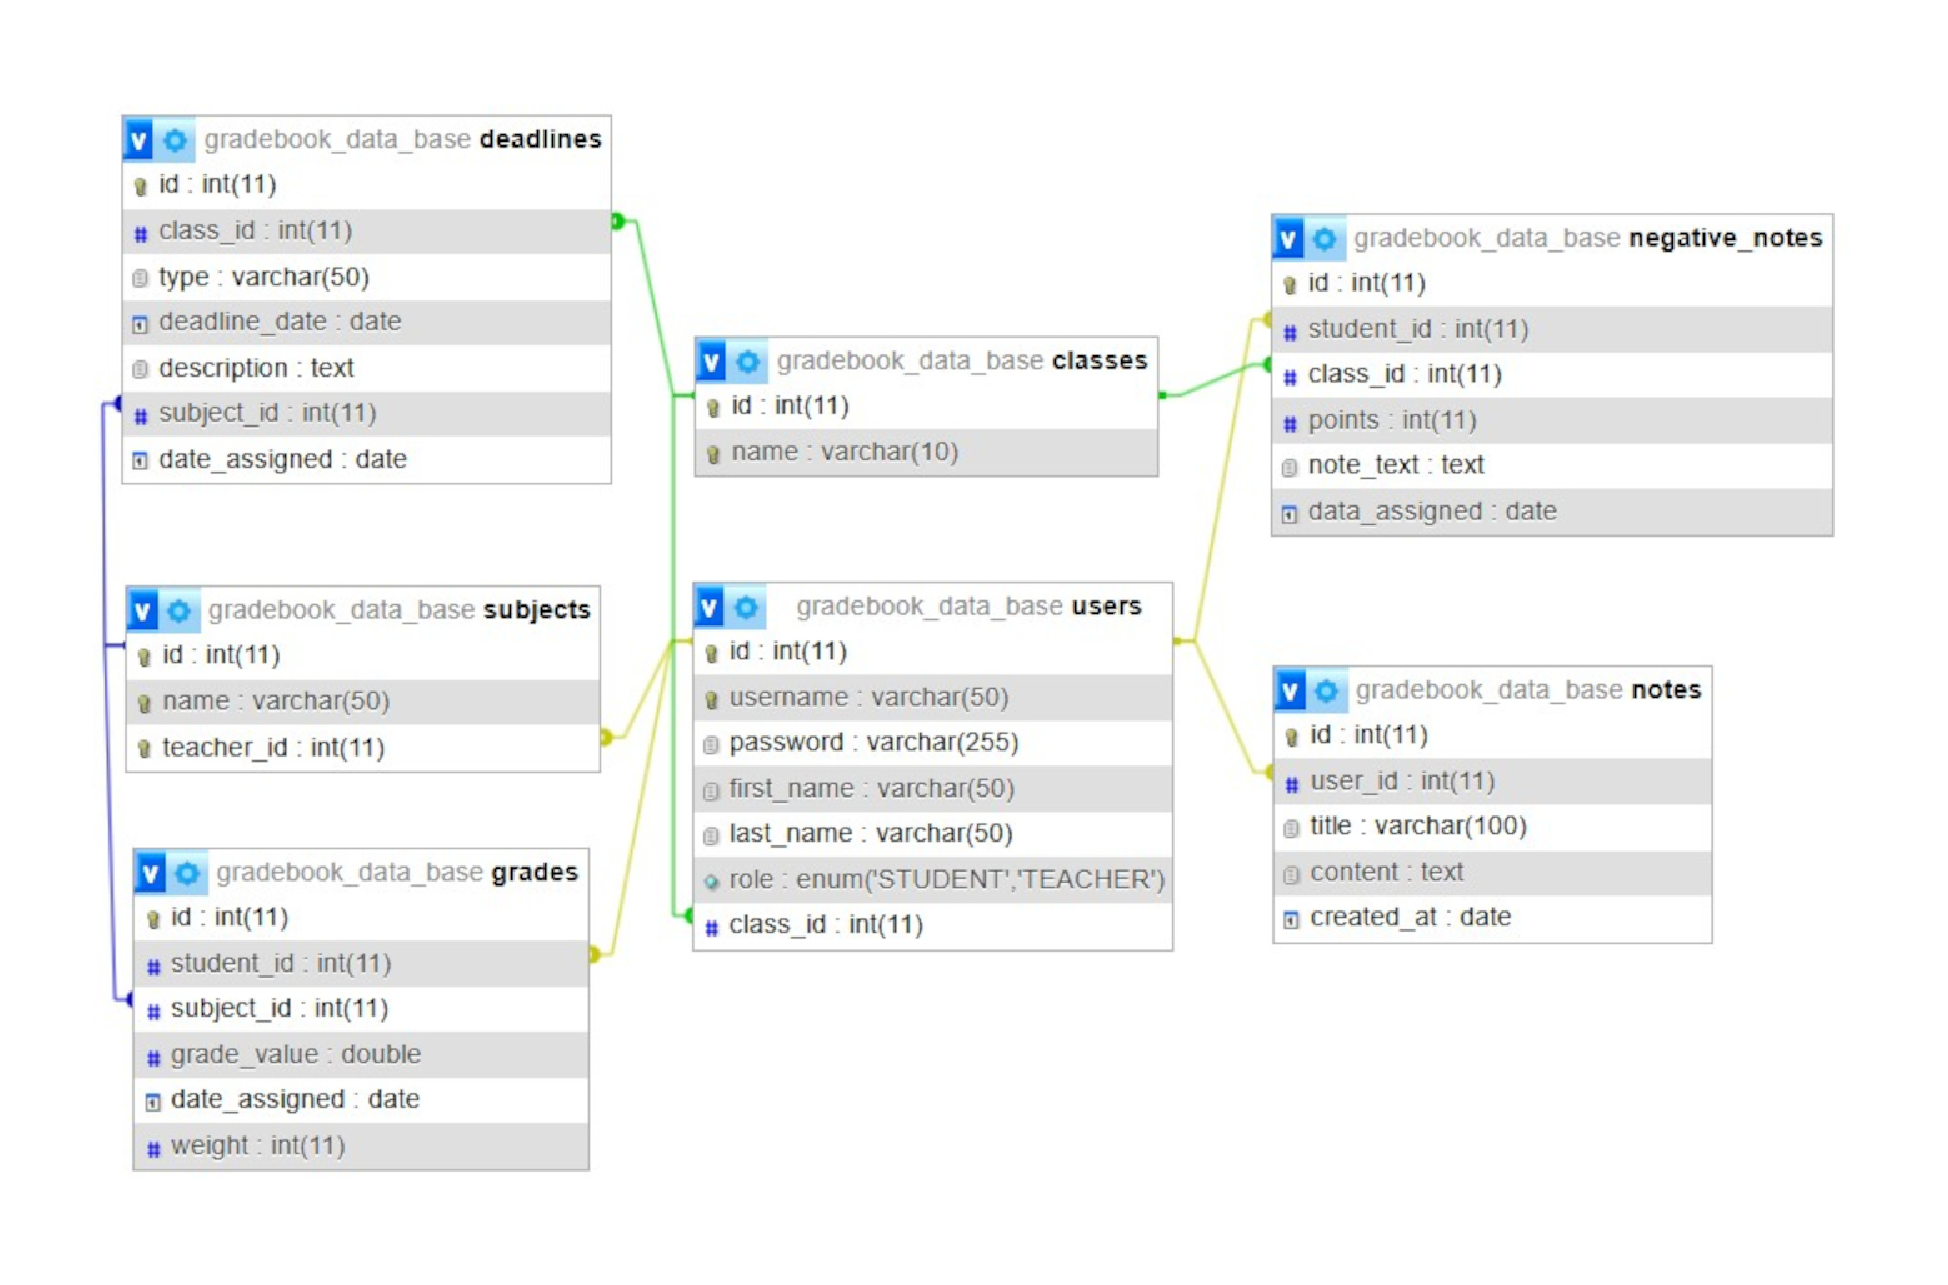
\includegraphics[width=1\textwidth]{figures/fig_0002.eps}
    \caption{Diagram ERD bazy danych \textit{gradebook\_data\_base}}
    \label{fig:erd}
\end{figure}
\newpage
\subsection{Opis tabel}

Struktura bazy danych została zaprojektowana w sposób modularny — każda tabela pełni ściśle określoną funkcję w systemie YLO GradeBook. Tabele powiązane są ze sobą relacjami typu \textit{jeden do wielu} lub \textit{wiele do wielu}, co zapewnia przejrzystość, skalowalność i integralność.

Poniżej przedstawiono opis wszystkich tabel:
\subsubsection*{Tabela \texttt{users}}

Tabela zawiera informacje o wszystkich użytkownikach systemu (uczniach oraz nauczycielach).

\begin{itemize}
    \item \texttt{id} – unikalny identyfikator użytkownika (klucz główny),
    \item \texttt{username}, \texttt{password} – dane logowania,
    \item \texttt{first\_name}, \texttt{last\_name} – dane osobowe,
    \item \texttt{role} – rola użytkownika (np. „student”, „teacher”),
    \item \texttt{class\_id} – odwołanie do tabeli \texttt{classes} (klucz obcy).
\end{itemize}

\subsubsection*{Tabela \texttt{grades}}

Tabela przechowuje oceny przypisywane uczniom.

\begin{itemize}
    \item \texttt{id} – identyfikator oceny (klucz główny),
    \item \texttt{student\_id} – identyfikator ucznia (klucz obcy do \texttt{users}),
    \item \texttt{subject\_id} – przedmiot (klucz obcy do \texttt{subjects}),
    \item \texttt{grade\_value} – wartość oceny (np. 4.5),
    \item \texttt{type} – typ oceny (np. sprawdzian, zadanie),
    \item \texttt{created\_at} – data wystawienia.
\end{itemize}

\subsubsection*{Tabela \texttt{notes}}

Tabela przechowuje notatki osobiste dodawane przez użytkowników systemu.

\begin{itemize}
    \item \texttt{id} – identyfikator notatki (klucz główny),
    \item \texttt{user\_id} – użytkownik, do którego przypisana jest notatka (klucz obcy do \texttt{users}),
    \item \texttt{title} – tytuł notatki,
    \item \texttt{content} – treść notatki,
    \item \texttt{created\_at} – data utworzenia.
\end{itemize}

\subsubsection*{Tabela \texttt{deadlines}}

Tabela przechowuje informacje o nadchodzących terminach.

\begin{itemize}
    \item \texttt{id} – identyfikator terminu (klucz główny),
    \item \texttt{class\_id} – klasa, której dotyczy wydarzenie,
    \item \texttt{subject\_id} – przedmiot związany z terminem,
    \item \texttt{type} – typ wydarzenia (np. sprawdzian, zadanie),
    \item \texttt{date} – data wydarzenia,
    \item \texttt{description} – krótki opis.
\end{itemize}

\subsubsection*{Tabela \texttt{negative\_notes}}

Tabela służy do zapisywania uwag pozytywnych i negatywnych przypisanych uczniom.

\begin{itemize}
    \item \texttt{id} – identyfikator uwagi (klucz główny),
    \item \texttt{student\_id} – uczeń, którego dotyczy uwaga,
    \item \texttt{class\_id} – klasa ucznia,
    \item \texttt{points} – liczba punktów (ujemne/dodatnie),
    \item \texttt{message} – treść uwagi (do 60 znaków),
    \item \texttt{created\_at} – data wystawienia.
\end{itemize}

\subsubsection*{Tabela \texttt{subjects}}

Tabela zawiera przedmioty występujące w systemie.

\begin{itemize}
    \item \texttt{id} – identyfikator przedmiotu (klucz główny),
    \item \texttt{name} – nazwa przedmiotu (np. „matematyka”),
    \item \texttt{teacher\_id} – nauczyciel prowadzący (klucz obcy do \texttt{users}).
\end{itemize}

\subsubsection*{Tabela \texttt{classes}}

Lista klas funkcjonujących w systemie.

\begin{itemize}
    \item \texttt{id} – identyfikator klasy (klucz główny),
    \item \texttt{name} – nazwa klasy (np. „1TIA”),
    \item \texttt{school\_year} – rok szkolny przypisany do klasy.
\end{itemize}


\subsection{Relacje między tabelami}

Relacje pomiędzy tabelami w bazie \textit{gradebook\_data\_base} zostały zaprojektowane w sposób zapewniający pełną integralność danych oraz umożliwiający logiczne powiązanie informacji pomiędzy różnymi obiektami systemu.

\begin{itemize}
     \item Każdy użytkownik (\texttt{users}) przypisany jest do konkretnej klasy (\texttt{classes}), co pozwala na filtrowanie danych względem przynależności uczniów. 
     \item Użytkownicy mogą pełnić rolę ucznia lub nauczyciela, dzięki czemu możliwe jest rozdzielienie funkcjonalność dla obu grup. 
     \item Oceny (\texttt{grades}) są powiązane zarówno z użytkownikiem (uczniem), jak i przedmiotem (\texttt{subjects}), którego dotyczą.      \item Terminy (\texttt{deadlines}) są przypisane do konkretnej klasy i odnoszą się do określonego przedmiotu. \item Notatki (\texttt{notes}) tworzone są indywidualnie przez użytkowników i przypisane tylko do ich kont. 
     \item Uwagi (\texttt{negative\_notes}) są przypisane do ucznia oraz zawierają liczbę punktów (ujemnych lub dodatnich) i treść. 
\end{itemize}

\section*{Podsumowanie}

Struktura bazy danych \textit{gradebook\_data\_base} została zaprojektowana z myślą o przejrzystości, integralności oraz skalowalności danych. Dzięki odpowiednio powiązanym encjom, system pozwala na jednoznaczną identyfikację użytkowników, przypisywanie ocen, notatek, terminów i uwag w kontekście klas i przedmiotów. Zaprojektowana architektura relacyjna nie tylko wspiera bieżącą funkcjonalność aplikacji, ale umożliwia także łatwą rozbudowę systemu w przyszłości — zarówno pod względem danych, jak i logiki aplikacyjnej.

\newpage\newpage
\section{Struktura aplikacji}
\label{sec:strukturaAplikacji}

Aplikacja \textit{YLO GradeBook} została stworzona w języku \textbf{Java} z wykorzystaniem biblioteki \textbf{JavaFX}. Struktura projektu podzielona została na warstwy odpowiadające za logikę, prezentację danych, komunikację z bazą danych oraz wartswę wizualną.

\subsection{Struktura pakietów w projekcie}

Aplikacja \texttt{YLO GradeBook} posiada podział na kilka głównych części: 

\begin{itemize}
    \item \texttt{pakiet główny} – zawiera wszystkie klasy aplikacji odpowiedzialne za:
    \begin{itemize}
        \item logikę kontrolerów powiązanych z plikami \texttt{.fxml},
        \item klasę startową \texttt{Main.java},
        \item połączenie z bazą danych (\texttt{DataBaseConnection.java}),
        \item klasy pomocnicze
    \end{itemize}

    \item \texttt{models} – pakiet zawierający klasy odwzorowujące encje z bazy danych. Każdy model reprezentuje jedną tabelę.
    \item \texttt{resources} – pakiet zawierający pliki wykorzystywane w warstwie prezentacji, takie jak:
    \begin{itemize}
        \item pliki FXML opisujące strukturę widoków graficznych,
        \item style CSS odpowiadające za wygląd interfejsu,
        \item czcionki i ikony wykorzystywane w interfejsie użytkownika.
    \end{itemize}
\end{itemize}

Chociaż klasy w pakiecie głównym nie zostały podzielone na pod-pakiety ze względu na funkcjonalność, zastosowano odpowiednie nazewnictwo, które jasno określa ich przeznaczenie. Dzięki temu struktura pozostaje spójna i zrozumiała.

\subsection{Opis zaimplementowanych klas}

Diagram klas (rys. \ref{fig:diagramUML}) przedstawia strukturę głównych komponentów systemu, ich wzajemne relacje dziedziczenia oraz implementację. 
\subsubsection*{Main.java}
Klasa startowa aplikacji. Zawiera metodę \texttt{start()} z JavaFX i ładuje widok logowania (\texttt{LoginWindow.fxml}). Odpowiada za inicjalizację sceny głównej i ustawienie tytułu aplikacji.

\subsubsection*{DataBaseConnection.java}
Klasa służy do połączenia z bazą danych \texttt{MySQL}. Wykorzystuje sterownik JDBC oraz dane logowania zapisane w kodzie.

\subsubsection*{MainWindow.java}
Klasa pełniąca zadanie kontrolera dla głównego kontenera (\texttt{MainWindow.fxml}) do ładowania poszczególnych widoków.

\subsubsection*{ViewLoadingManager.java}
Klasa pomocnicza pełniąca funkcję menadżera ładowania widoków. Każda metoda przyjmuje nazwę pliku \texttt{.fxml} i zastępuje bieżący widok w kontenerze \texttt{MainWindow.fxml}.

\subsubsection*{Session.java}
Klasa pomocnicza przechowująca informacje o zalogowanym użytkowniku, dzięki czemu w trakcie trwania sesji aplikacji mamy dostęp do jego danych.

\subsubsection*{SessionController.java}
Abstrakcyjna klasa bazowa zawierająca metody do wyświetlania komunikatów systemowych (błędy, ostrzeżenia, informacje). Umożliwia klasom pochodnym stosowanie jednolitego mechanizmu komunikacji z użytkownikiem, eliminując powielanie kodu.

\subsubsection*{AuthenticationInterface.java}
W strutkturze skorzystano z możliwości implementacji interfejsu, który wymusza na klasach go implementujących zdefiniowanie odpowiednich metod. Metody, które implementuje umożliwiają pokazywanie hasła podczas logowania lub resetowania hasła oraz pozwalające na włączenie możliwości przemieszczanie się tabulatorem po interfejsie użytkownika.

\subsubsection*{LoginWindow.java}
Kontroler powiązany z widokiem \texttt{LoginWindow.fxml}. Odpowiada za logowanie użytkownika i zapis jego danych w klasie \texttt{Session}. Implementuje interfejs \texttt{AuthenticationInterface}, co umożliwia m.in. obsługę pokazywania hasła oraz przełączanie fokusu tabulatorem. Udostępnia również metodę otwierającą widok resetowania hasła.

\subsubsection*{PasswordReset.java}
Kontroler przypisany do widoku \texttt{PasswordReset.fxml}. Pozwala na aktualizację hasła użytkownika po podaniu poprawnych danych. Również implementuje interfejs \texttt{AuthenticationInterface} i definiuje odpowiednie metody zgodne z tym widokiem.

\subsubsection*{StudentWindow.java}
Kontroler odpowiadający za widok \texttt{StudentWindow.fxml}. Odpowiada za obsługę graficznego interfejsu ucznia, który zawiera panele z ocenami, terminami, uwagami oraz notatkami osobistymi. Klasa odpowiada m.in. za:
\begin{itemize}
    \item ładowanie i aktualizowanie danych ucznia (oceny, średnia, uwagi, terminy),
    \item filtrowanie wpisów dodanych w ciągu ostatnich 7 dni,
    \item obsługę notatek użytkownika (dodawanie i usuwanie),
    \item przełączanie widoków i obsługę przycisków w panelu bocznym,
    \item dostęp do widoków danych osobowych oraz zmiany hasła.
\end{itemize}
\newpage
\subsubsection*{TeacherWindow.java}
Kontroler widoku \texttt{TeacherWindow.fxml}, pełniący funkcję głównego panelu nauczyciela. Klasa umożliwia:
\begin{itemize}
    \item przegląd uczniów przypisanych do wybranej klasy,
    \item przegląd i analizę ocen z podziałem na przedmioty i uczniów,
    \item dodawanie ocen, terminów, uwag oraz notatek osobistych,
    \item zarządzanie widokiem danych osobowych i zmiany hasła,
    \item przełączanie sekcji aplikacji za pomocą panelu nawigacyjnego.
\end{itemize}

\subsubsection*{PopUpWindow.java}
Klasa pomocnicza obsługująca otwieranie widoków typu \textit{popup} w osobnych oknach. Umożliwia ładowanie plików \texttt{.fxml} zawierających formularze, np. do dodawania ocen, terminów, notatek czy uwag. Zapewnia spójny i modularny sposób wyświetlania dodatkowych interfejsów użytkownika bez zakłócania głównego widoku.

\subsection{Modele}
\label{sec:moduly}

W strukturze systemu zastosowano modele odpowiadające tabelom bazy danych, co umożliwia odwzorowanie danych w postaci obiektów Java. Każda klasa modelowa zawiera zestaw atrybutów reprezentujących kolumny w tabeli oraz odpowiednie metody dostępowe (gettery i settery).

\begin{itemize}
    \item \texttt{Classes.java} – reprezentuje klasę uczniowską; zawiera m.in. nazwę klasy.
    \item \texttt{Deadlines.java} – odwzorowuje terminy wydarzeń przypisanych do klas i przedmiotów, takich jak sprawdziany czy kartkówki.
    \item \texttt{Grade.java} – odpowiada za pojedynczą ocenę ucznia.
    \item \texttt{NegativeNote.java} – przechowuje informacje o punktowych uwagach przypisanych do uczniów, zarówno pozytywnych, jak i negatywnych.
    \item \texttt{Note.java} – model notatki utworzonej przez użytkownika, zawierający tytuł i treść.
    \item \texttt{StudentGrade.java} – pomocniczy model wykorzystywany do wyświetlania ocen z przypisanym przedmiotem i obliczoną średnią ocen.
    \item \texttt{Subject.java} – reprezentuje przedmiot szkolny.
    \item \texttt{Users.java} – ogólny model użytkownika systemu (ucznia lub nauczyciela), przechowujący dane logowania, imię, nazwisko i rolę.
\end{itemize}

\section*{}
\begin{figure}[H]
    \centering
    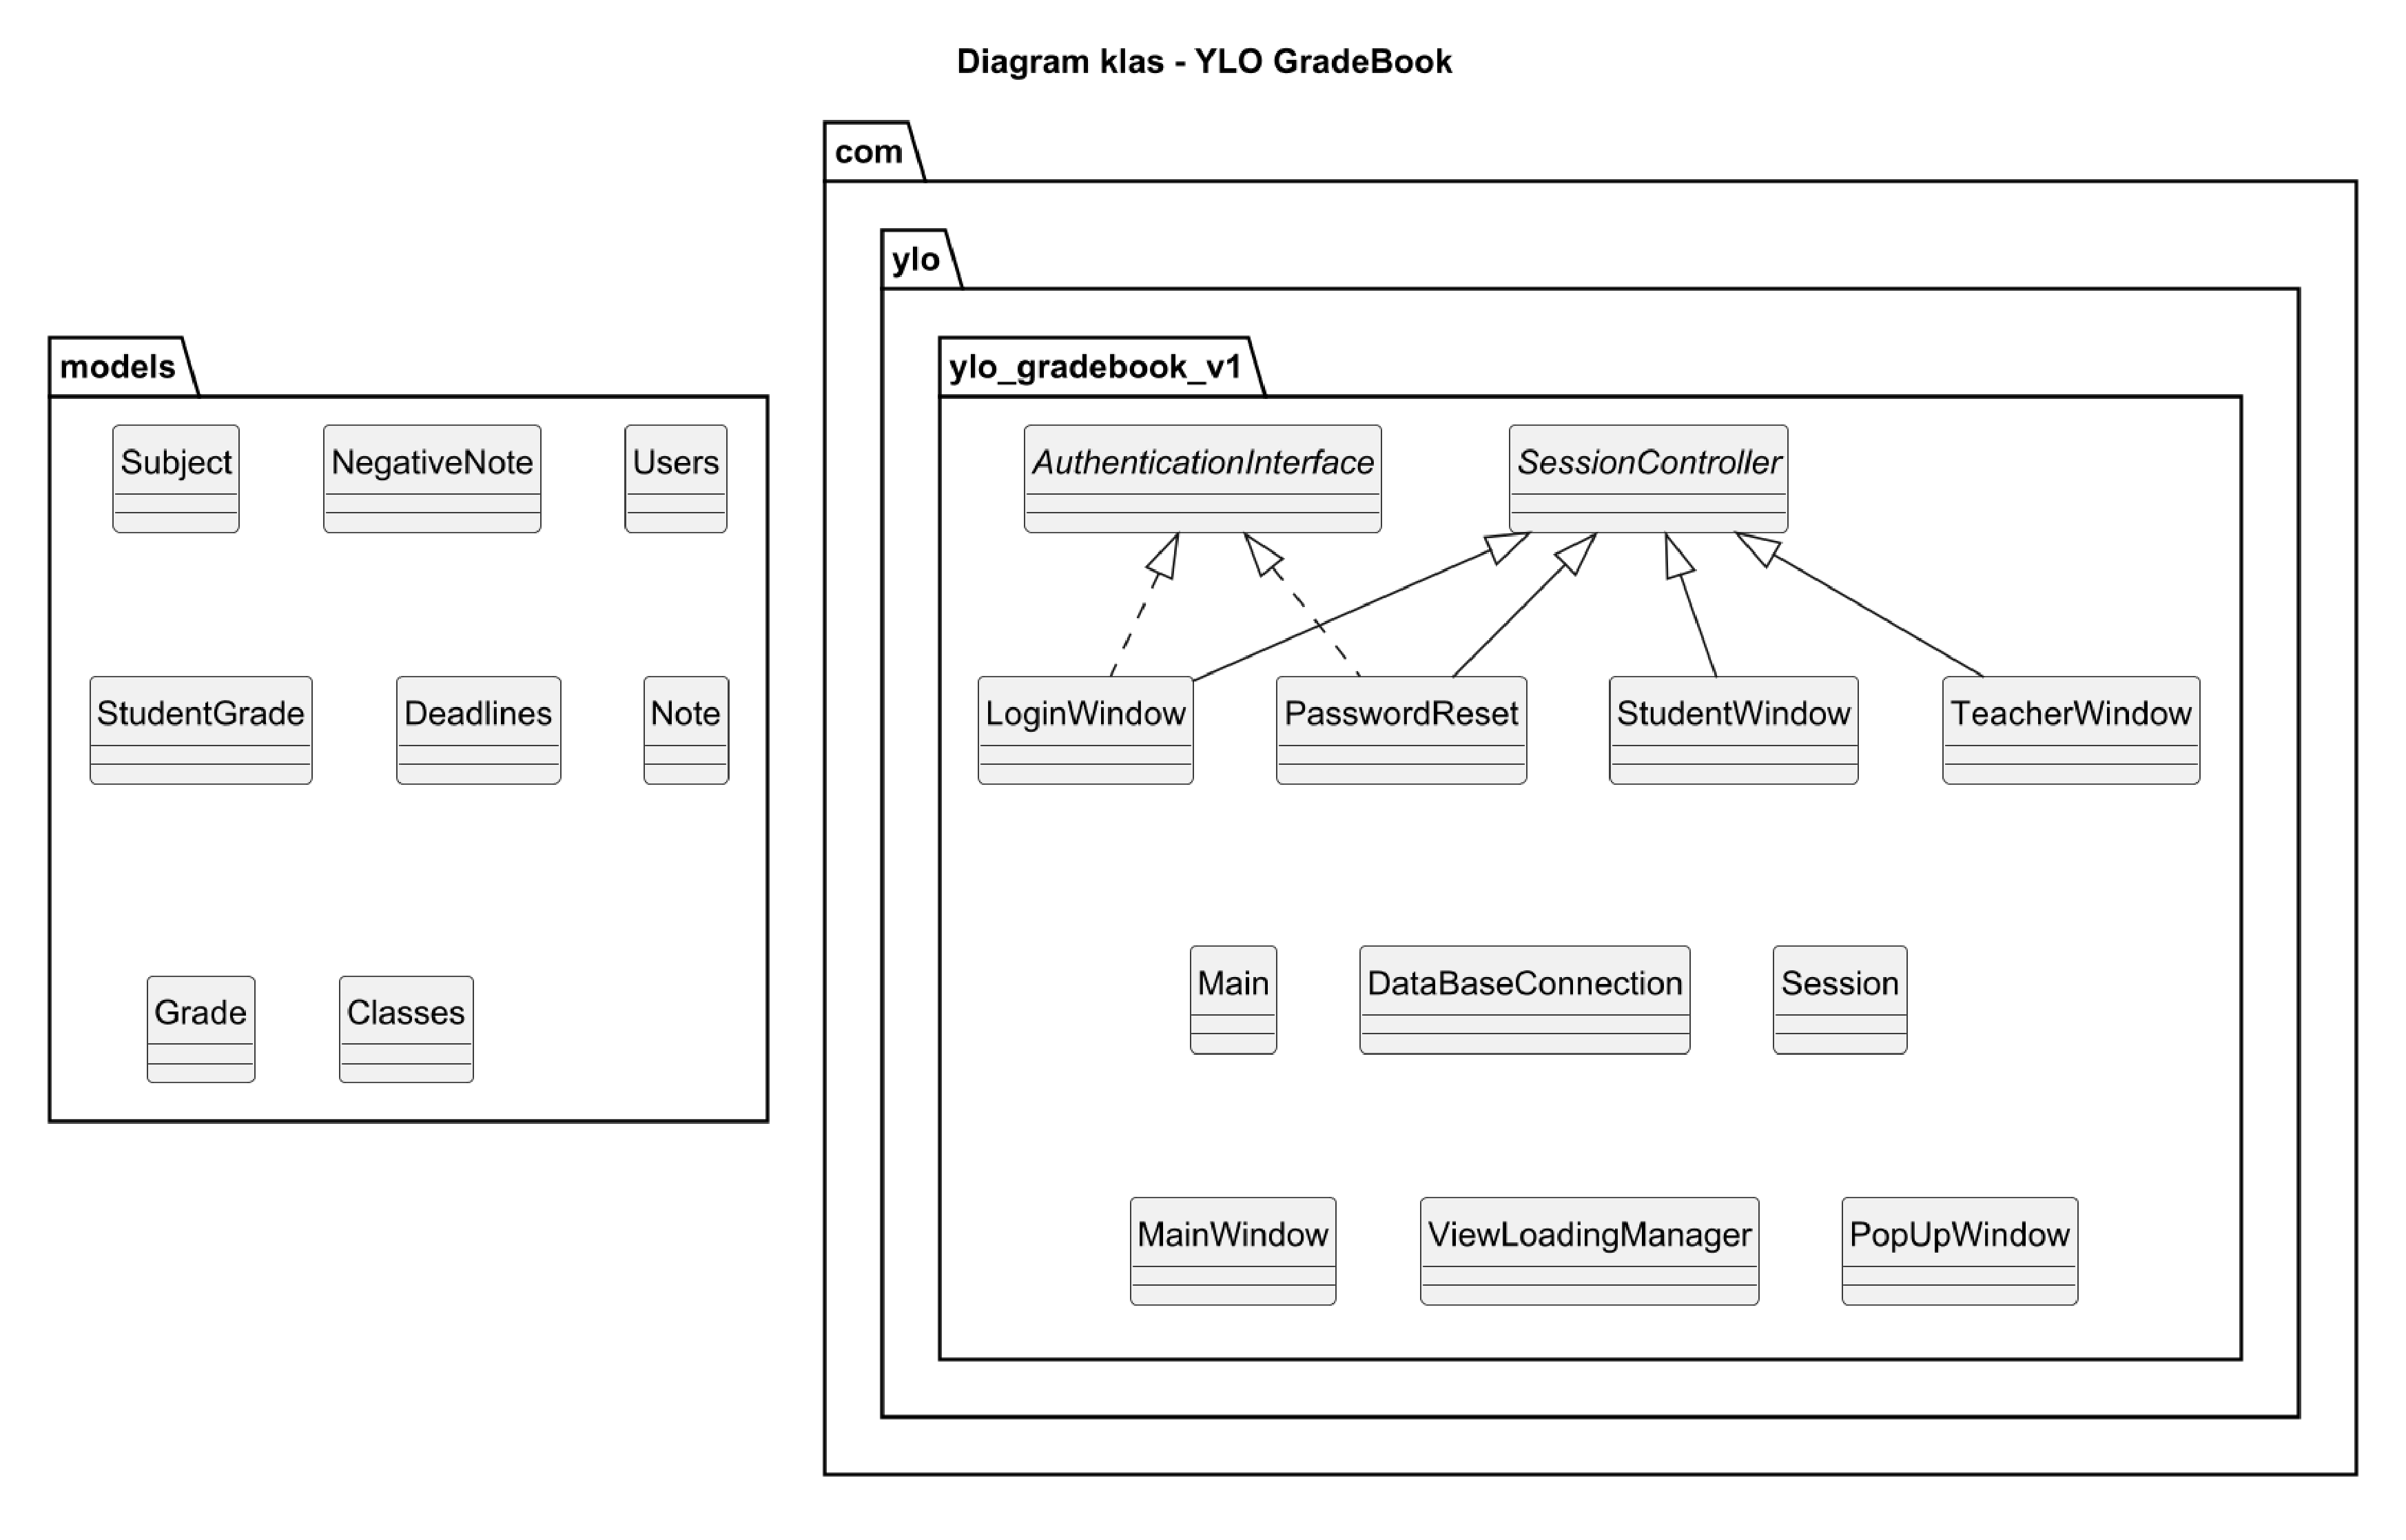
\includegraphics[width=1\textwidth]{figures/fig_0003.eps}
    \caption{Diagram klas systemu YLO GradeBook}
    \label{fig:diagramUML}
\end{figure}



\subsection{Widoki graficzne (FXML)}
\label{sec:widokiFXML}

Interfejs użytkownika aplikacji \texttt{YLO GradeBook} został zaprojektowany z użyciem technologii \textbf{FXML}, co umożliwia oddzielenie warstwy wizualnej od logiki aplikacji. Każdy plik FXML odpowiada konkretnemu widokowi i powiązany jest ze swoim kontrolerem w języku \texttt{Java}.

\begin{itemize}
    \item \texttt{MainWindow.fxml} – główny kontener aplikacji, do którego ładowane są pozostałe widoki (ucznia lub nauczyciela). Stanowi miejsce dynamicznie zmieniających się widoków.
    \item \texttt{LoginWindow.fxml} – widok logowania. Zawiera pola do wpisania loginu i hasła, przycisk logowania oraz odnośnik do resetowania hasła. Umożliwia użytkownikowi dostęp do systemu.
    \item \texttt{PasswordReset.fxml} – formularz zmiany hasła. Zawiera pola do wprowadzenia loginu, nowego hasła i jego potwierdzenia.
    \item \texttt{PopUpWindow.fxml} – szablon wykorzystywany do wyświetlania popupów, np. do dodawania ocen, terminów, notatek czy uwag. Umożliwia ładowanie okien pomocniczych bez zakłócania pracy głównej aplikacji.
    \item \texttt{StudentWindow.fxml} – główny widok ucznia. Zawiera pasek nawigacyjny, umożliwiający przełączanie się pomiędzy wieloma zakładkami. Zawiera rozbudowaną strukturę, która realizuje wszystkie funkcje udostępnione dla roli ucznia.
    \item \texttt{TeacherWindow.fxml} – główny widok nauczyciela. Udostępnia pełną funkcjonalność do zarządzania danymi. Podobnie jak widok ucznia posiada panel nawigacyjny do przełączania się między zakładkami.
\end{itemize}

\subsection{Pozostałe zasoby}
Folder \texttt{resources} zawiera nie tylko pliki FXML odpowiadające widokom graficznym, ale także zasoby wizualne, które wspierają spójny i nowoczesny wygląd aplikacji. W jego strukturze znajdują się:
\begin{itemize}
    \item \texttt{styles/} – pliki CSS definiujące styl graficzny aplikacji. Wpływają one na kolory, marginesy, zaokrąglenia przycisków i ogólną estetykę interfejsu użytkownika.
    \item \texttt{icons/} – zestaw ikon w formacie \texttt{.png}, wykorzystywany w przyciskach, paskach nawigacyjnych i oknach popup. Ułatwiają szybką identyfikację funkcji.
    \item \texttt{fonts/} – pliki czcionek używane w interfejsie. Ich dołączenie zapewnia spójność typograficzną.
\end{itemize}

Zestaw ikon użytych w interfejsie graficznym pochodzi ze strony \texttt{www.freepik.com}. Ikony zostały pobrane w ramach licencji wymagającej przypisania autorstwa i były modyfikowane graficznie na potrzeby projektu.  

Zastosowanie zasobów oddzielonych od logiki aplikacji zwiększa przejrzystość projektu i ułatwia jego stylowanie bez ingerencji w kod źródłowy.

\chapter{Harmonogram realizacji projektu}
\label{cha:harmonogram}

\section{Etapy realizacji oraz wykres Gantta}

Proces tworzenia aplikacji \texttt{YLO GradeBook} został zaplanowany jako ciąg kolejnych etapów, obejmujących m.in. analizę wymagań, projektowanie architektury, tworzenie interfejsu użytkownika, implementację logiki systemu, testowanie oraz przygotowanie dokumentacji technicznej.

Realizacja przebiegała zgodnie z przyjętym harmonogramem, jednak w trakcie realizacji konieczne było kilkukrotne cofnięcie się do wcześniejszych faz projektu — w celu wprowadzenia poprawek lub dostosowania struktury do nowych funkcjonalności.

Warto podkreślić, że wiele zadań prowadzono równolegle, ponieważ dawało to swobodę realizacji nowych pomysłów. 

W celu zobrazowania kolejnych faz projektu, opracowano wykres Gantta (rys. \ref{fig:ganttYLO}) przedstawiający plan pracy.


\begin{figure}[H]
    \centering
    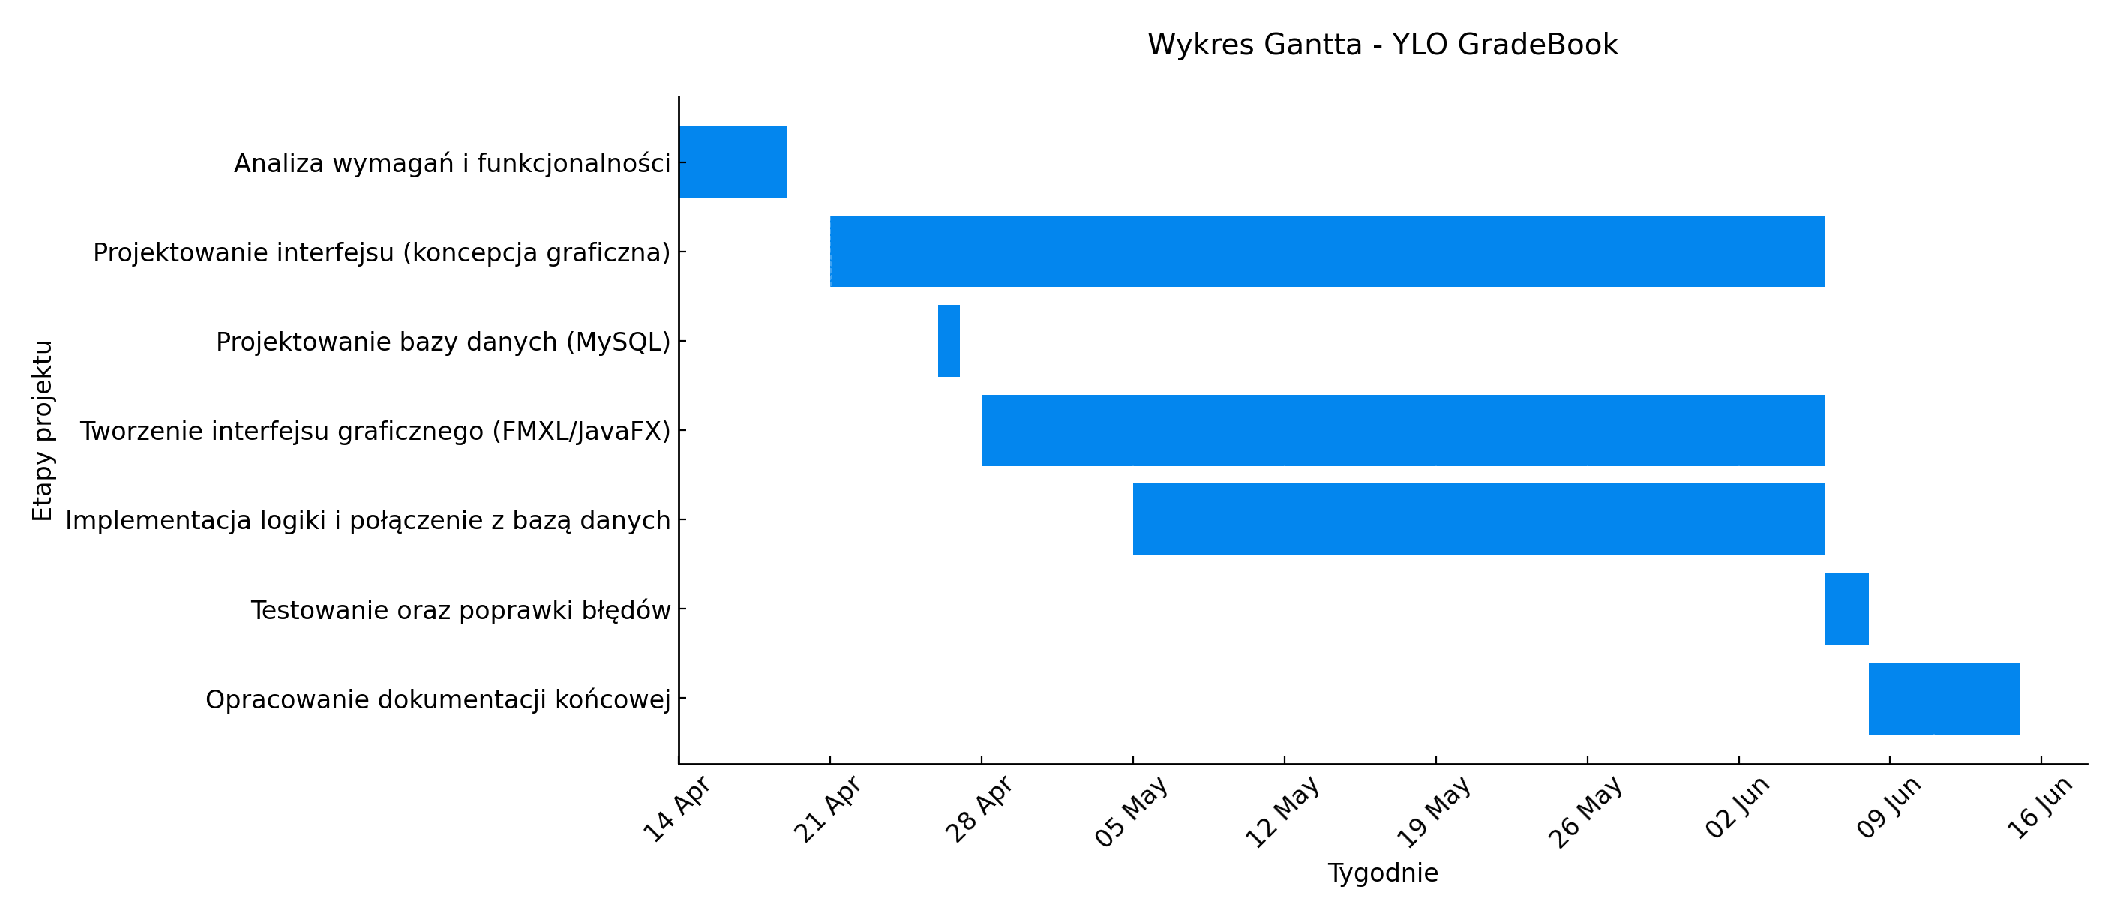
\includegraphics[width=1\textwidth]{figures/fig_0004.eps}
    \caption{Wykres Gantta przedstawiający harmonogram realizacji projektu YLO GradeBook}
    \label{fig:ganttYLO}
\end{figure}

\section{System kontroli wersji i repozytorium projektu}

W trakcie realizacji projektu wykorzystano system kontroli wersji \textbf{Git}, który umożliwił systematyczne zapisywanie kodu.  Do przechowywania i synchronizacji kodu źródłowego użyto platformy \textbf{GitHub}.

Pełne repozytorium projektu \texttt{YLO GradeBook} jest dostępne pod adresem:

\begin{center}
\texttt{https://github.com/oleiy/YLO-GradeBook}
\end{center}

Repozytorium zawiera ostateczną wersję projektu, okumentację projektowa oraz bazę danych. Zgodnie z wymaganiami, projekt dostępny będzie przez cały rok.
\chapter{Prezentacja warstwy użytkowej projektu}
\label{cha:prezentacja}


Warstwa użytkowa aplikacji \texttt{YLO GradeBook} została opracowana z myślą o intuicyjności, estetyce oraz ergonomii użytkowania. Interfejs powstał przy użyciu technologii \textbf{JavaFX}, a do jego definiowania wykorzystano pliki \textbf{FXML}, co umożliwiło czytelne oddzielenie logiki od prezentacji. W projekcie zastosowano również kaskadowe arkusze stylów CSS w celu zdefiniowania wyglądu widoków.

W tym rozdziale zaprezentowano strukturę graficzną głównych widoków aplikacji wraz z opisem funkcji dostępnych dla poszczególnych ról użytkownika (uczeń/nauczyciel). Dodatkowo omówiono styl graficzny interfejsu (kolorystyka, czcionki, ikony) oraz zastosowane mechanizmy wspomagające interakcję z systemem (komunikaty, formularze, walidacja danych).

\section{Opis szaty graficznej interfejsu}
Zastosowana kolorystyka interfejsu opiera się na stonowanej palecie odcieni niebieskiego, bieli i jasnej szarości, co sprzyja przejrzystości i komfortowi wizualnemu użytkownika. Dominujące barwy zostały dobrane w taki sposób, aby nie rozpraszać, a jednocześnie nadawać aplikacji nowoczesny i estetyczny wygląd.

\begin{itemize}
    \item \textbf{rgb(3,134,238)} — intensywny niebieski wykorzystywany do przycisków.
    \item \textbf{rgb(220,220,220)} — jasnoszare tło głównego widoku, stanowiące neutralne tło dla treści,
    \item \textbf{rgb(255,255,255)} oraz \textbf{rgb(245,245,245)} — używane dla zwiększenia czytelności sekcji,
    \item \textbf{rgb(238,248,255)} — wyróżnienie niektórych elementów np. główny przycisk w sekcji.
    \item \textbf{rgb(220,220,220)} — kolor ramek róznych elementów interfejsu.
\end{itemize}

Taka paleta kolorów nie tylko spełnia funkcje estetyczne, ale również wpływa na ergonomię oraz odczucia użytkownika w trakcie korzystania z aplikacji.

Dodatkowym elementem nadającym interfejsowi nowoczesny charakter jest zastosowanie czcionki \textbf{Poppins} — geometrycznego, bezszeryfowego kroju pisma, który zapewnia doskonałą czytelność i estetykę. 

Ponadto w całej aplikacji wykorzystano delikatne zaokrąglenia rogów przycisków, kart i paneli, co — w połączeniu z jasną kolorystyką i minimalistycznym układem — nadaje całości subtelnie \textit{futurystyczny wygląd}, przy jednoczesnym zachowaniu prostoty oraz przejrzystości układu graficznego.

\section{Prezentacja głównych widoków interfejsu użytkownika}

W tej sekcji przedstawiono główne widoki interfejsu użytkownika aplikacji \texttt{YLO GradeBook} wraz z opisem ich funkcjonalności i przeznaczenia. Każdemu ekranowi towarzyszy zrzut ekranu ukazujący jego wygląd oraz interakcje z użytkownikiem.

Przedstawione zrzuty ekranu pochodzą z sesji użytkowników: ucznia o nazwie \texttt{Igor Lis} oraz nauczyciela \texttt{Jan Nowak}. Wykorzystano je w celu zaprezentowania widoków odpowiadających poszczególnym rolom w systemie.

\subsection{Okno logowania}
Widok logowania stanowi punkt wejścia do aplikacji i umożliwia użytkownikowi dostęp do systemu poprzez weryfikację jego danych uwierzytelniających.
\begin{itemize}
    \item Interfejs zawiera dwa pola wejściowe: \textbf{Nazwa użytkownika} oraz \textbf{Hasło}, przycisk \textbf{Zaloguj się}, a także opcję \textbf{Nie pamiętasz hasła?}, umożliwiająca resetowanie hasła.
    \item Posiada również możliwość pokazania hasła, za pomocą intuicyjnego przycisku na polu hasła.
    \item W przypadku błędnego logowania pojawia się odpowiedni komunikat walidacyjny.
\end{itemize}

\begin{figure}[H]
    \centering
    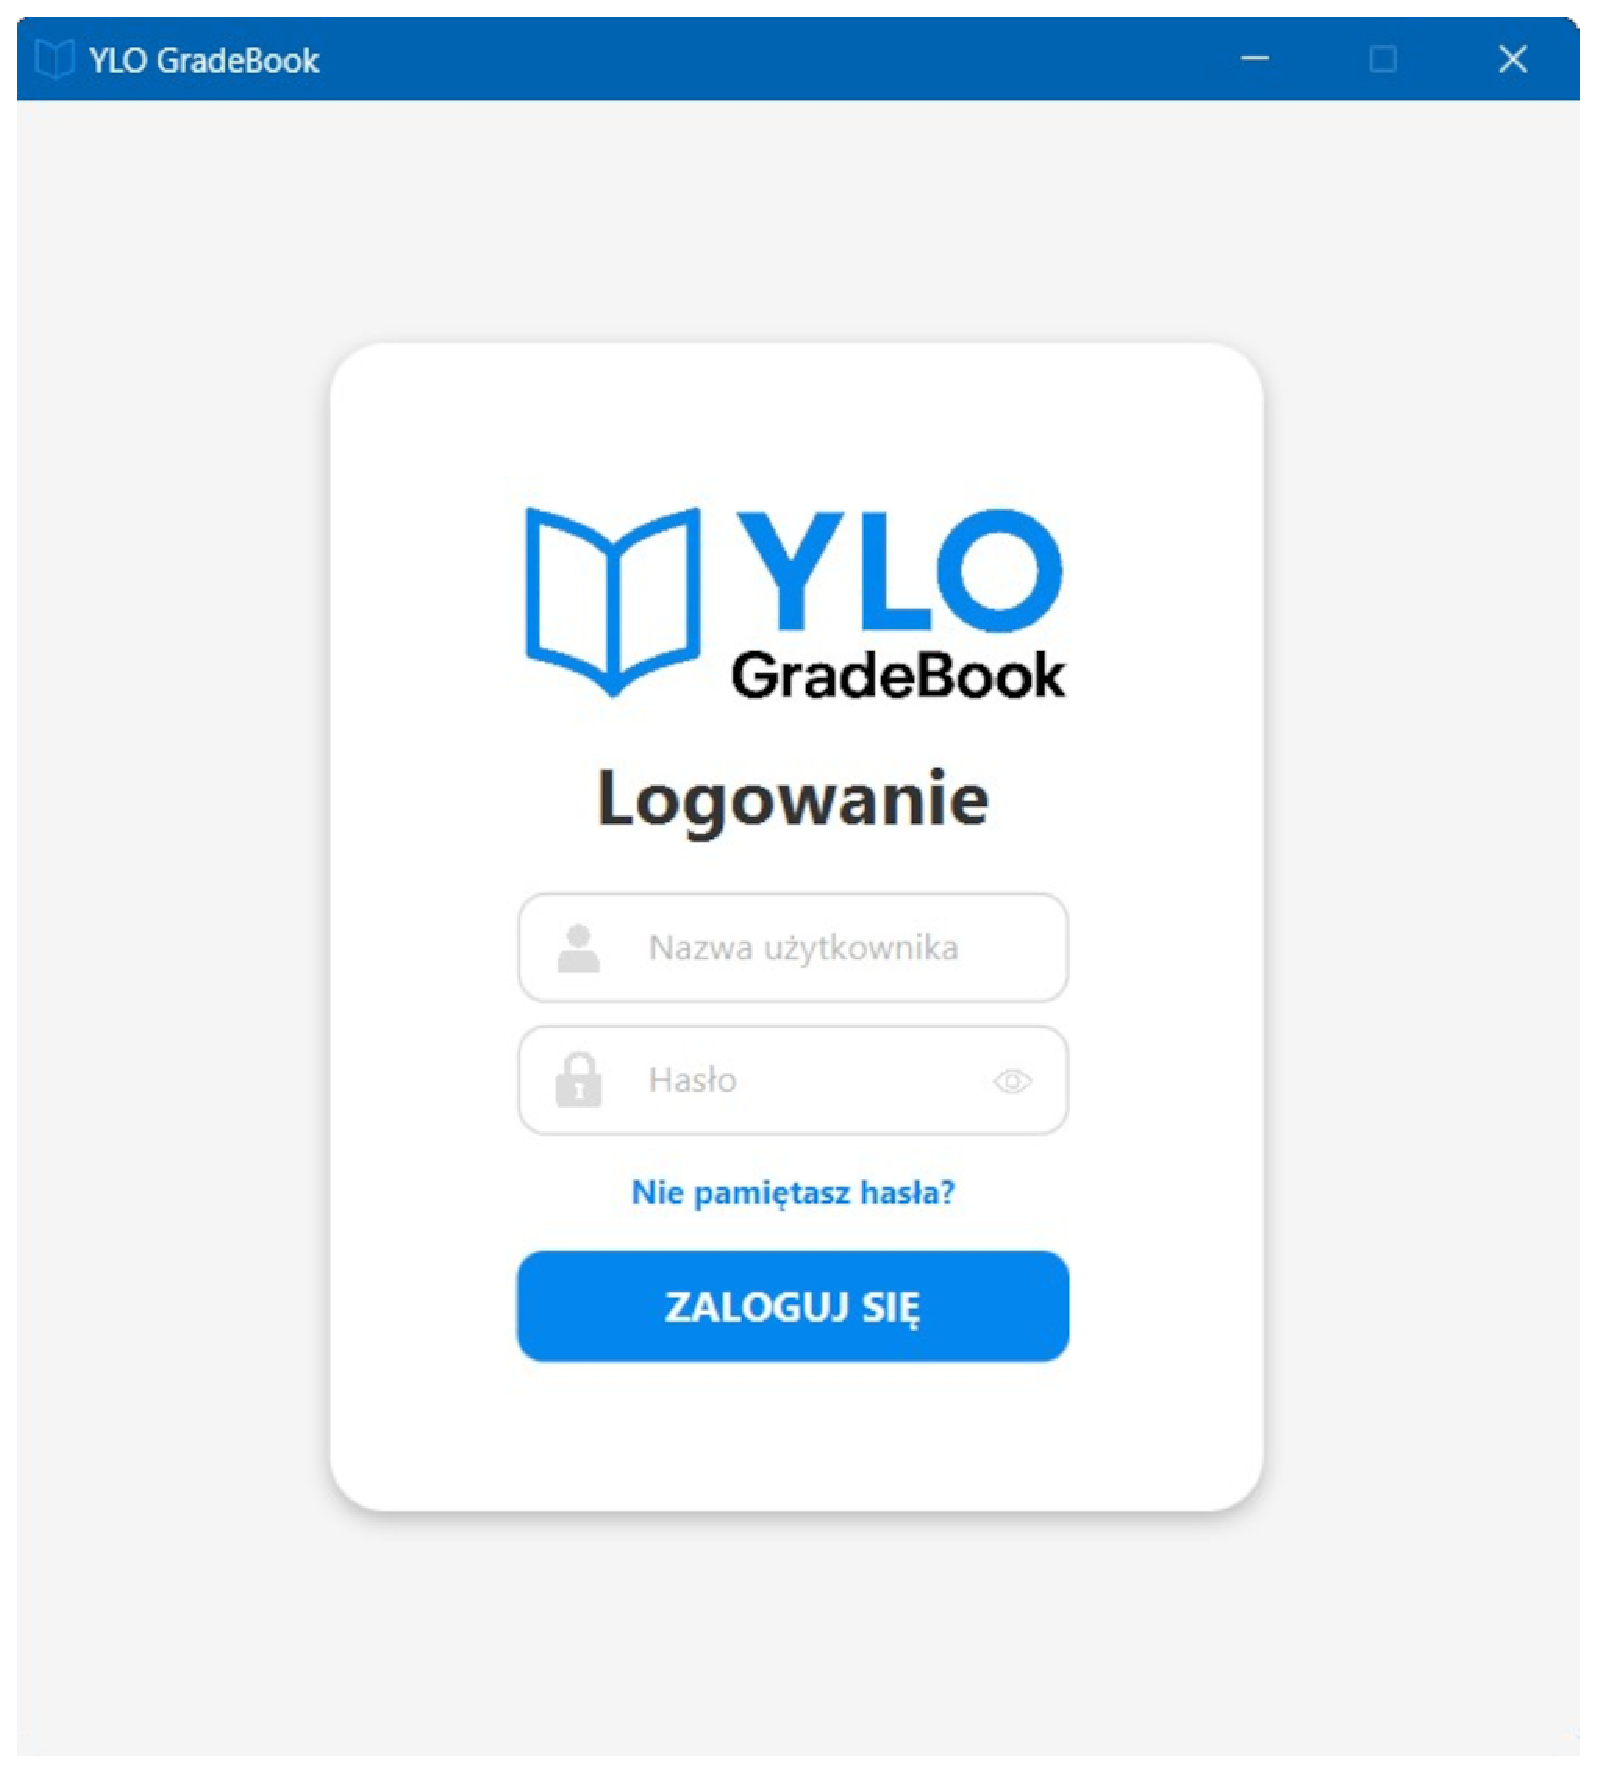
\includegraphics[width=0.9\textwidth]{figures/fig_0005.eps}
    \caption{Okno logowania - weryfikacja danych uwierzytelniających}
    \label{fig:loginView}
\end{figure}
\newpage
\subsection{Okno resetowania hasła}
Widok ten umożliwia zresetowanie hasła użytkownika poprzez podanie jego nazwy konta oraz nowego hasła. Na tym etapie proces nie zawiera jeszcze pełnych mechanizmów bezpieczeństwa (np. weryfikacji mailowej), jednak przewidziano ich wdrożenie w przyszłych wersjach aplikacji.

\begin{itemize}
    \item Interfejs posiada trzy pola: \textbf{Nazwa użytkownika}, \textbf{Hasło} oraz \textbf{Potwierdź hasło}. Posiada również przycisk \textbf{Anuluj} oraz przycisk \textbf{Resetuj hasło}, który pozwala na zaaktualizowanie hasła w bazie danych.
    \item Podobnie jak w przypadku okna logowania dodano możliwość wyświetlenia haseł.
    \item W przypadku błędnego wypełnienia pól pojawia się komunikat.
\end{itemize}

\begin{figure}[H]
    \centering
    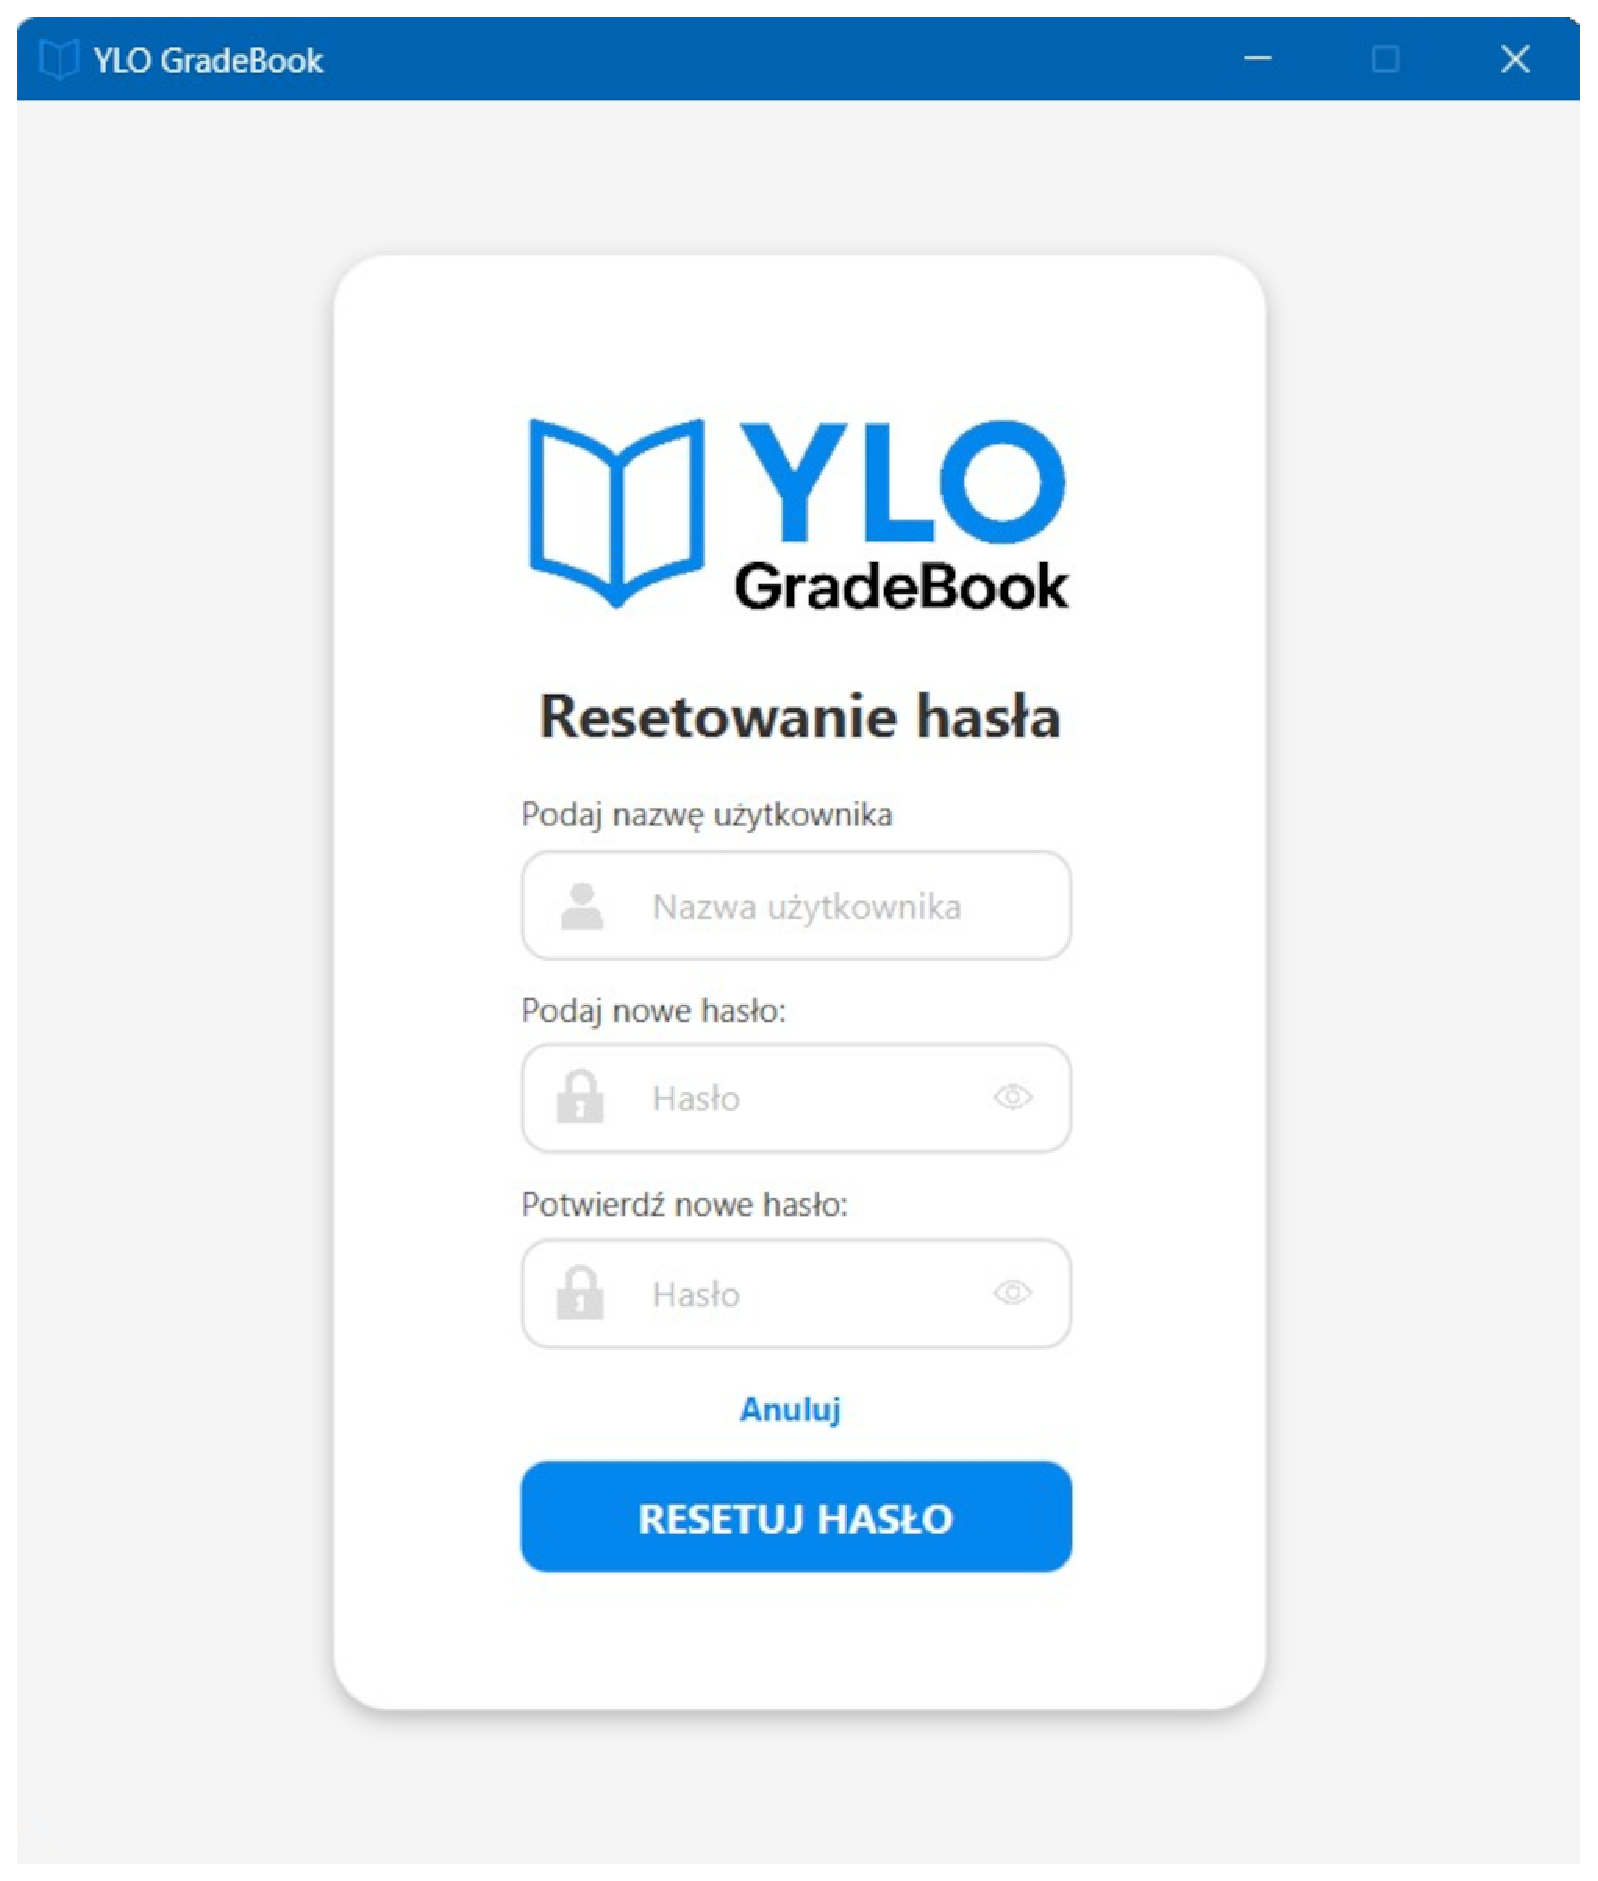
\includegraphics[width=0.9\textwidth]{figures/fig_0006.eps}
    \caption{Okno resetowania hasła - aktualizacja hasła w bazie danych}
    \label{fig:passwordReset}
\end{figure}


\subsection{Główne okno interfejsu ucznia}

Główne okno interfejsu ucznia pojawia się bezpośrednio po jego zalogowaniu do systemu \texttt{YLO GradeBook}. Zostało zaprojektowane z myślą o szybkim i intuicyjnym dostępie do najważniejszych informacji oraz funkcji systemu. Podział treści na zakładki oraz wyraźna struktura ułatwiają poruszanie się po aplikacji.

\begin{itemize}
    \item Po lewej stronie znajduje się panel nawigacyjny z zakładkami: \textbf{Strona główna}, \textbf{Oceny}, \textbf{Terminarz}, \textbf{Uwagi}, \textbf{Notatki}, \textbf{Konto} oraz \textbf{Ustawienia}.
    \item W górnej części widoku wyświetlane jest powitanie użytkownika wraz z jego imieniem, a także powiadomienie z liczbą nowych ocen i nadchodzących terminów. Po prawej stronie znajduje się przycisk \textbf{Wyloguj}, umożliwiający zakończenie sesji.
    \item Centralną część okna zajmuje sekcja \textbf{Najnowsze oceny}, prezentująca ostatnio dodane wyniki ucznia.
    \item Po prawej stronie umieszczono szybkie odnośniki do najczęściej wykorzystywanych zakładek, co ułatwia nawigację. W tym miejscu znajduje się również panel ze średnią, który po kliknięciu ukazuje ogólną średnią ucznia.
\end{itemize}

Taki układ pozwala użytkownikowi w intuicyjny sposób monitorować postępy oraz mieć wgląd w najnowsze wydarzenia.

\begin{figure}[H]
    \centering
    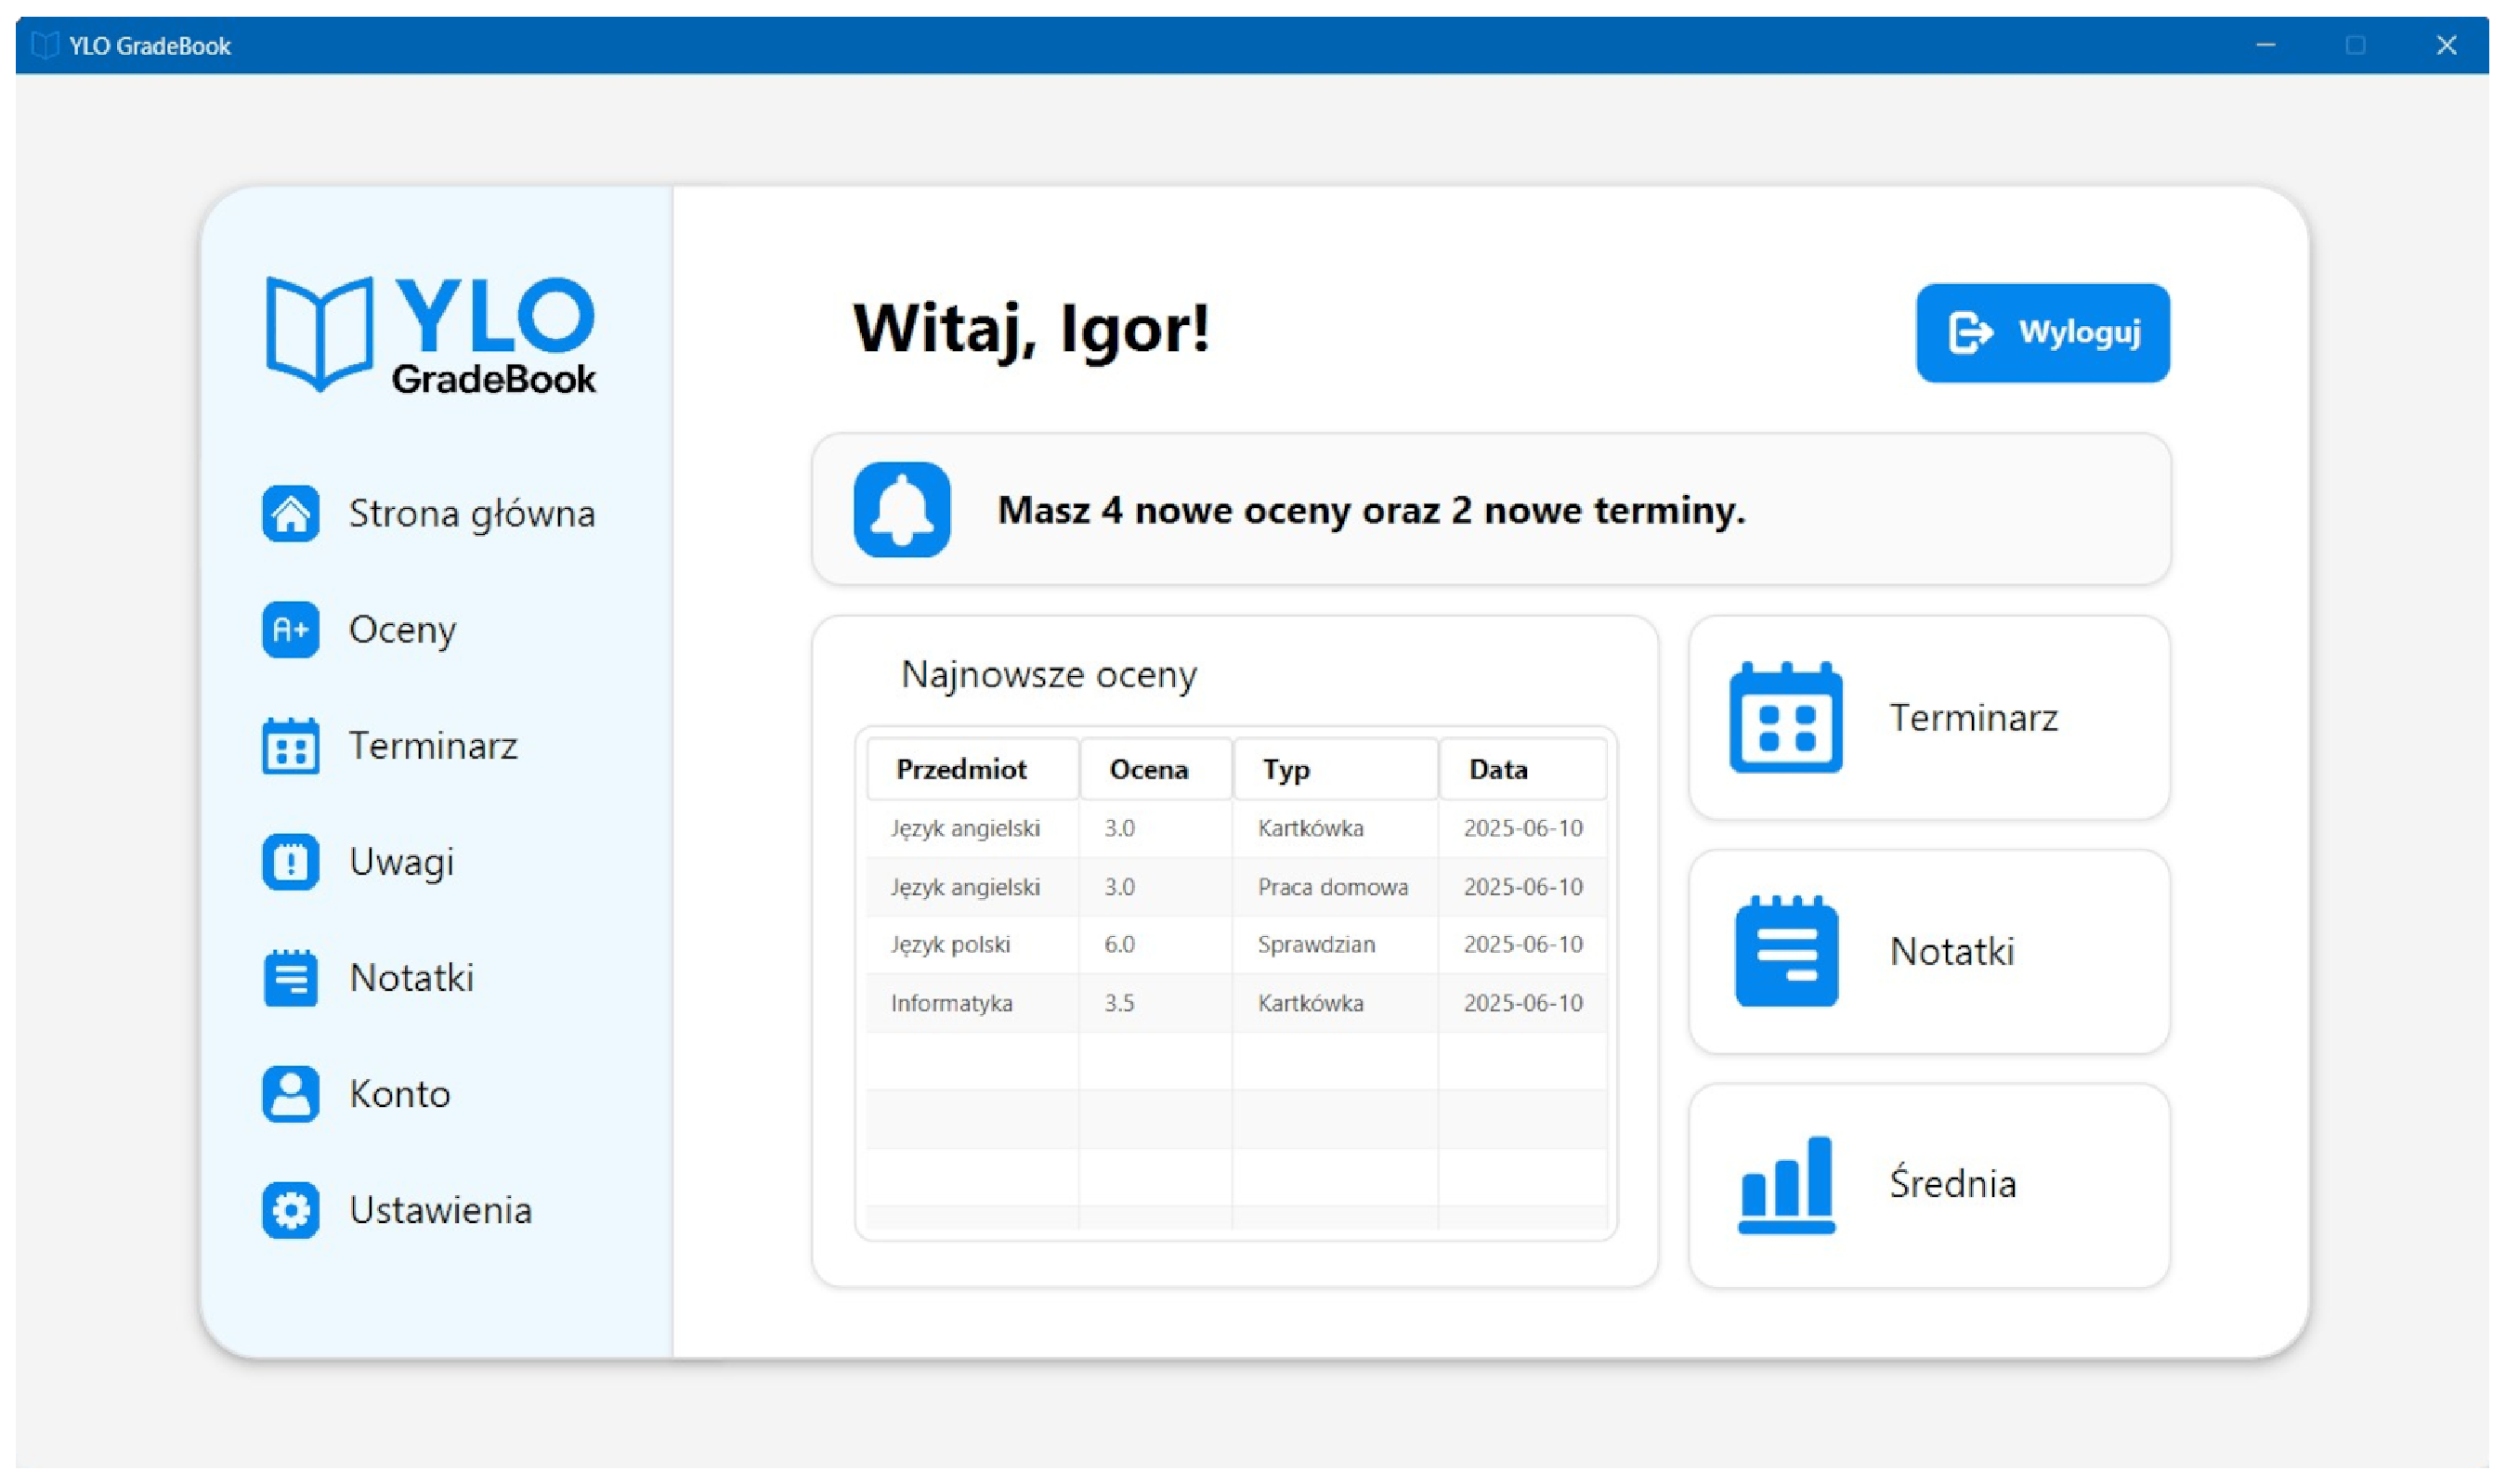
\includegraphics[width=0.9\textwidth]{figures/fig_0007.eps}
    \caption{Główny widok ucznia}
    \label{fig:studentWindow}
\end{figure}
\newpage
\subsubsection{Zakładka „Oceny”}
Widok ten umożliwia uczniowi przegląd ocen z podziałem na przedmioty oraz wyświetlenie średniej ocen z każdego z nich.
\begin{figure}[H]
    \centering
    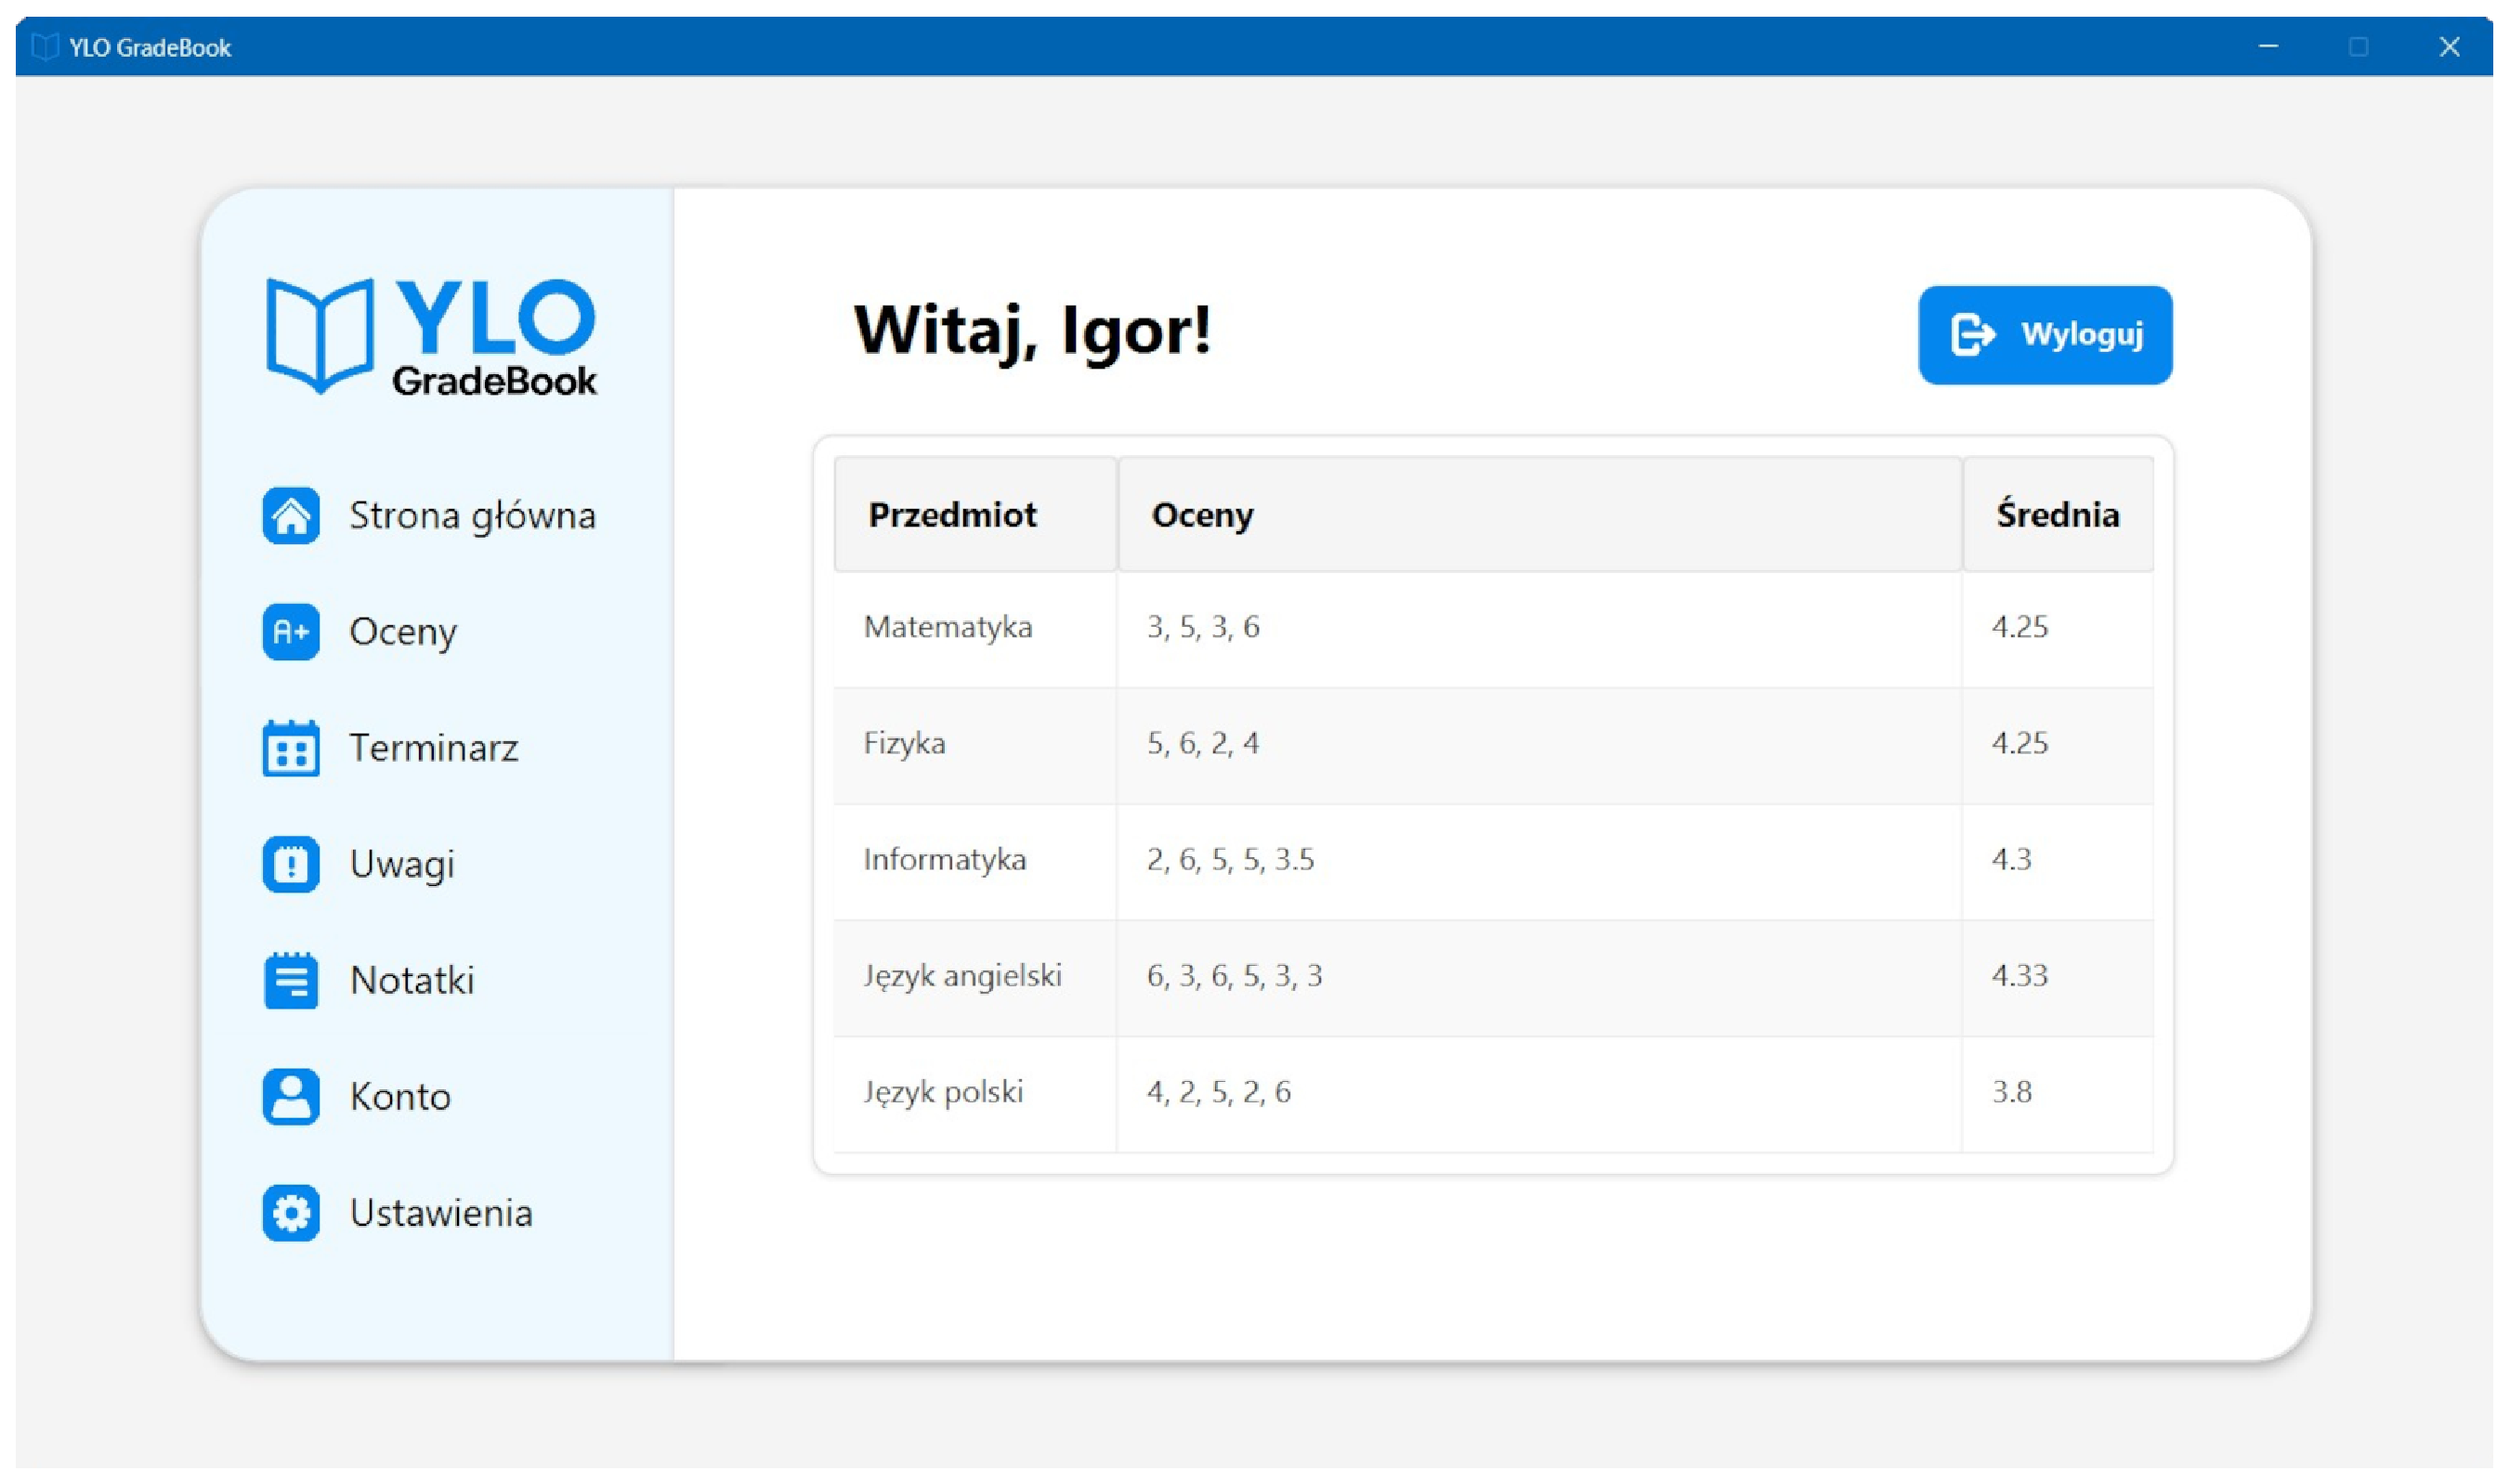
\includegraphics[width=0.9\textwidth]{figures/StudentWindow/fig_0009.eps}
    \caption{Okno ucznia - Zakładka „Oceny”}
    \label{fig:studentGradePane}
\end{figure}

\subsubsection{Zakładka „Terminarz”}
Zakładka służy do wyświetlania wszystkich nadchodzących terminów wydarzeń przypisanych do klasy ucznia.
\begin{figure}[H]
    \centering
    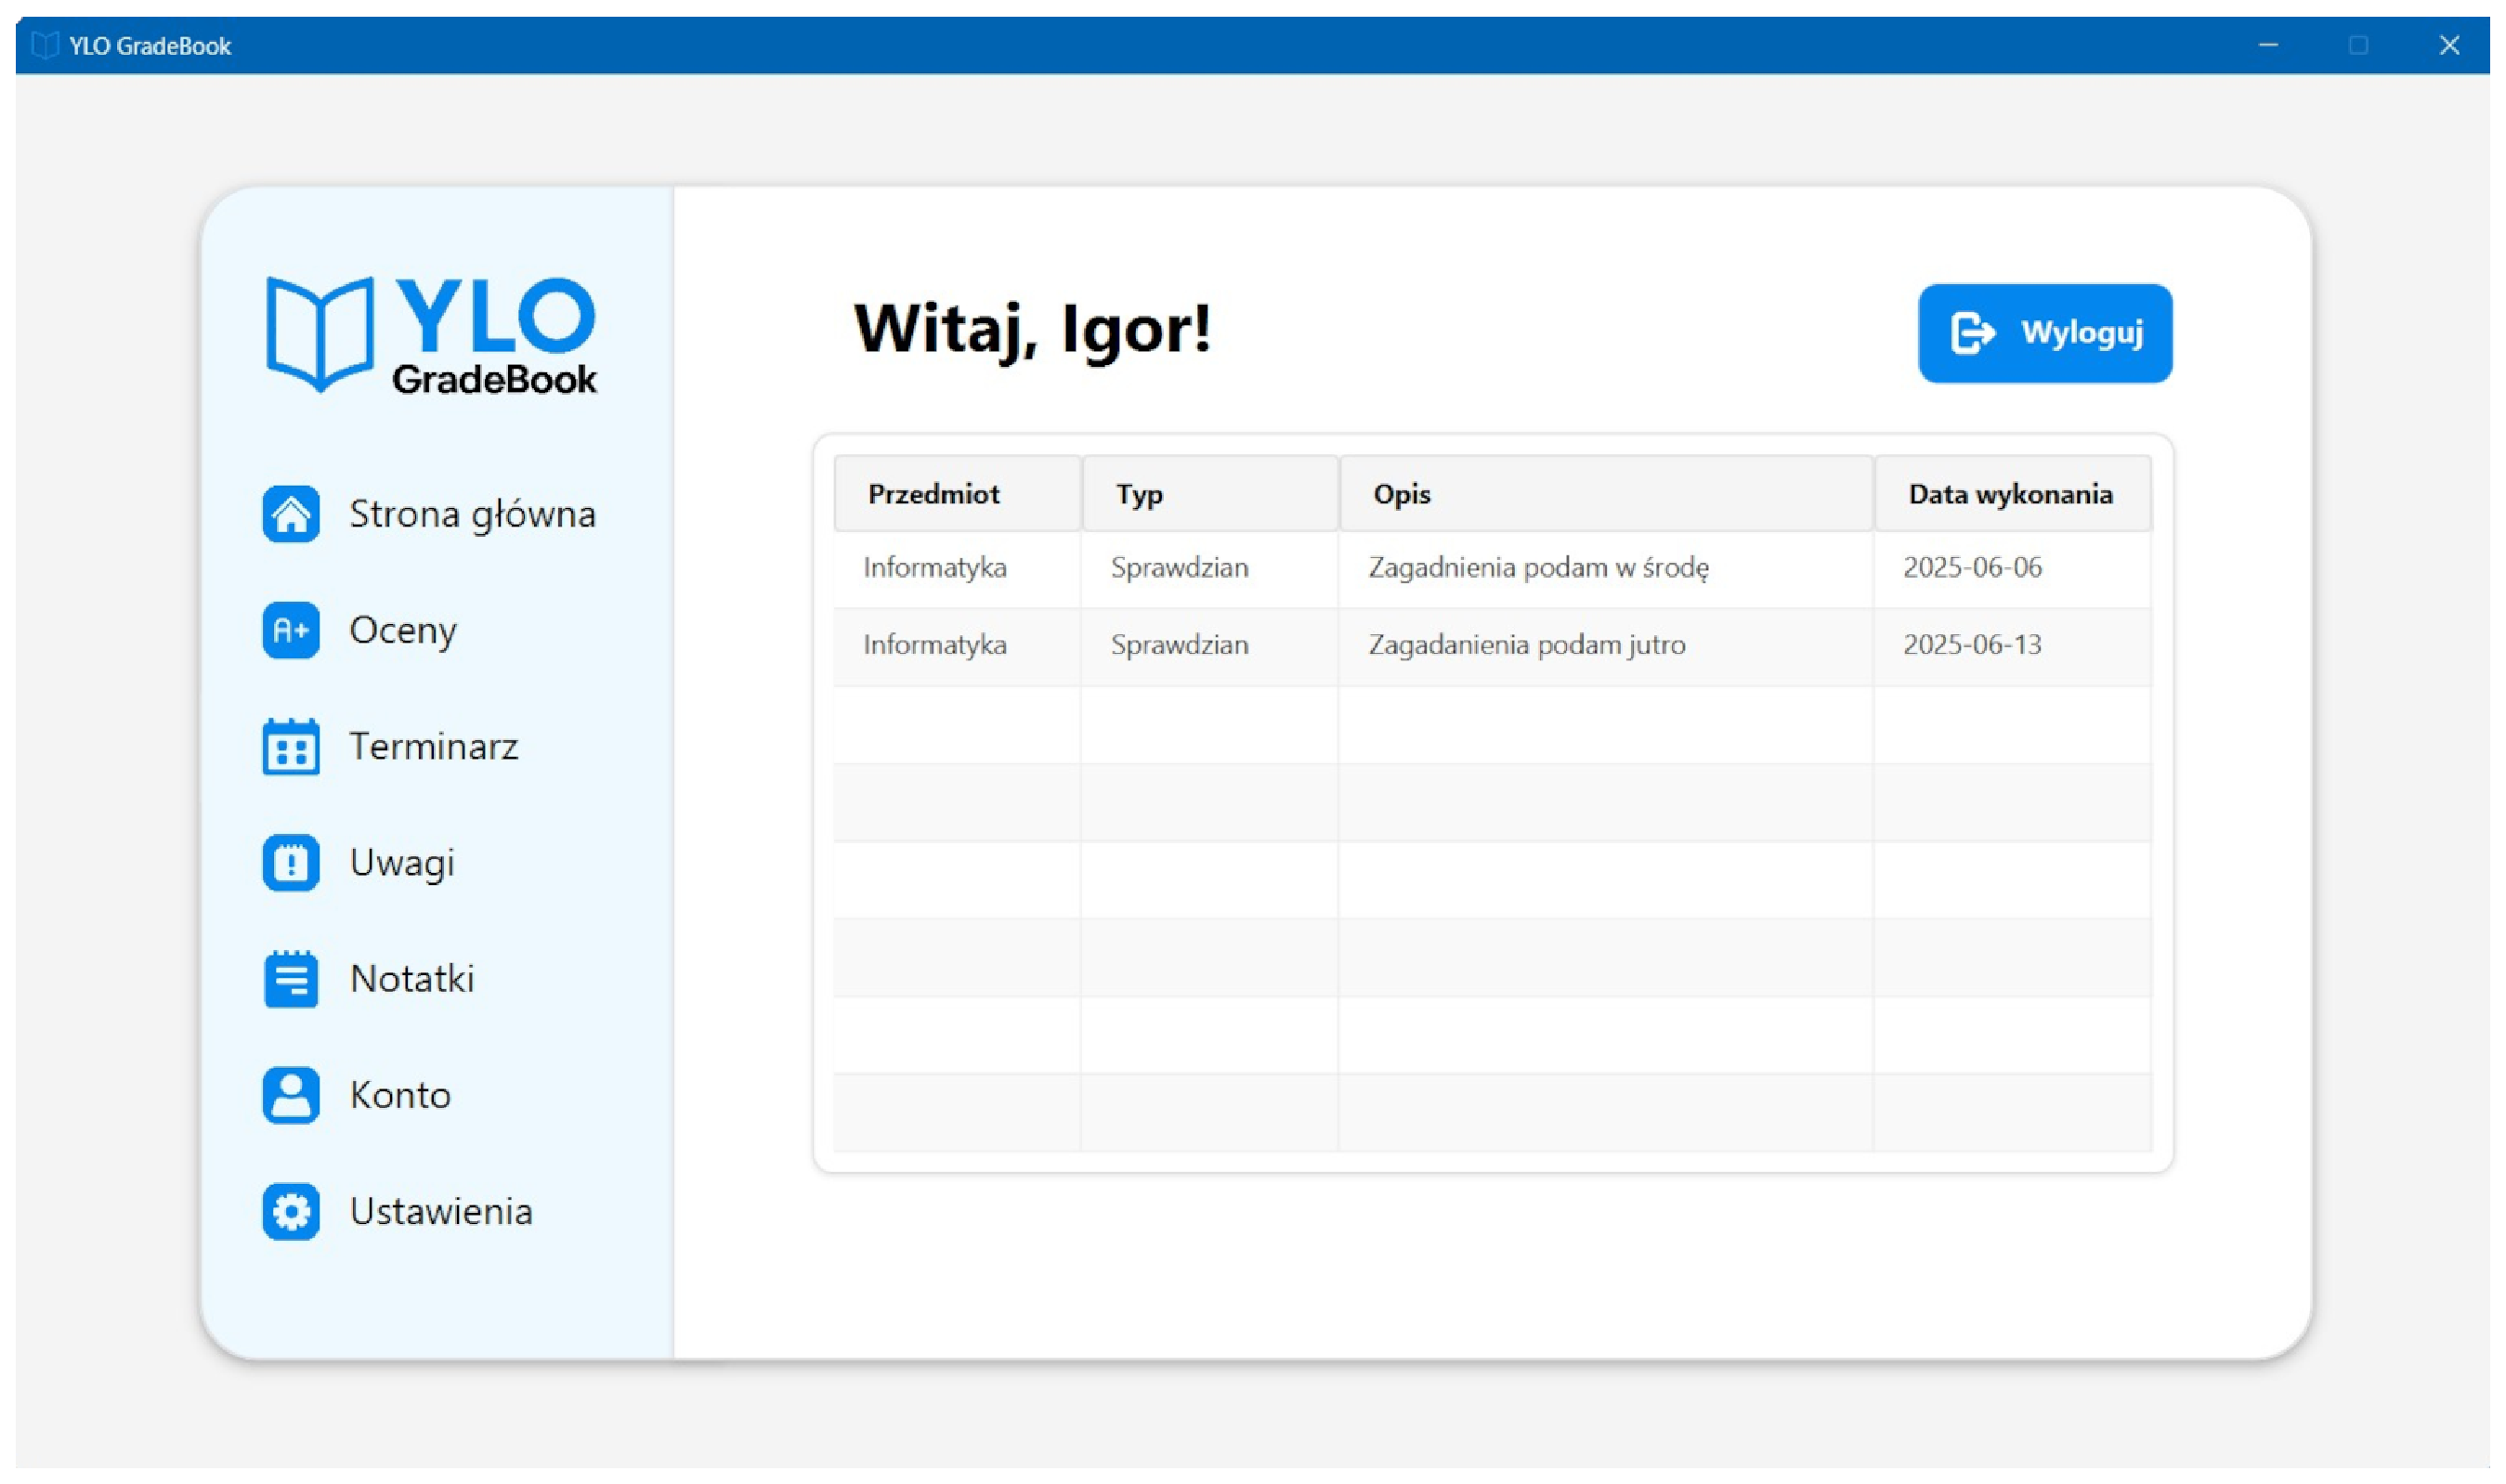
\includegraphics[width=0.9\textwidth]{figures/StudentWindow/fig_0010.eps}
    \caption{Okno ucznia - Zakładka „Terminarz”}
    \label{fig:studentDaedLinePane}
\end{figure}
\newpage
\subsubsection{Zakładka „Uwagi”}
Zakładka umożliwia przegląd uwag przypisanych do konta ucznia.
\begin{figure}[H]
    \centering
    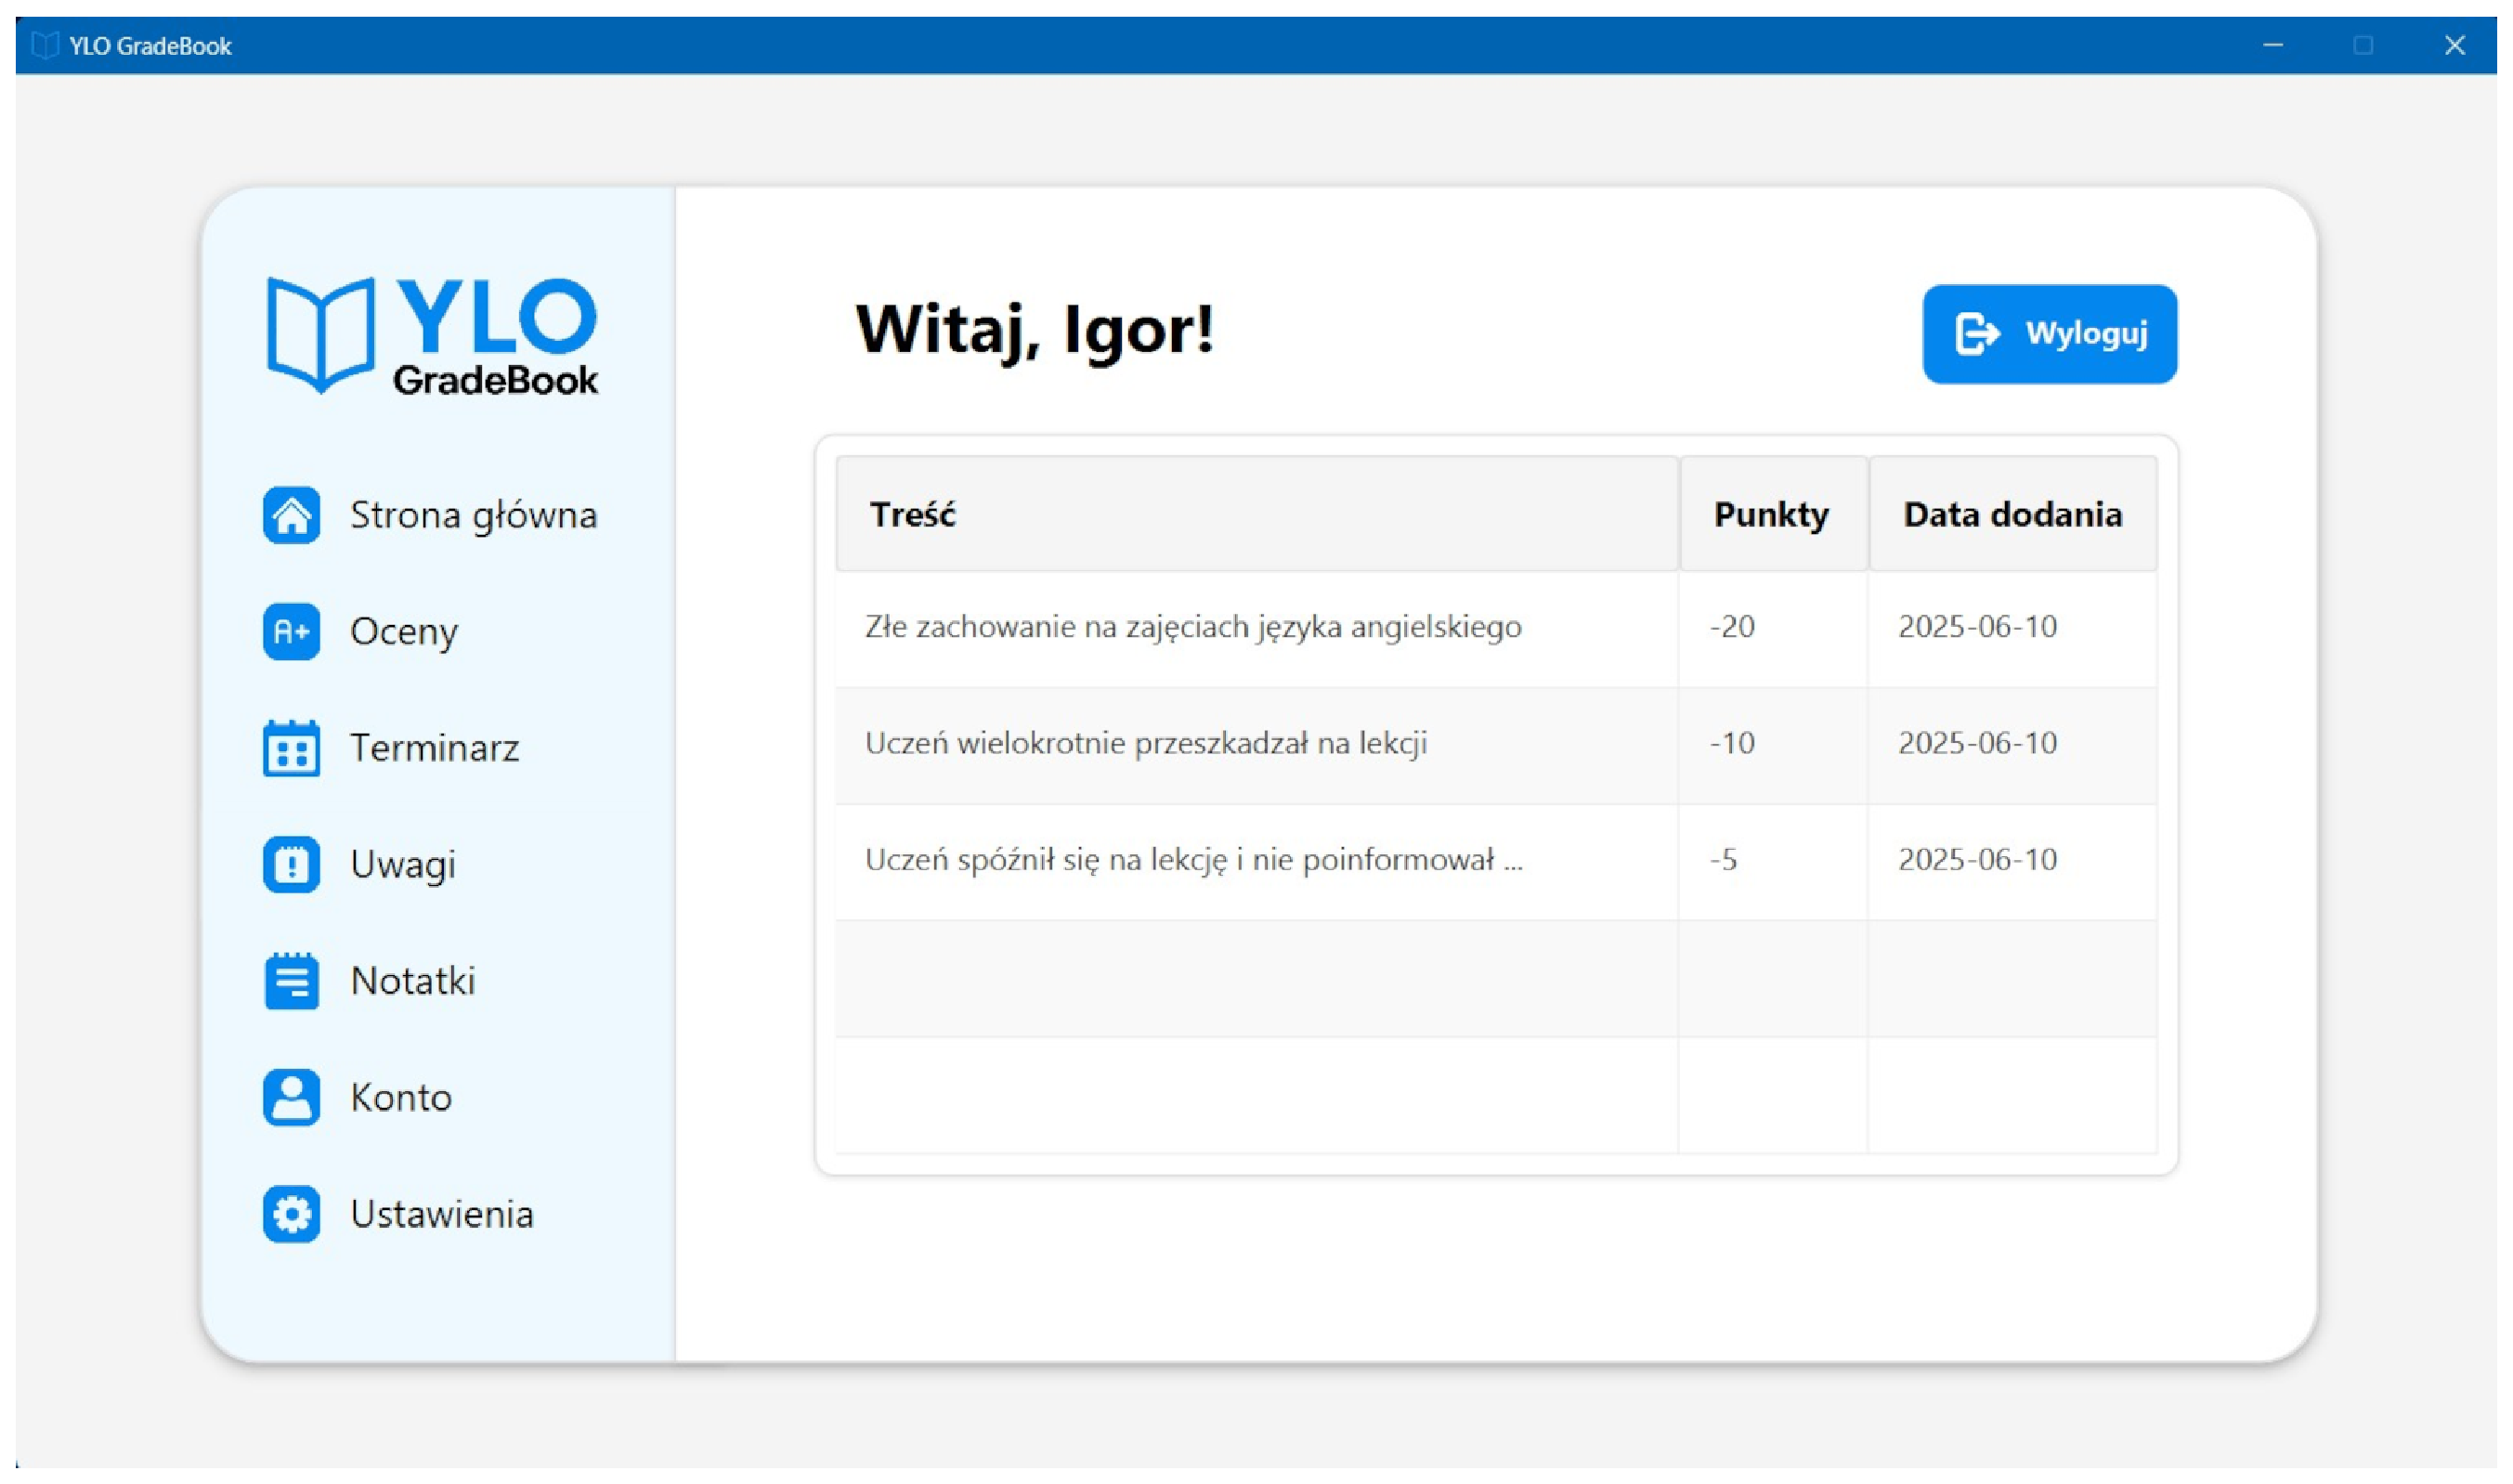
\includegraphics[width=0.9\textwidth]{figures/StudentWindow/fig_0011.eps}
    \caption{Okno ucznia - Zakładka „Uwagi”}
    \label{fig:studentNegativeNotesPane}
\end{figure}

\subsection*{Pozostałe zakładki}
Pozostałe zakładki zostaną zaprezentowane zbiorczo na końcu podrozdziału, ponieważ ich wygląd i funkcjonalność są identyczne niezależnie od przypisanej roli użytkownika
\newpage
\subsection{Główne okno interfejsu nauczyciela}
Główne okno interfejsu nauczyciela pojawia się bezpośrednio po jego zalogowaniu do systemu \texttt{YLO GradeBook}. Zostało zaprojektowane z myślą o szybkim i intuicyjnym dostępie do najważniejszych funkcji systemu. Podział treści na zakładki oraz wyraźna struktura interfejsu ułatwiają sprawne poruszanie się po aplikacji.
\begin{itemize}
    \item Po lewej stronie znajduje się panel nawigacyjny z zakładkami: \textbf{Strona główna}, \textbf{Oceny}, \textbf{Notatki}, \textbf{Konto} oraz \textbf{Ustawienia}.
    \item W górnej części widoku wyświetlane jest powitanie użytkownika wraz z jego imieniem, a także przycisk odpowiedzialny za kluczową funkcję — \textbf{dodawanie ocen}.
    \item Po prawej stronie umieszczono przycisk \textbf{Wyloguj}, umożliwiający szybkie zakończenie sesji.
    \item Centralna część okna prezentuje listę uczniów aktualnie wybranej klasy.
    \item Po prawej stronie znajdują się szybkie odnośniki do najczęściej wykonywanych operacji.
\end{itemize}

\begin{figure}[H]
    \centering
    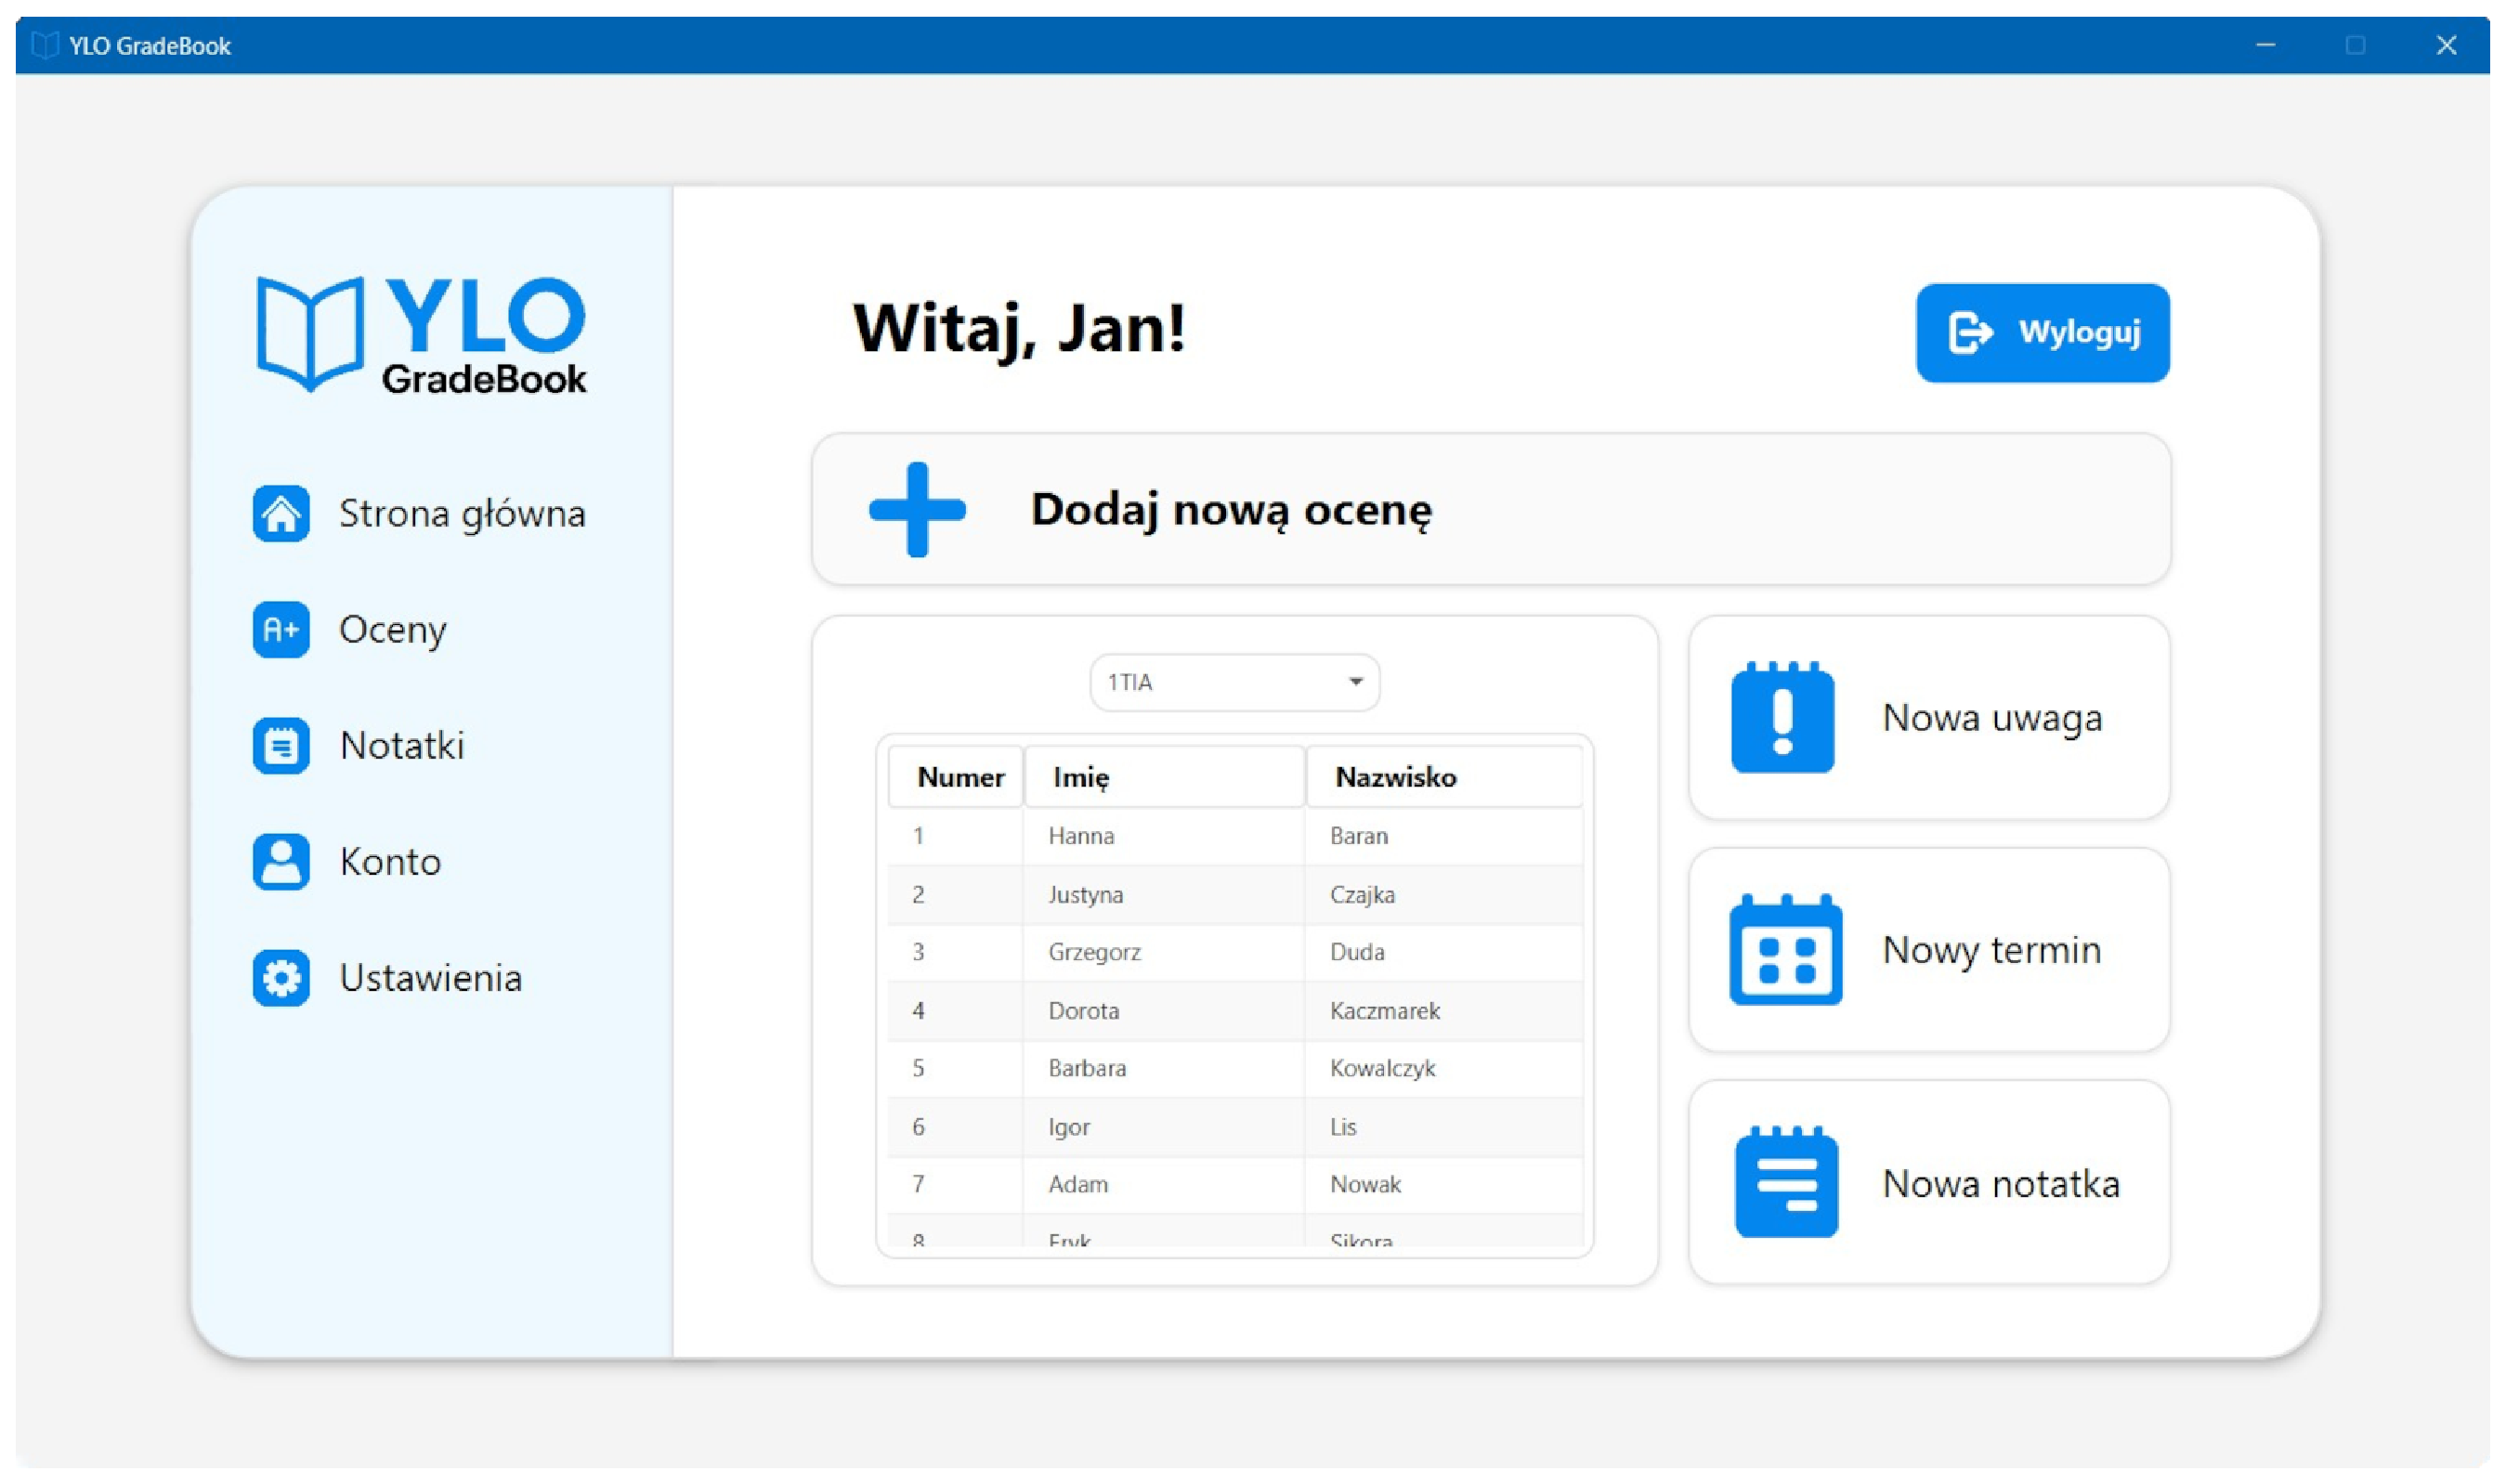
\includegraphics[width=0.9\textwidth]{figures/fig_0008.eps}
    \caption{Główny widok nauczyciela}
    \label{fig:teacherWindow}
\end{figure}
\newpage
\subsubsection{Zakładka „Oceny”}
Zakładka zawiera wyróżniony przycisk umożliwiający otwarcie okna typu pop-up, w którym nauczyciel może przypisać ocenę konkretnemu uczniowi.
Poniżej znajduje się tabela przedstawiająca oceny wszystkich uczniów wybranej klasy z danego przedmiotu.
\begin{figure}[H]
    \centering
    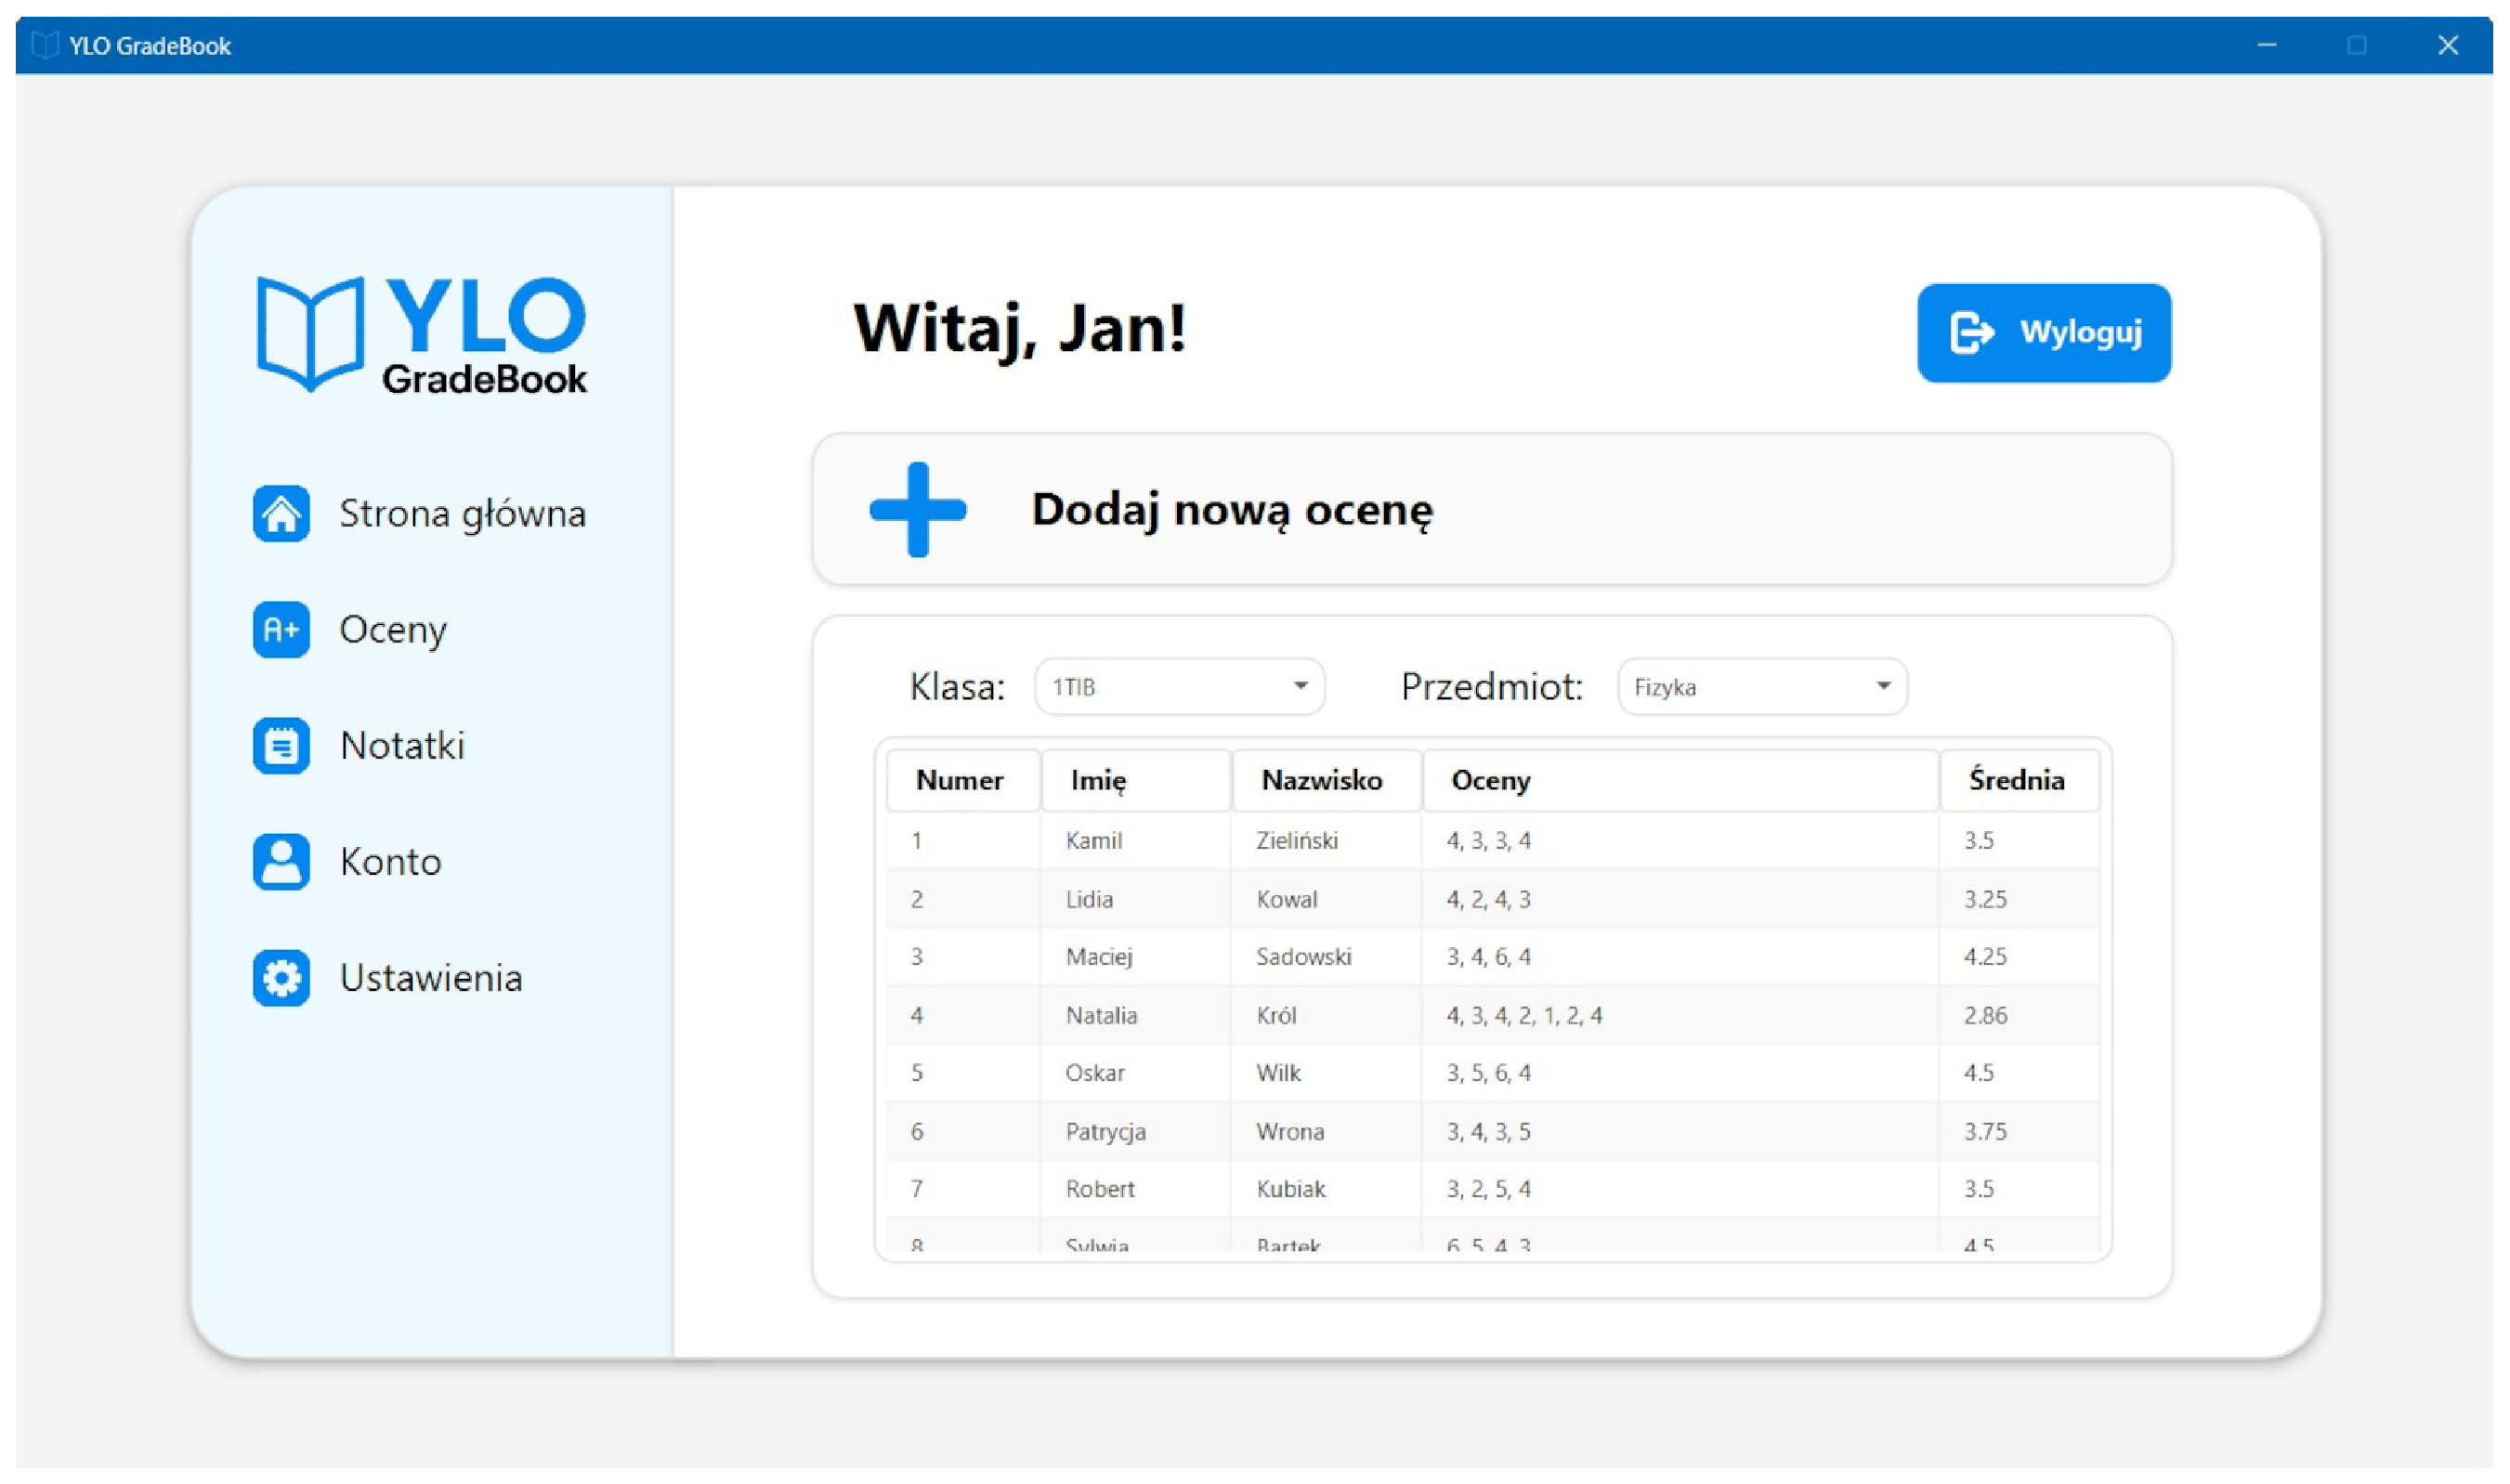
\includegraphics[width=0.9\textwidth]{figures/TeacherWindow/fig_0012.eps}
    \caption{Okno nauczyciela - Zakładka „Oceny”}
    \label{fig:teacherGradePane}
\end{figure}


\newpage
\subsection{Pozostałe zakładki}
Poniżej przedstawiono listę zakładek, które posiadają identyczną budowę, niezależnie od roli zalogowanego użytkownika.

\subsubsection{Zakładka „Notatki”}
Widok zawiera przycisk umożliwiający otwarcie okna typu pop-up, w którym użytkownik może dodać własną notatkę osobistą. Obok znajduje się również przycisk służący do odświeżania tabeli prezentującej wszystkie notatki przypisane do jego konta. Przy każdym rekodzie dodano przycisk textbf{Usuń}, który umożliwia usunięcie notatki z tabeli oraz z bazy danych.
\begin{figure}[H]
    \centering
    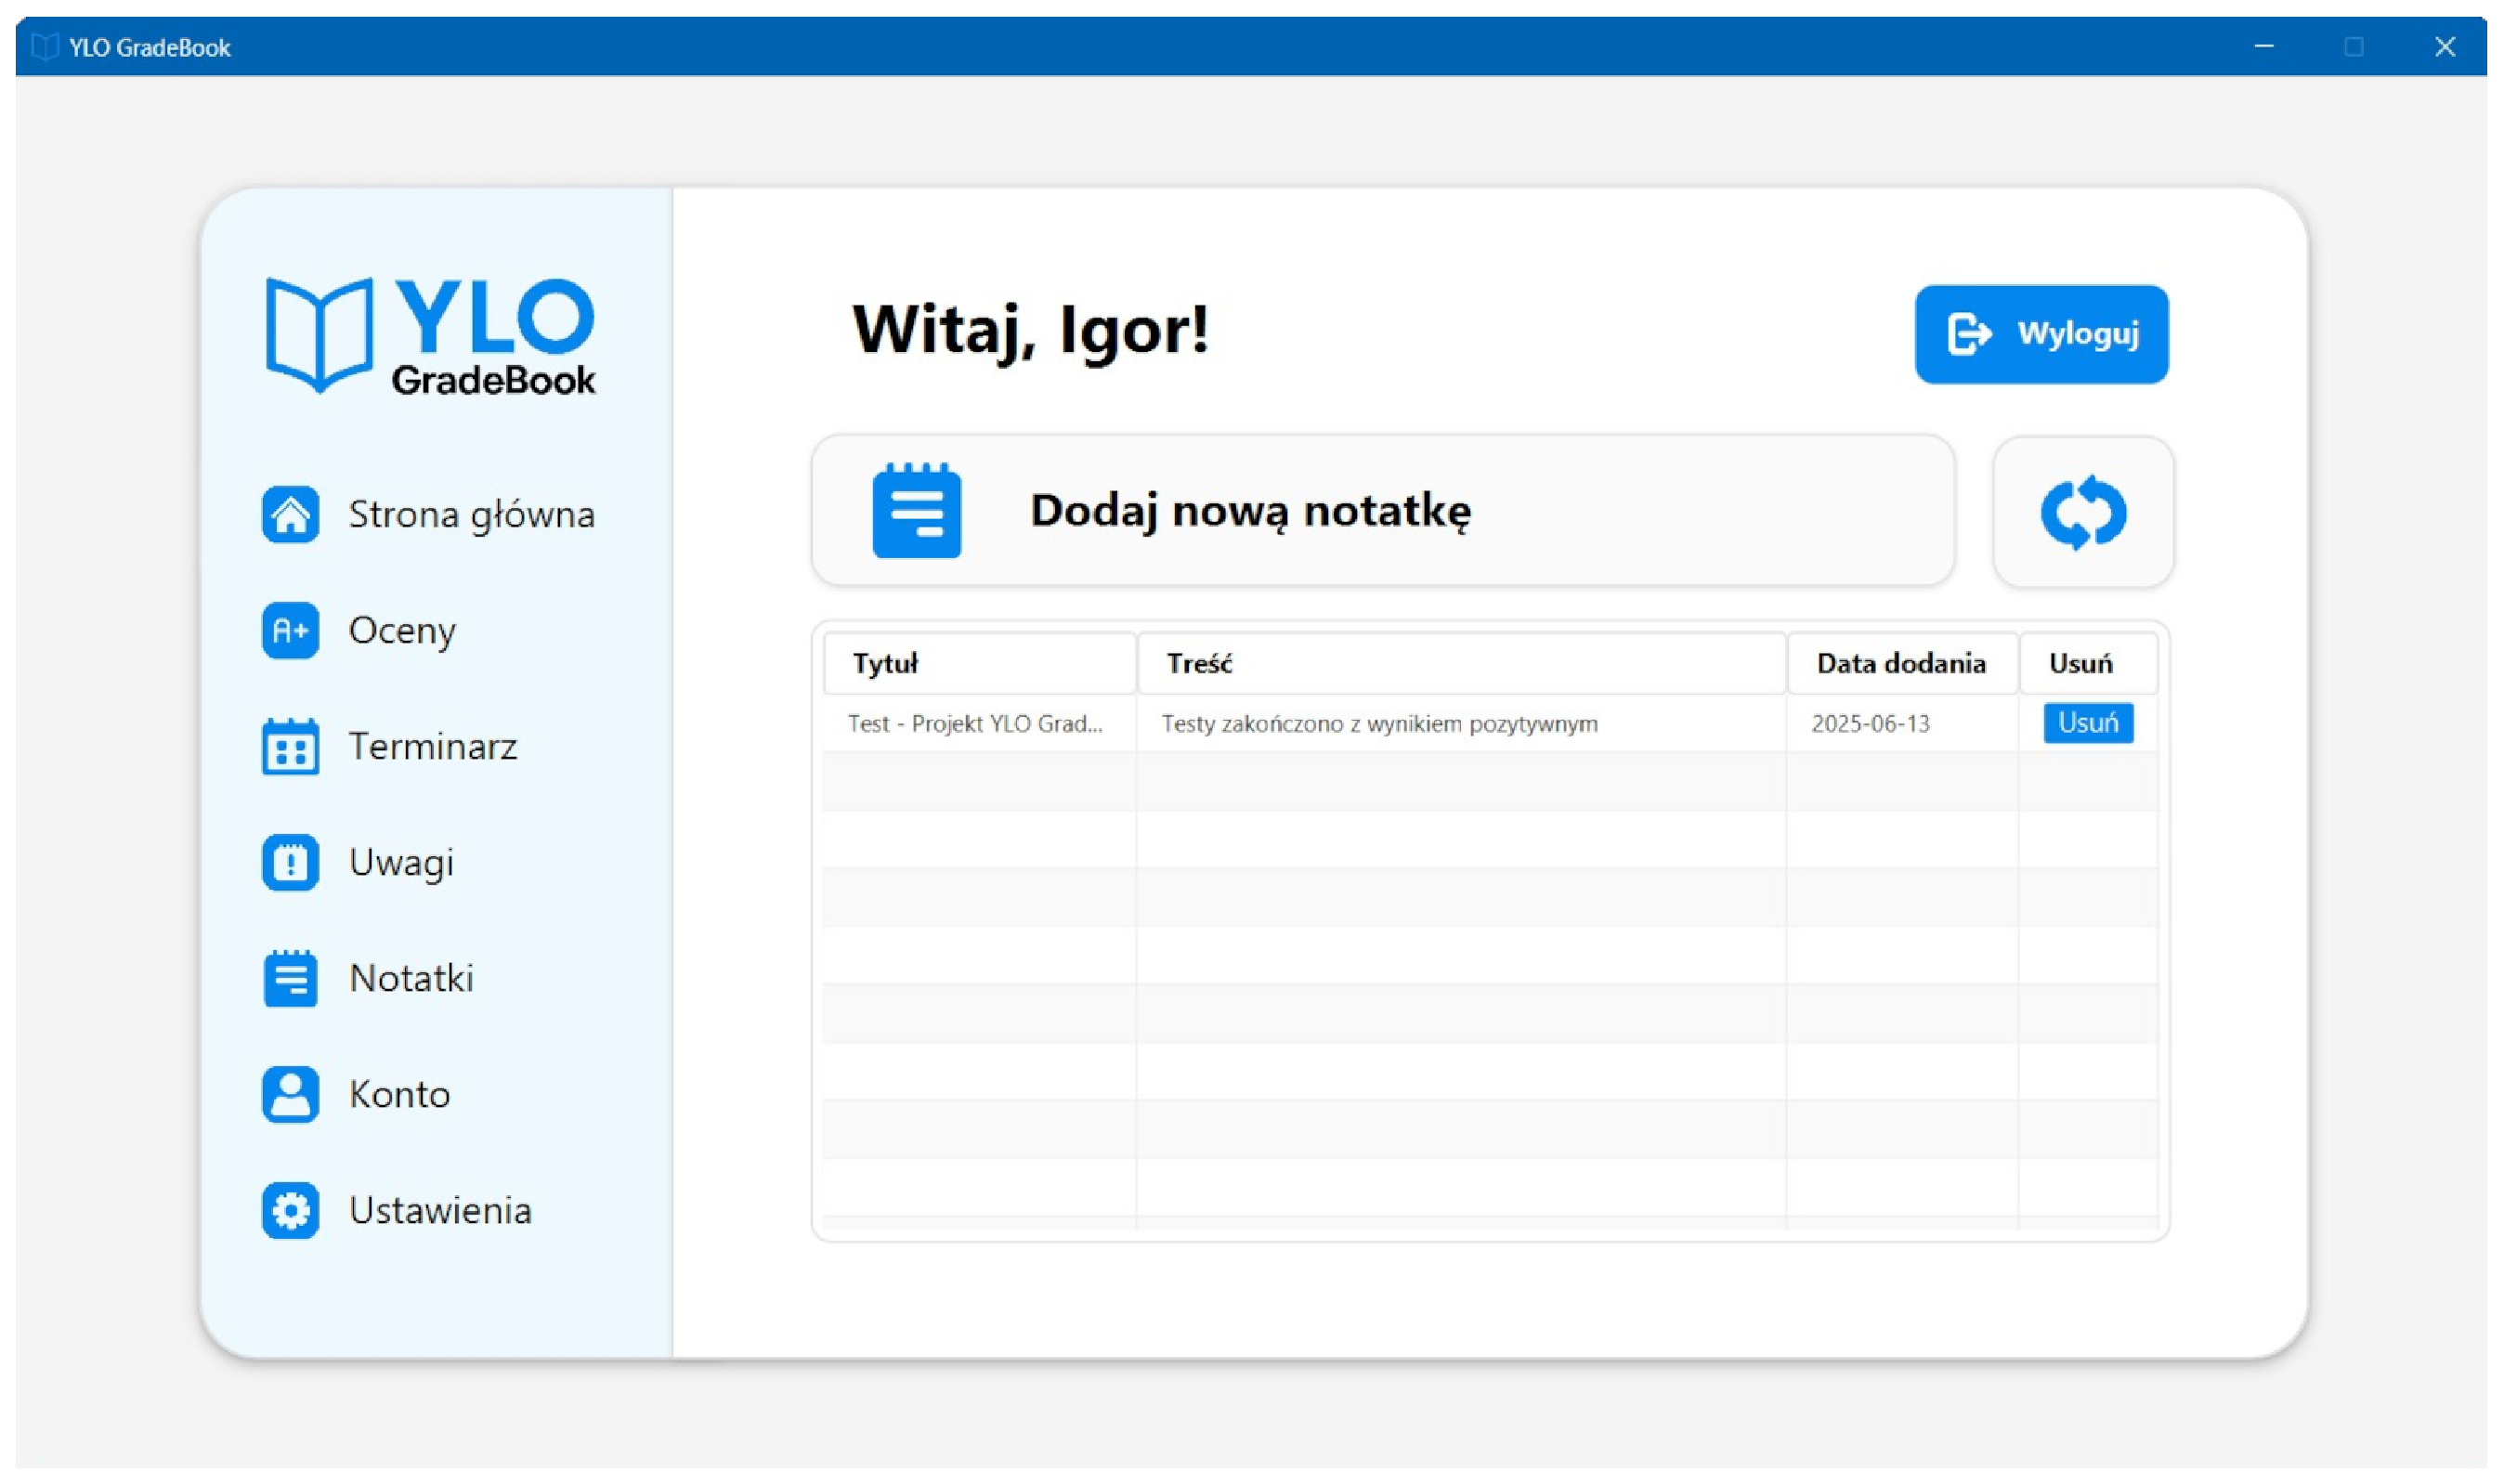
\includegraphics[width=0.9\textwidth]{figures/StudentWindow/fig_0013.eps}
    \caption{Okno ucznia - Zakładka „Notatki”}
    \label{fig:studentNotesPane}
\end{figure}
\newpage
\subsubsection{Zakładka „Konto”}
Widok pozwala na wyświetlenie danych użytkownika aktualnie zalogowanego do systemu.
\begin{figure}[H]
    \centering
    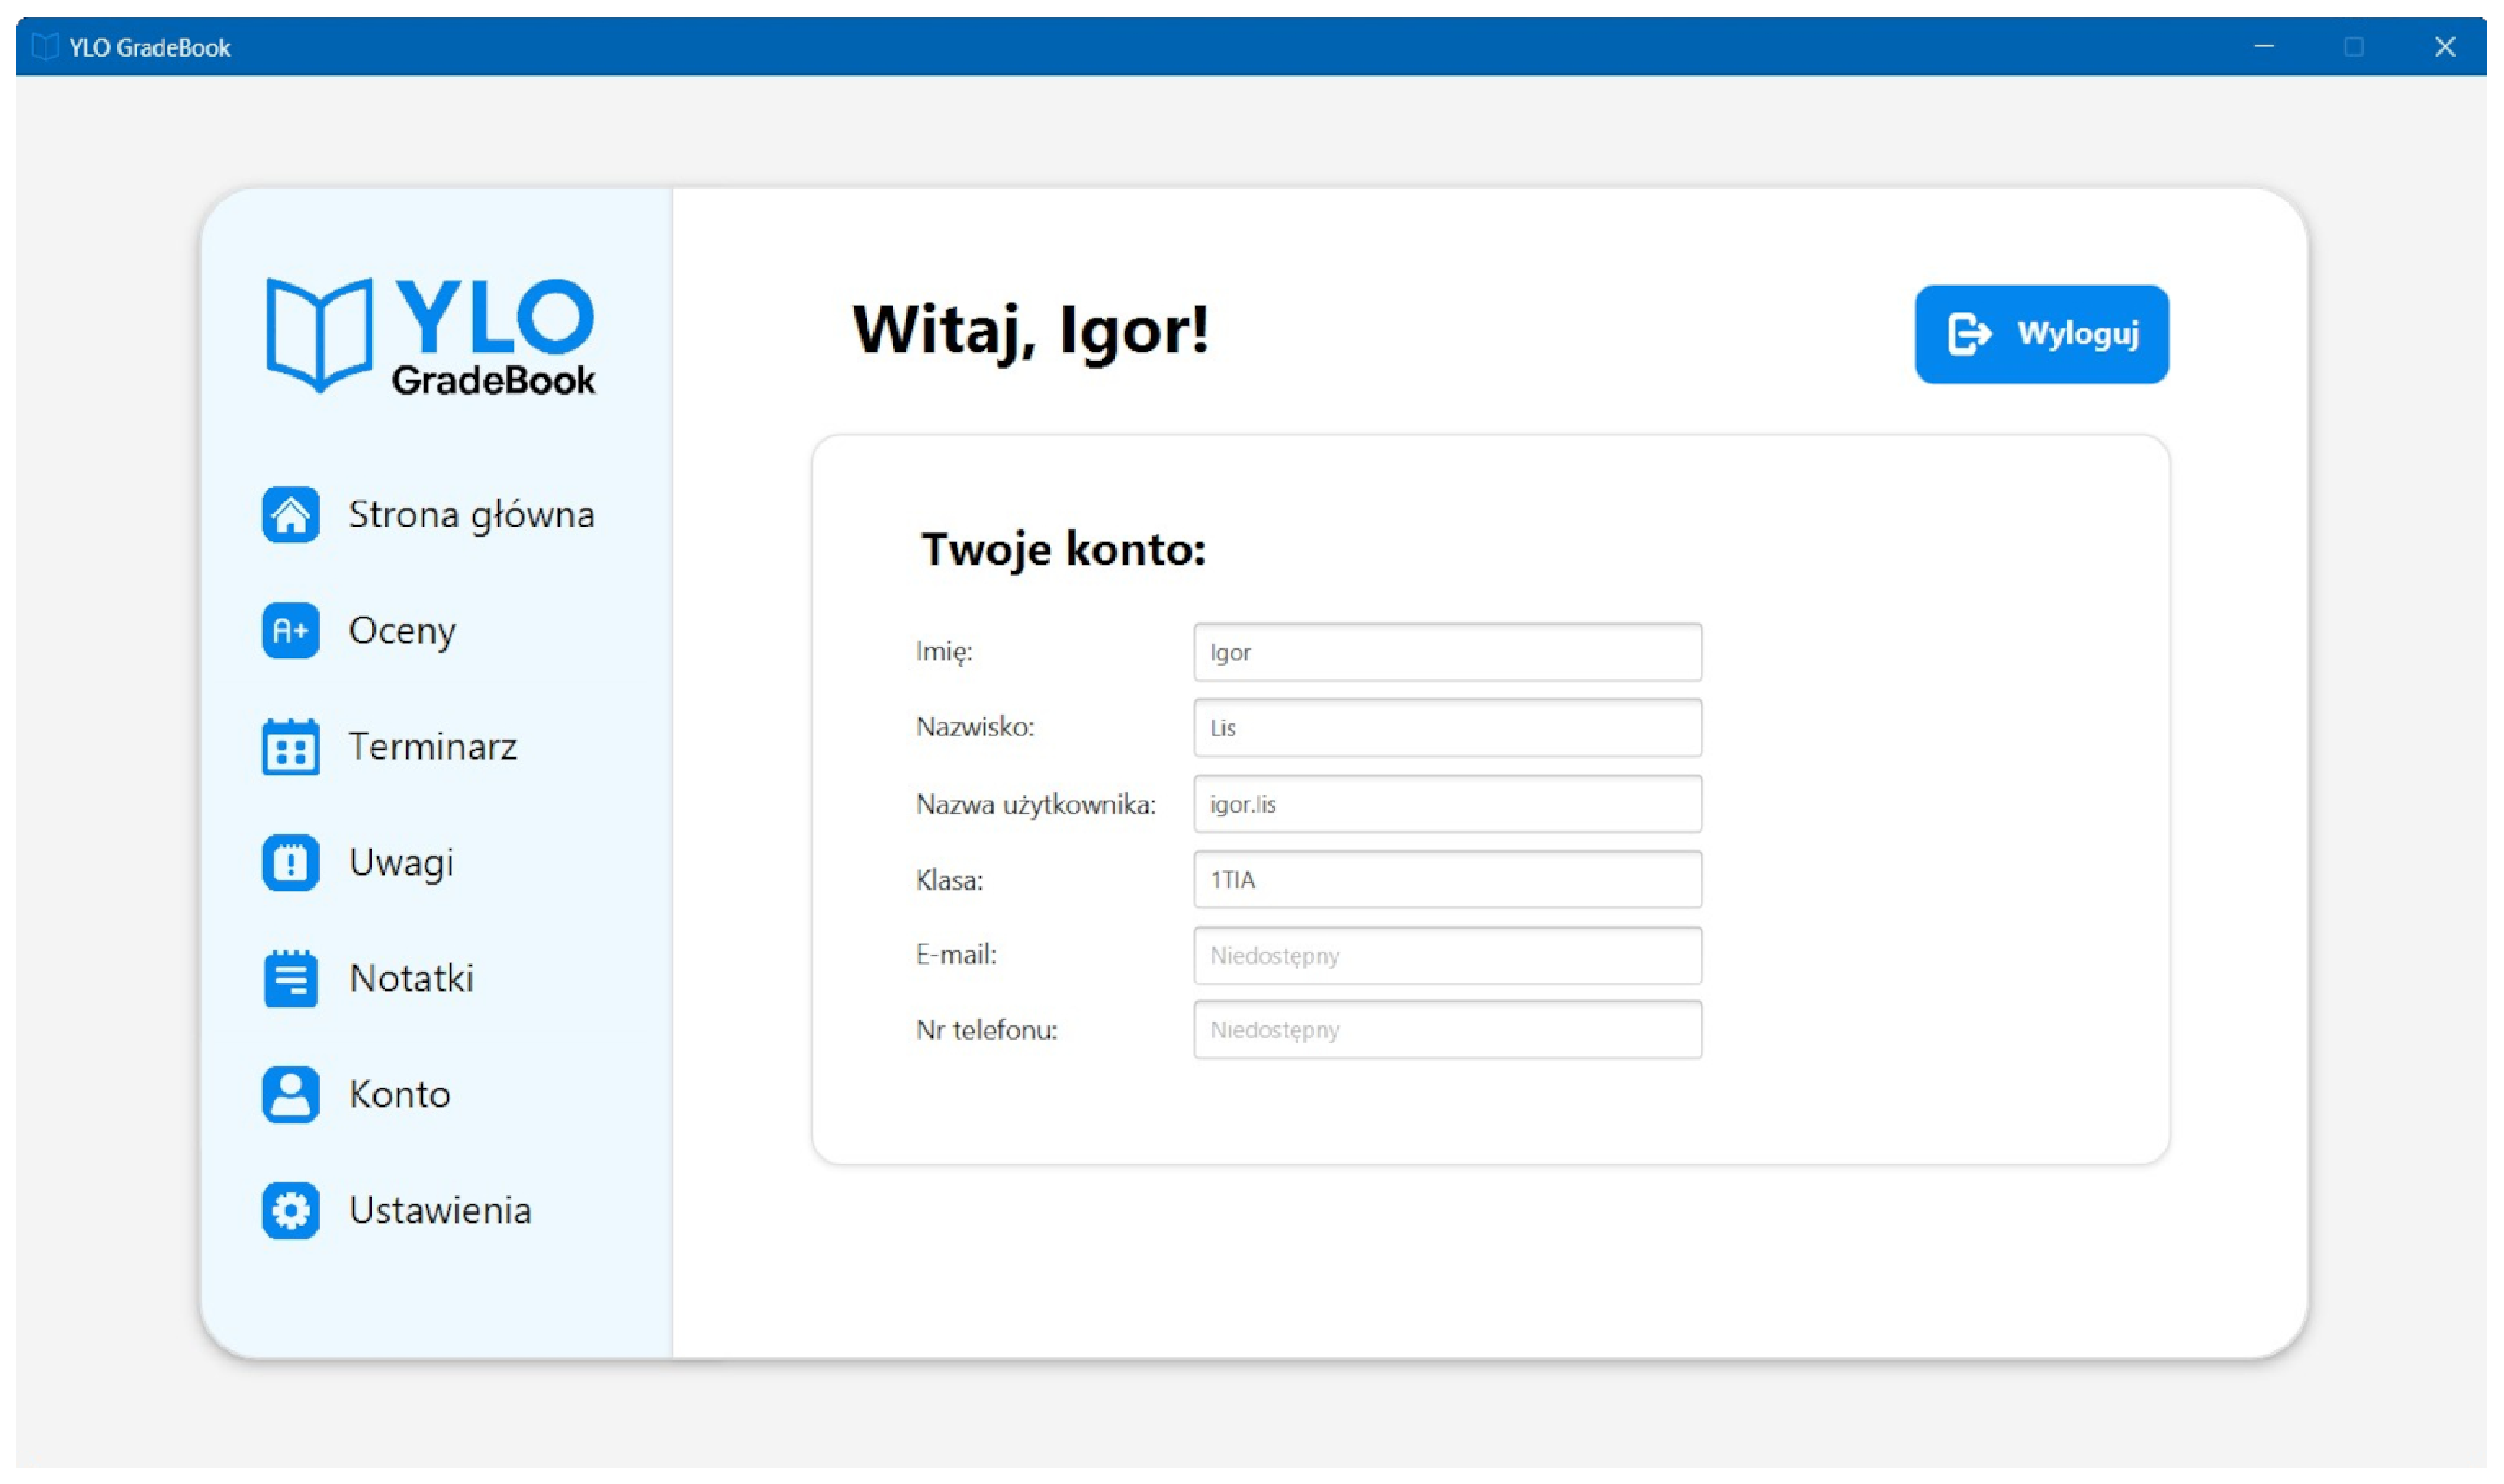
\includegraphics[width=0.9\textwidth]{figures/StudentWindow/fig_0014.eps}
    \caption{Zakładka „Konto”}
    \label{fig:accountPane}
\end{figure}

\subsubsection{Zakładka „Ustawienia”}
Ostatnia zakładka umożliwia użytkownikowi zarządzanie jego danymi konta. Zawiera przycisk uruchamiający okno resetowania hasła oraz przycisk przygotowany pod planowaną funkcję zmiany adresu e-mail przypisanego do profilu użytkownika.
\begin{figure}[H]
    \centering
    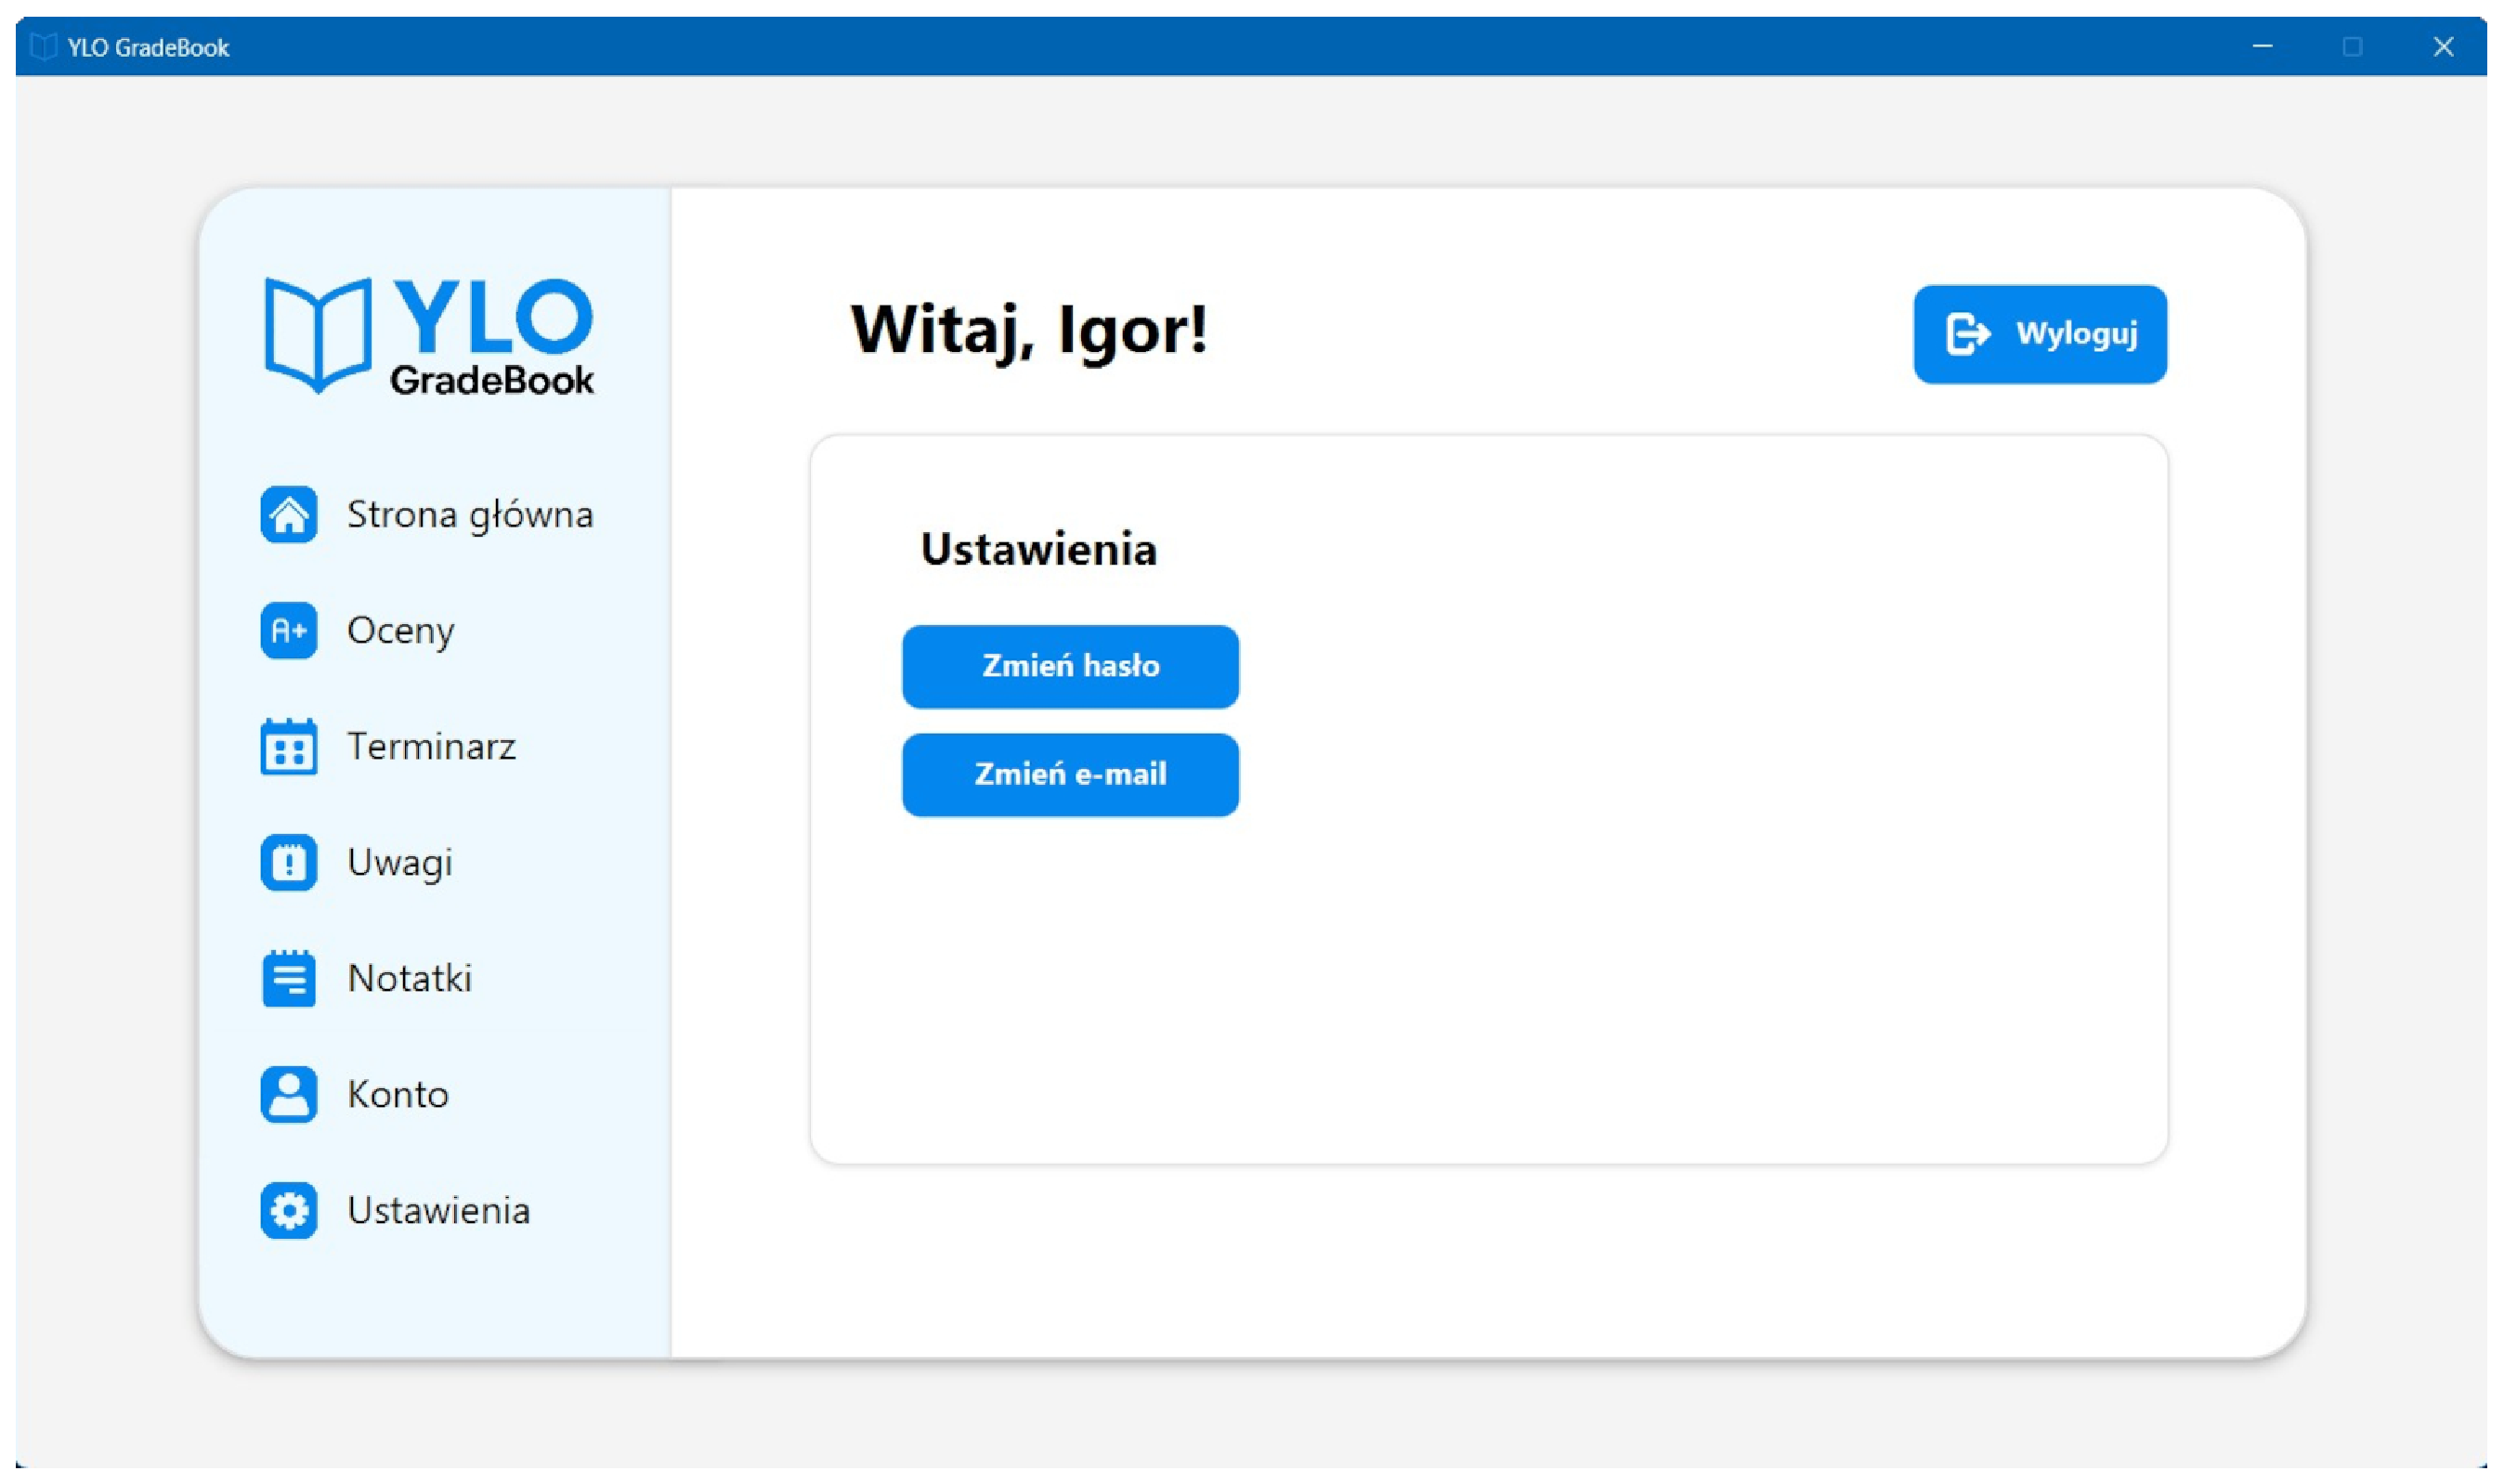
\includegraphics[width=0.9\textwidth]{figures/StudentWindow/fig_0015.eps}
    \caption{Zakładka „Ustawienia”}
    \label{fig:settingsPane}
\end{figure}

\subsection{Widok okna PopUp}
Widok ten służy do wyświetlenia formularza umożliwiającego dodanie nowych danych do systemu.
W zależności od kontekstu, posiada cztery różne wersje, z których każda odpowiada innej funkcji (np. dodawanie ocen, uwagi, terminu lub notatki).
\begin{itemize}
    \item Każda wersja zawiera pola do wprowadzania odpowiednich danych oraz przycisk umożliwiający dodanie ich do bazy danych.
    \item W przypadku błędnego wypełnienia formularza, system wyświetla odpowiedni komunikat walidacyjny.
    \item Po zatwierdzeniu formularza pojawia się komunikat informujący o rezultacie operacji — czy została wykonana pomyślnie, czy wystąpił błąd.
\end{itemize}
\clearpage

\subsubsection{Okno PopUp – Dodawanie oceny}

Formularz umożliwia nauczycielowi przypisanie nowej oceny wybranemu uczniowi. Widok zawiera listy rozwijane do wyboru klasy, ucznia, przedmiotu i typu oceny, a także pole do wpisania wartości punktowej.

\begin{figure}[H]
    \centering
    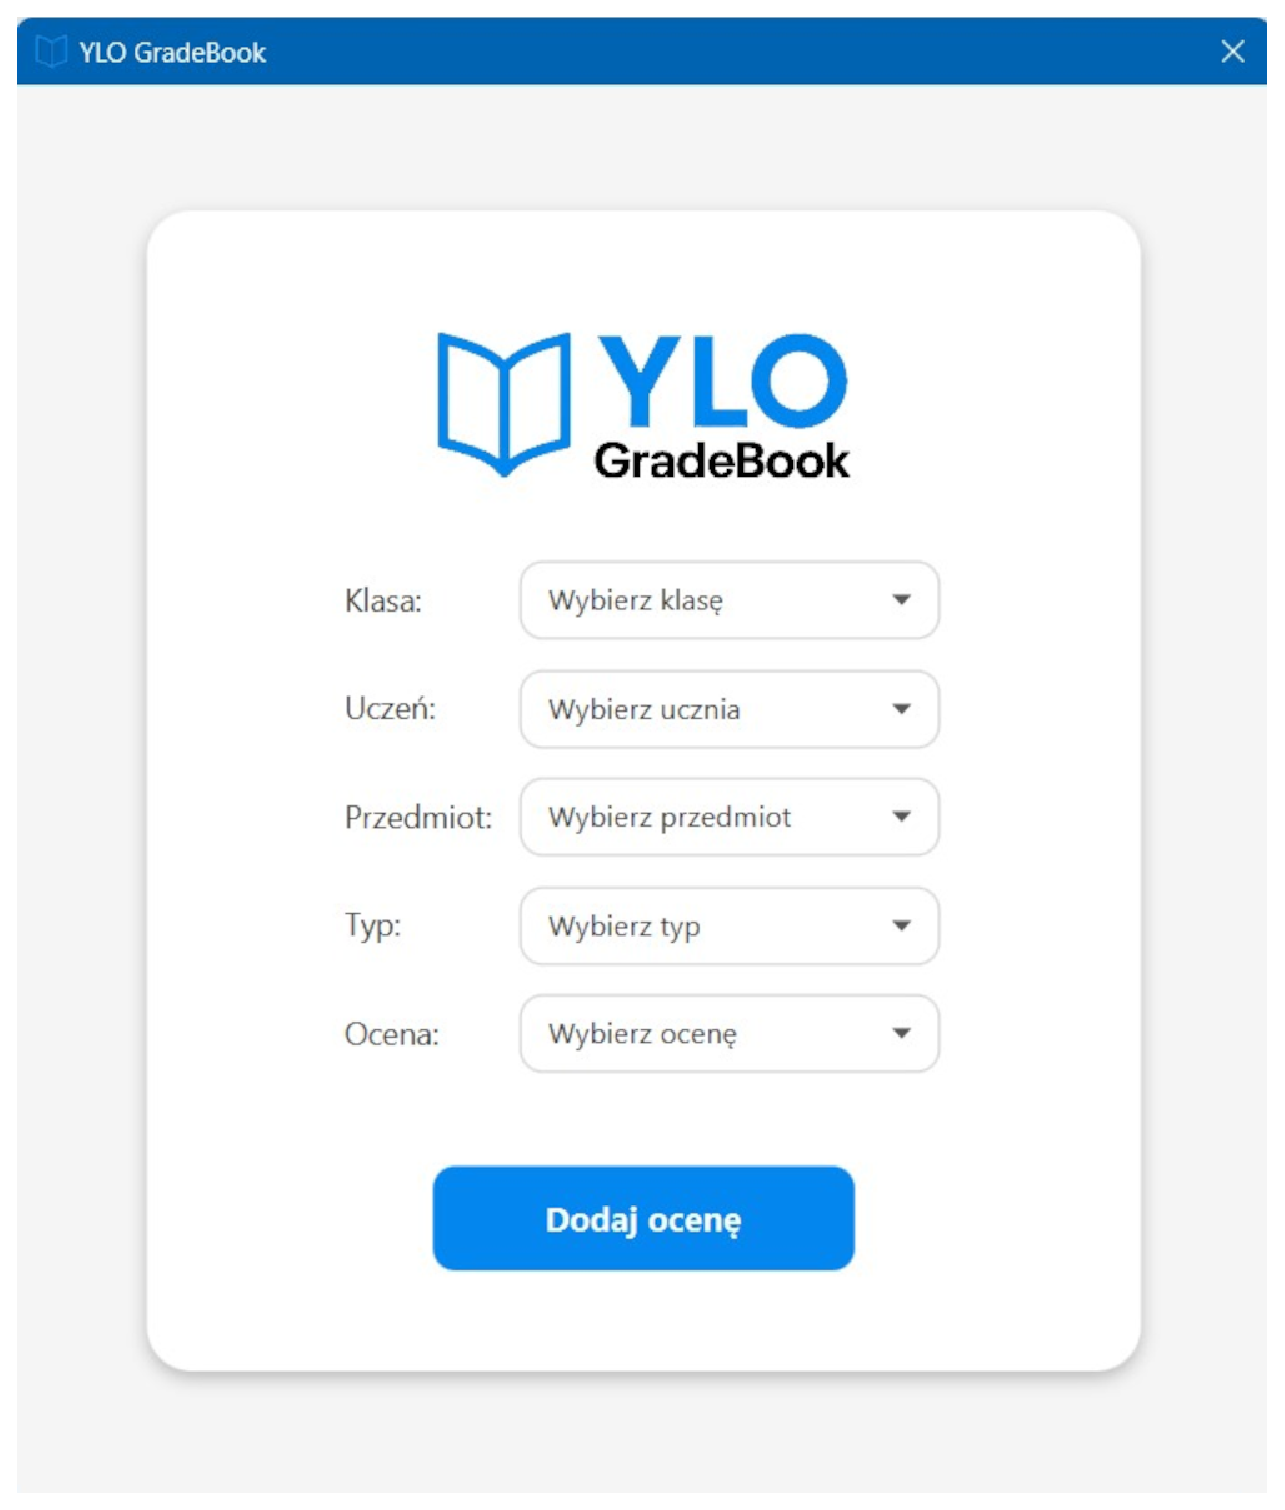
\includegraphics[width=0.9\textwidth]{figures/fig_0016.eps}
    \caption{PopUp — dodawanie nowej oceny}
    \label{fig:popUpGrade}
\end{figure}
\newpage
\subsubsection{Okno PopUp – Dodawanie terminów}

Okno to pozwala nauczycielowi na dodanie nowego wydarzenia (np. sprawdzianu, zadania) przypisanego do konkretnej klasy i przedmiotu. Użytkownik wybiera datę oraz podaje krótki opis.

\begin{figure}[H]
    \centering
    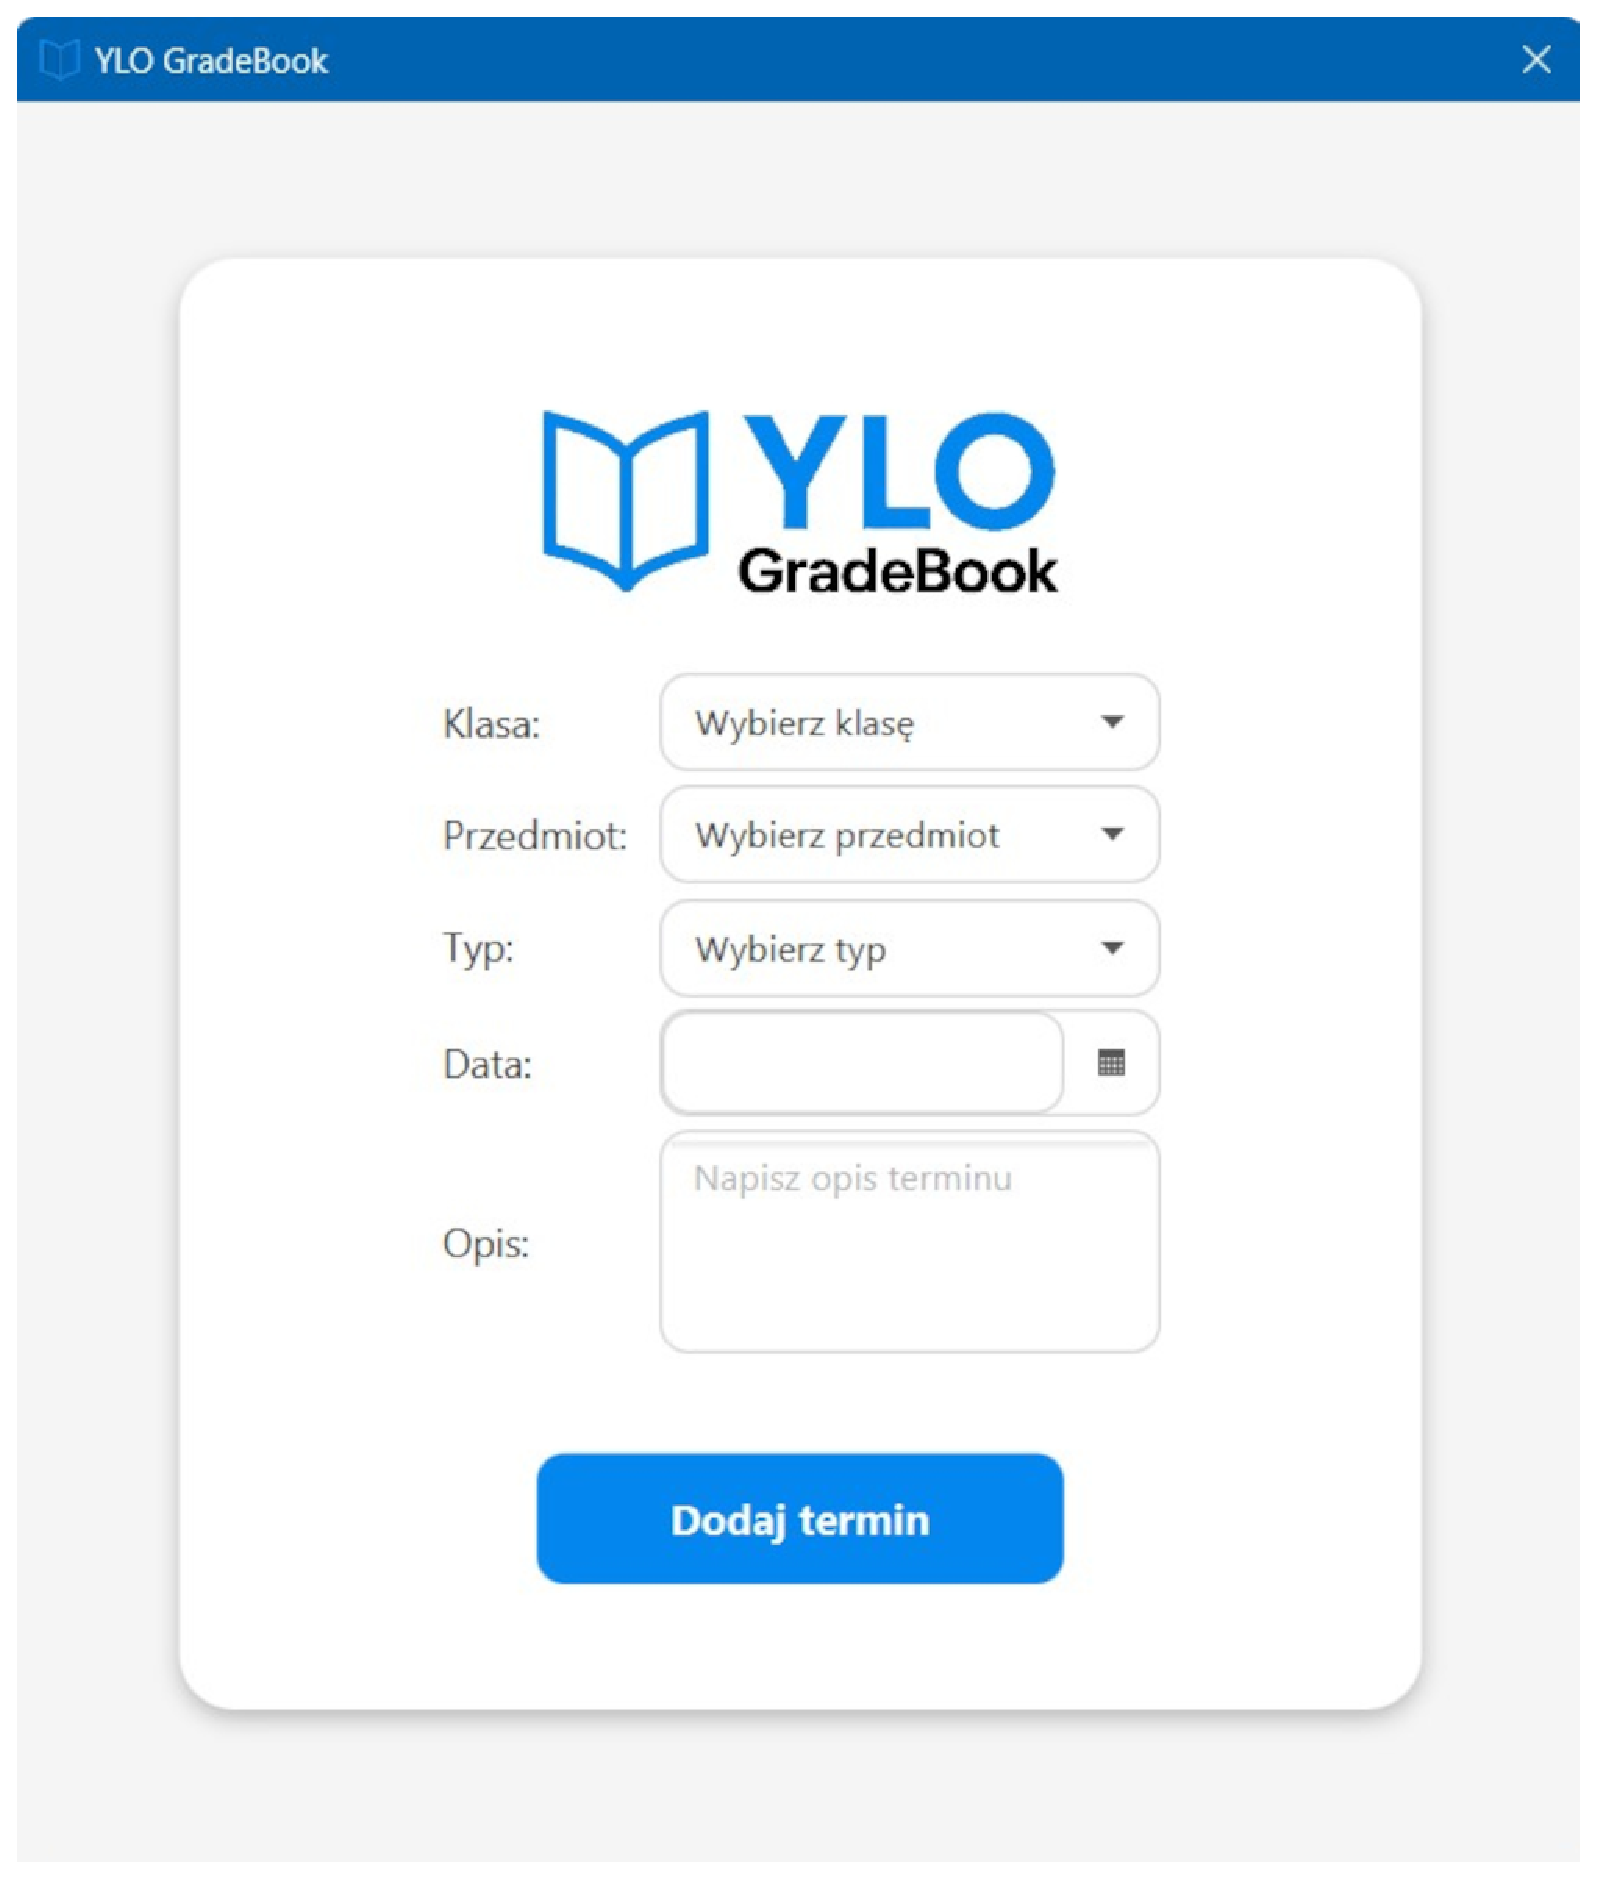
\includegraphics[width=0.9\textwidth]{figures/fig_0017.eps}
    \caption{PopUp — dodawanie nowego terminu}
    \label{fig:popUpDeadLine}
\end{figure}
\newpage
\subsubsection{Okno PopUp – Dodawanie uwag}

Formularz służy do wystawiania uwag punktowych uczniom. Nauczyciel wybiera ucznia, wprowadza liczbę punktów oraz wpisuje treść ograniczoną do 60 znaków.

\begin{figure}[H]
    \centering
    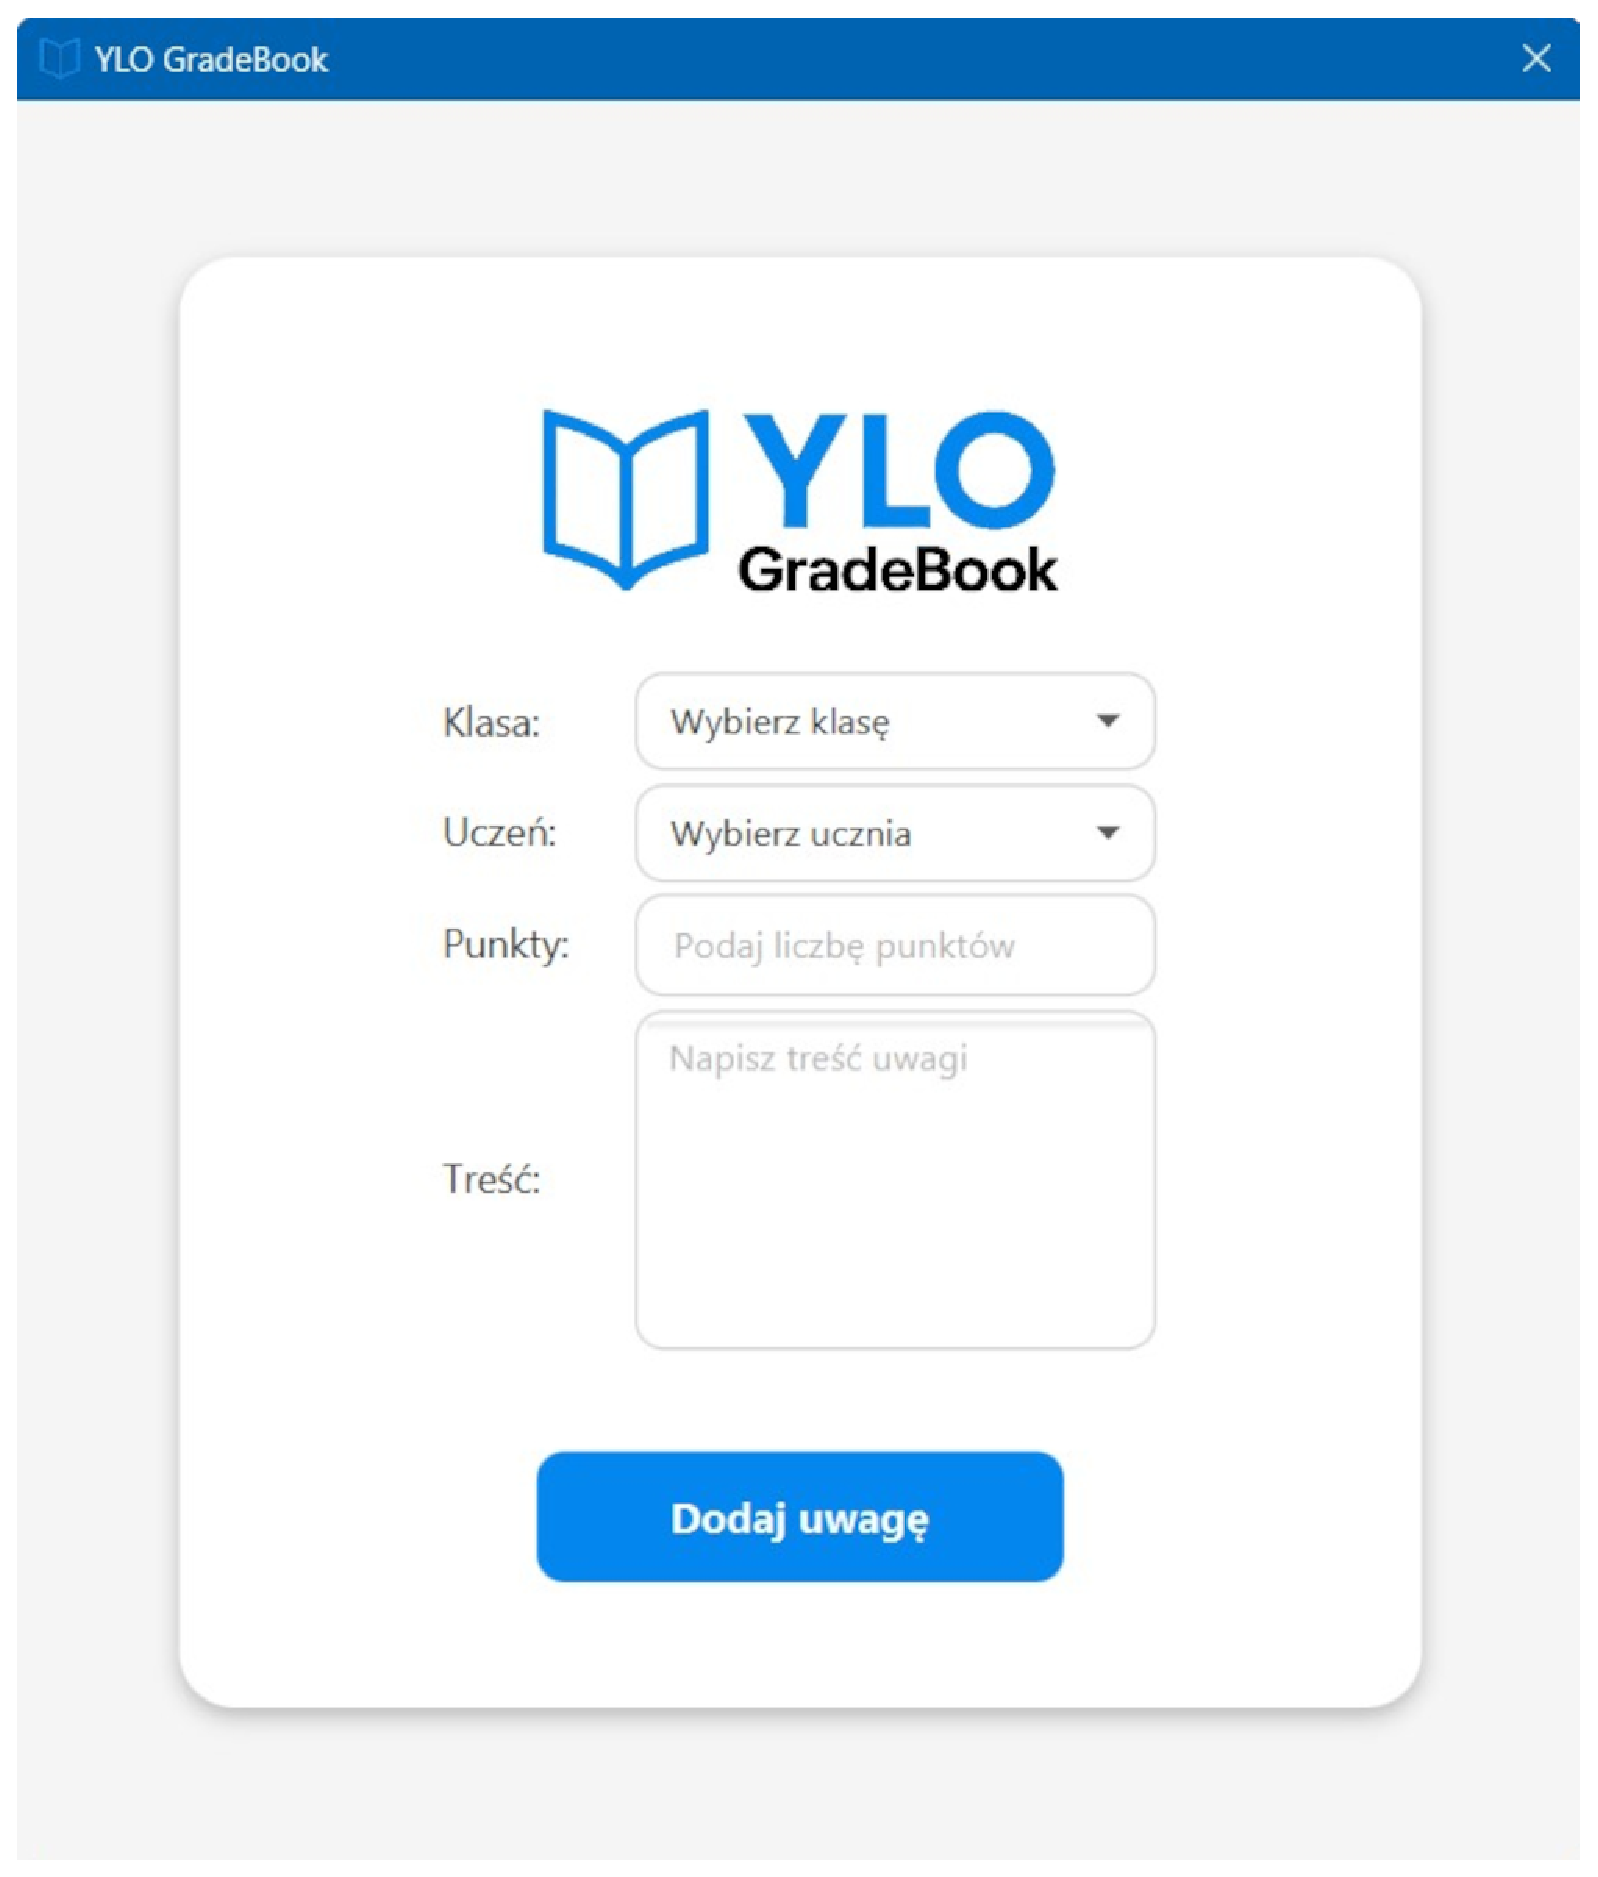
\includegraphics[width=0.9\textwidth]{figures/fig_0018.eps}
    \caption{PopUp — dodawanie uwagi uczniowi}
    \label{fig:popUpNN}
\end{figure}
\newpage
\subsubsection{Okno PopUp – Dodawanie notatek}
Widok umożliwia dodanie osobistej notatki. Użytkownik podaje tytuł oraz treść, a następnie zapisuje ją w systemie — notatka przypisywana jest automatycznie do jego konta.

\begin{figure}[H]
    \centering
    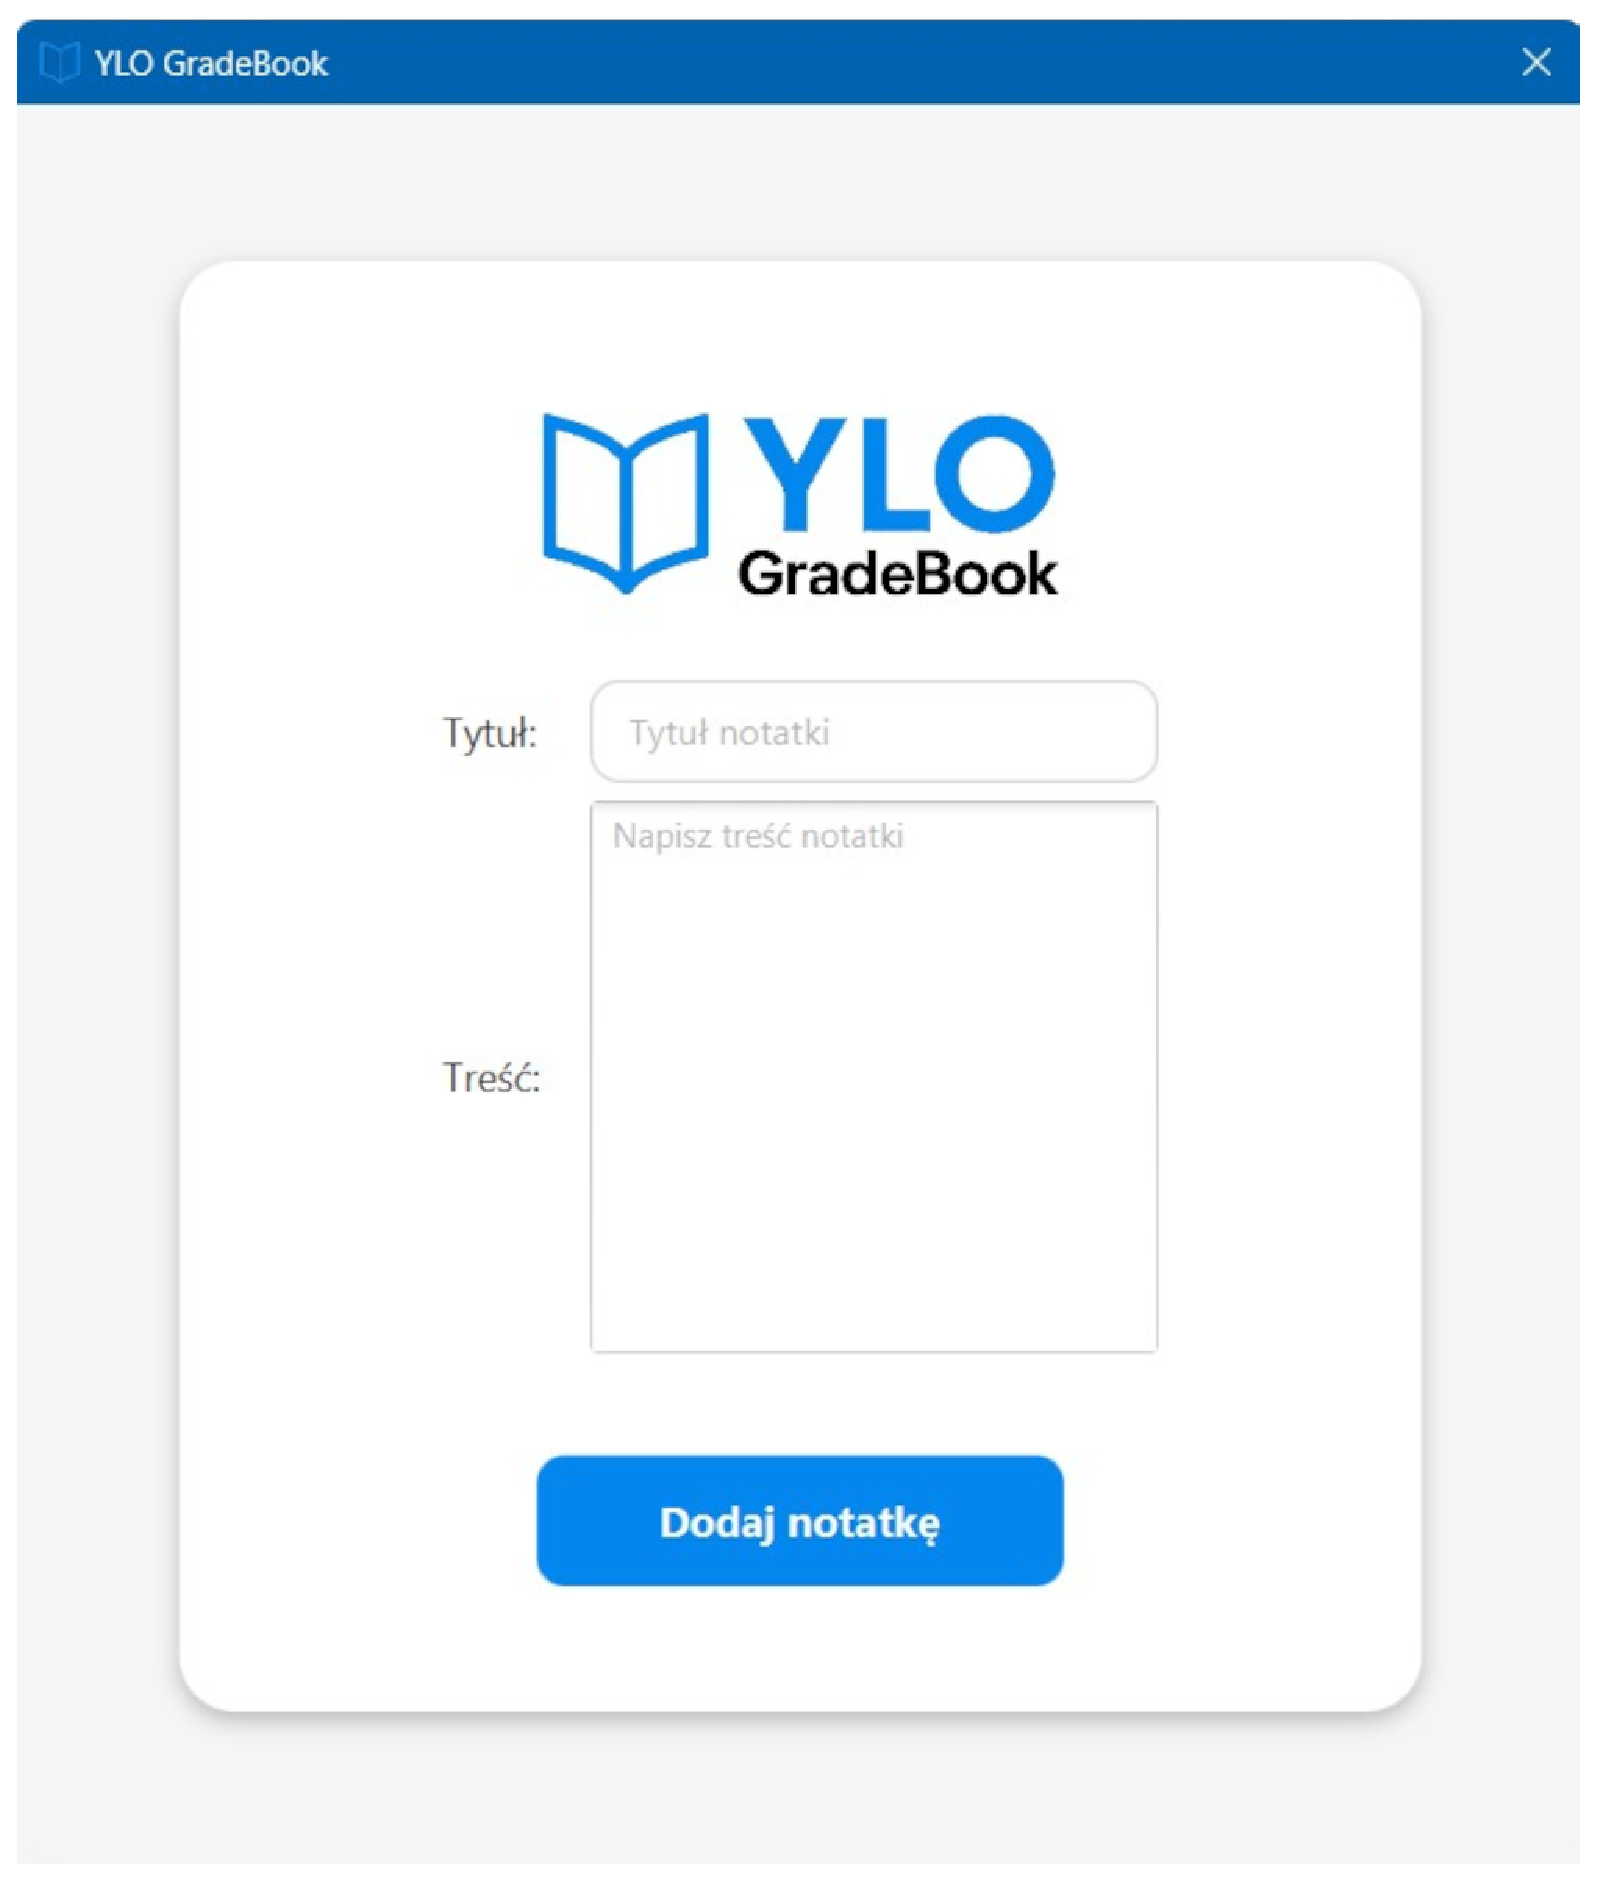
\includegraphics[width=0.9\textwidth]{figures/fig_0019.eps}
    \caption{PopUp — dodawanie notatki}
    \label{fig:popUpNote}
\end{figure}
\newpage
\section{Mechanizm alertów systemowych}

Aplikacja \texttt{YLO GradeBook} została wyposażona w system alertów, który informuje użytkownika o rezultacie wykonywanej operacji. Komunikaty pojawiają się m.in. przy:

\begin{itemize}
    \item nieprawidłowym logowaniu,
    \item błędnym wypełnieniu formularzy,
    \item anulowaniu operacji,
    \item wylogowaniu z sytemu,
\end{itemize}

Funkcjonalność ta została zrealizowana w klasie bazowej \texttt{SessionController}, która udostępnia wspólne metody. Dzięki ich zastosowaniu interfejs użytkownika informuje o przebiegu operacji w sposób przejrzysty, spójny i natychmiastowy.

Rozwiązanie to znacząco podnosi komfort i poczucie bezpieczeństwa przy wprowadzaniu danych do systemu.

Poniżej przedstawiono jeden z alertów pojawiających się podczas próby logowania.
\begin{figure}[H]
    \centering
    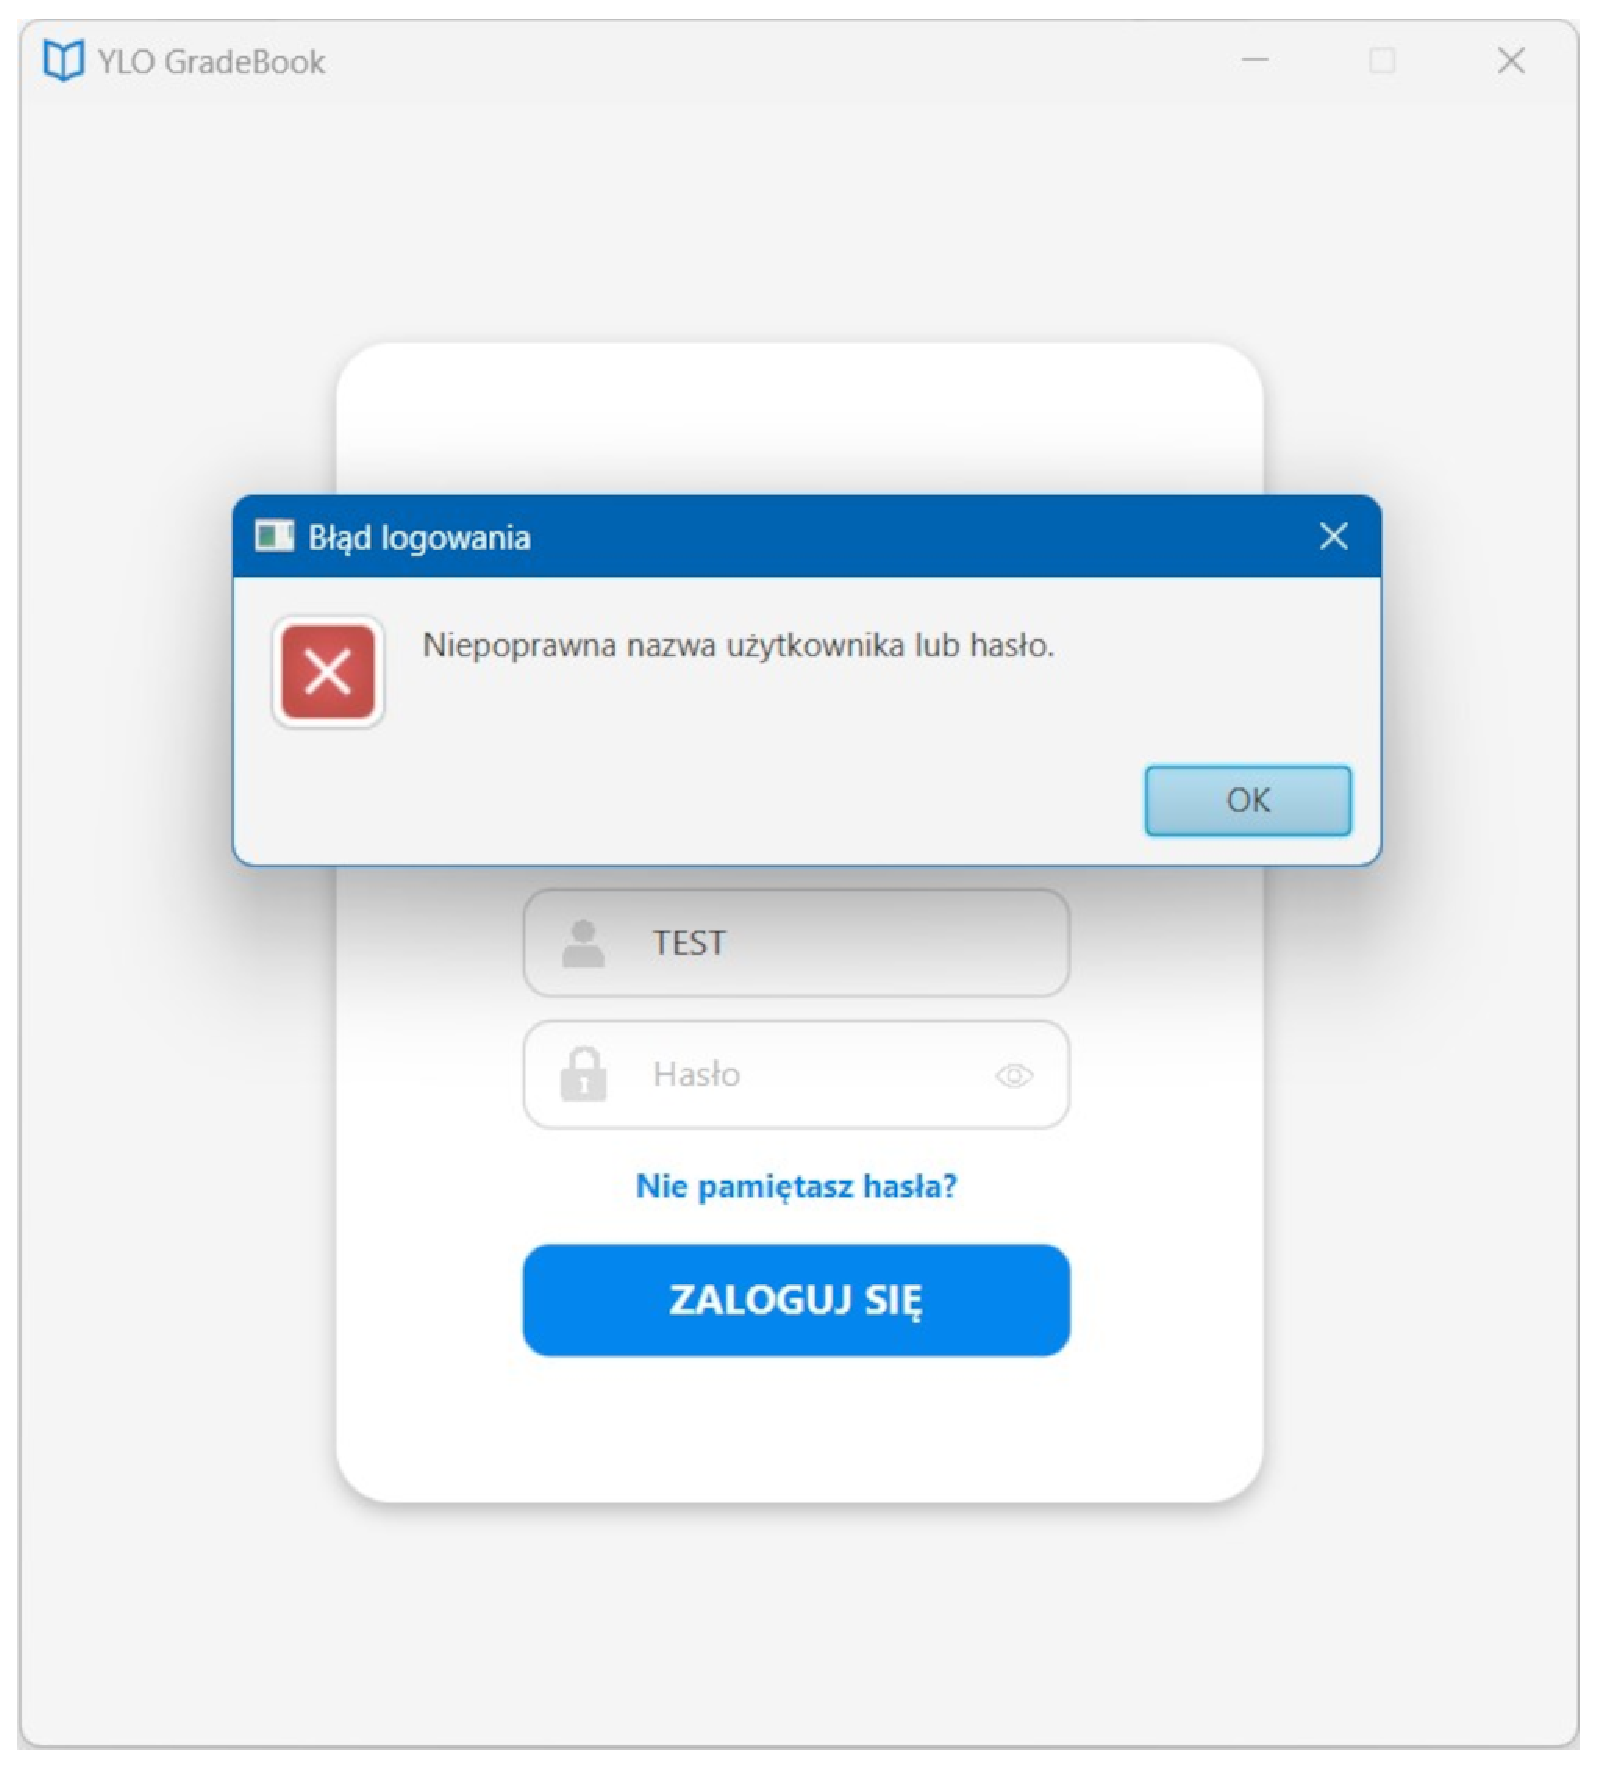
\includegraphics[width=0.9\textwidth]{figures/fig_0020.eps}
    \caption{Przykładowy alert systemowy — nieprawidłowe logowanie}
    \label{fig:alert}
\end{figure}


\chapter{Podsumowanie}
\label{cha:podsumowanie}

Celem projektu było stworzenie nowoczesnej, desktopowej aplikacji \texttt{YLO GradeBook}, która w przystępny sposób umożliwia zarządzanie ocenami uczniów pozwoli na organizaje pracy szkolnej placówki. Dzięki zastosowaniu języka \texttt{Java}, biblioteki \texttt{JavaFX} oraz relacyjnej bazy danych \texttt{MySQL}, udało się zaprojektować system wyróżniający się przejrzystością interfejsu, intuicyjnością obsługi oraz rozszerzalnością struktury danych.

Zrealizowane funkcjonalności umożliwiają:
\begin{itemize}
    \item logowanie użytkowników z rozróżnieniem ról (nauczyciel/uczeń),
    \item zarządzanie ocenami, terminami, notatkami i uwagami,
    \item dynamiczne wyświetlanie danych w zależności od kontekstu,
    \item edycję danych konta oraz resetowanie hasła,
    \item wyświetlanie średnich ocen,
    \item komfortową obsługę poprzez nowoczesny interfejs oparty o komponenty graficzne FXML oraz stylizację CSS.
\end{itemize}

Proces tworzenia aplikacji przebiegał etapowo: od analizy wymagań, przez projektowanie graficzne i implementację logiki, aż po testowanie oraz przygotowanie dokumentacji. 

Efekt końcowy spełnia założone cele, a dzięki przemyślanej strukturze kodu i bazy danych, możliwa jest dalsza rozbudowa aplikacji. Przykładowe opcje rozwoju:
\begin{itemize}
    \item dodanie weryfikacji dwuetapowej podczas logowania i resetowania hasła,
    \item zintegrowanie systemu z usługami poczty elektronicznej,
    \item rozszerzenie funkcjonalności o system obecności lub komunikator wewnętrzny,
\end{itemize}

Aplikacja \texttt{YLO GradeBook} stanowi stabilną i gotową do wdrożenia podstawę elektronicznego dziennika, ukierunkowaną na prostotę, czytelność i dopasowanie do realnych potrzeb użytkowników niezależnie od ich doświadczenia w pracy z komputerem.

\chapter{Instrukcja uruchomienia plikacji YLO GradeBook}
\label{cha:instrukcja}


\section{Wymagania środowiskowe}

Do poprawnego uruchomienia aplikacji \texttt{YLO GradeBook} wymagane jest przygotowanie środowiska zgodnie z poniższymi specyfikacjami programowymi:

\begin{itemize}
    \item \textbf{Środowisko JDK:} \texttt{OpenJDK 23.0.2} (Oracle)
    \item \textbf{JavaFX SDK:} wersja 23 (dołączona lokalnie do projektu)
    \item \textbf{IDE:} IntelliJ IDEA Community Edition 2024.3.3
    \item \textbf{Sterownik JDBC:} \texttt{mysql-connector-j-9.3.0}
    \item \textbf{Baza danych:} MariaDB 10.4.32 (środowisko \texttt{phpMyAdmin 5.2.1})
    \item \textbf{Panel sterowania:} \texttt{XAMPP Control Panel 3.3.0}
\end{itemize}

\textbf{Uwaga:} Domyślnym użytkownikiem serwera bazy danych jest \texttt{root}, a hasło pozostaje puste (\texttt{""}), zgodnie z domyślną konfiguracją XAMPP.

\subsubsection*{Zainstalowane wtyczki środowiska IntelliJ IDEA}

W trakcie pracy nad aplikacją wykorzystano kilka rozszerzeń środowiska IntelliJ IDEA. Poniżej zestawiono je z podziałem na wtyczki wymagane do poprawnego działania aplikacji oraz te, które służyły jedynie do wsparcia procesu implementacji lub dokumentacji.

\textbf{Wymagane do działania aplikacji:}
\begin{itemize}
    \item \textbf{JavaFX Runtime for Plugins} — wersja \texttt{1.0.4} \\
    (Źródło: JetBrains) \\
    Wtyczka niezbędna do uruchamiania komponentów \texttt{JavaFX}w środowisku IntelliJ.
\end{itemize}

\textbf{Wykorzystane pomocniczo (opcjonalne):}
\begin{itemize}
    \item \textbf{PlantUML Integration} — wersja \texttt{7.11.2-IJ2023.2} \\
    (Autorzy: Eugene Steinberg, Vojtech Krasa) \\
    Umożliwiła stworzenie diagramu klas systemu w postaci graficznej (rozdział 3).

    \item \textbf{PlantUML Parser} — wersja \texttt{0.0.9} \\
    (Autor: shuzijun) \\
    Parser współpracujący z powyższą wtyczką, pomocny przy generowaniu diagramu UML.

    \item \textbf{GitHub Copilot} — wersja \texttt{1.5.46-243} \\
    (Źródło: GitHub) \\
    Używana jako wsparcie przy pisaniu kodu, jednak nie jest wymagana do kompilacji ani działania aplikacji.
\end{itemize}


\section{Baza danych}

\begin{itemize}
    \item Do repozytorium dołączony jest plik \texttt{gradebook\_data\_base.sql}, który zawiera strukturę i przykładowe dane bazy danych.
    \item Po uruchomieniu serwera MySQL, należy zaimportować bazę danych do środowiska \texttt{phpMyAdmin}.
    \item Domyślny użytkownik: \texttt{root} \quad Hasło: *(puste lub zgodne z konfiguracją lokalną)*
    \item Po zaimportowaniu bazy danych należy upewnić się, że jej nazwa to \texttt{gradebook\_data\_base}, zgodnie z konfiguracją aplikacji w klasie DataBaseConnection.
\end{itemize}

\section{Kroki uruchomienia projektu YLO GradeBook}

Poniżej przedsatwiono listę kroków, prowadzącą do uruchomienia aplikacji.

\vspace{6pt}
\textbf{1. Klonowanie projektu z GitHub}

\begin{enumerate}
    \item Przejdź do repozytorium projektu: \\
    \texttt{https://github.com/oleiy/YLO-GradeBook}
    \item Pobierz repozytorium lokalnie, wykonując: \\
    \texttt{git clone https://github.com/oleiy/YLO-GradeBook}
    \item Otwórz folder projektu w środowisku \texttt{IntelliJ IDEA Community Edition 2024.3.3}
\end{enumerate}

\vspace{6pt}
\textbf{2. Konfiguracja środowiska Java i JavaFX}

\begin{enumerate}
    \item Skonfiguruj środowisko zgodnie z powyższą specyfikacją.
\end{enumerate}

\vspace{6pt}
\textbf{3. Dodanie sterownika JDBC}

\begin{enumerate}
    \item Umieść folder \texttt{mysql-connector-j-9.3.0} w katalogu projektu (dołączony do repozytorium)
    \item Dodaj go jako bibliotekę do projektu w \texttt{Project Structure → Modules}
\end{enumerate}

\vspace{6pt}
\textbf{4. Import bazy danych MySQL (phpMyAdmin)}

\begin{itemize}
    \item Uruchom środowisko \texttt{XAMPP Control Panel 3.3.0} i wystartuj moduł \texttt{MySQL}
    \item Otwórz \texttt{phpMyAdmin} w przeglądarce (\texttt{http://localhost/phpmyadmin})
    \item Utwórz nową bazę danych o nazwie \texttt{gradebook\_data\_base}
    \item Zaimportuj plik \texttt{gradebook\_data\_base.sql} z repozytorium
    \item Domyślny użytkownik: \texttt{root}, hasło: (puste)
\end{itemize}

\vspace{6pt}
\textbf{5. Uruchomienie aplikacji}

\begin{enumerate}
    \item Kliknij przycisk \texttt{Run} znajdując się w klasie Main.java
    \item Aplikacja otworzy ekran logowania
\end{enumerate}

\vspace{6pt}
\textbf{6. Dane testowe (do logowania)}

\begin{itemize}
    \item \textbf{Nauczyciel:} 
    \begin{itemize}
    \item nazwa użytkownika:\texttt{jan.nowak} 
    \item hasło: \texttt{jan}
    \end{itemize}
    \item \textbf{Uczeń:} 
    \begin{itemize}
    \item nazwa użytkownika:\texttt{igor.lis} 
    \item hasło: \texttt{igor}
    \end{itemize}
\end{itemize}


\vspace{6pt}
Po wykonaniu powyższych kroków środowisko programistyczne jest gotowe do pracy projektu YLO GradeBook. W przypadku trudności zaleca się weryfikację konfiguracji JavaFX oraz parametrów połączenia z bazą danych w klasie DataBaseConnection.
% Wyłączenie działania `ulem` na czas bibliografii
% Bibliografia
% Dodanie bibliografi do spisu treści
\addcontentsline{toc}{section}{\textbf{Bibliografia}}
\bibliographystyle{plain}
\bibliography{bibliografia}

% Przywrócenie działania `ulem`
\renewcommand{\emph}[1]{\uline{#1}}
\nocite{*}
\clearpage
% Dodanie spisu rysunków do spisu treści
\addcontentsline{toc}{section}{\textbf{Spis rysunków}}
\listoffigures
\clearpage

% \appendix
\chapter*{}
\label{cha:statement-A}
\makeatletter
\addcontentsline{toc}{section}{\textbf{Oświadczenie studenta o samodzielności pracy}}

\noindent
\begin{flushright}
    \begin{minipage}[!h]{10cm}
        Załącznik nr 2 do Zarządzenia nr 228/2021 Rektora Uniwersytetu Rzeszowskiego z dnia 1 grudnia 2021 roku w sprawie ustalenia procedury antyplagiatowej w Uniwersytecie Rzeszowskim
    \end{minipage}
\end{flushright}

\begin{center}
    \vspace*{10mm}
    \noindent  {\textbf{OŚWIADCZENIE STUDENTA O SAMODZIELNOŚCI PRACY} }
    \vspace*{10mm}
\end{center}

\noindent
\dotuline{\hspace{1.3cm}\@author\hspace{1.3cm}}\\ % Linia pozioma
{\small Imię (imiona) i nazwisko studenta }\\

\noindent \@faculty\\

\noindent \dotuline{\hspace{1.4cm}\@degreeprogramme \hspace{1.4cm}}\\
{\small Nazwa kierunku} \\

\noindent \dotuline{\hspace{1.8cm}\@noAlbum\hspace{1.9cm}}\\
{\small Numer albumu}

\begin{enumerate}
    \item Oświadczam, że moja praca projektowa pt.: \@titlePL
          \begin{enumerate}[label=\arabic*)]
              \item została przygotowana przeze mnie samodzielnie*,
              \item nie narusza praw autorskich w rozumieniu ustawy z dnia 4 lutego 1994 roku o prawie autorskim i prawach pokrewnych (t.j. Dz.U. z 2021 r., poz. 1062) oraz dóbr osobistych chronionych prawem cywilnym,
              \item nie zawiera danych i informacji, które uzyskałem/am w sposób niedozwolony,
              \item nie była podstawą otrzymania oceny z innego przedmiotu na uczelni wyższej ani mnie, ani innej osobie.
          \end{enumerate}
    \item Jednocześnie wyrażam zgodę/nie wyrażam zgody** na udostępnienie mojej pracy projektowej do celów naukowo--badawczych z poszanowaniem przepisów ustawy o prawie autorskim i prawach pokrewnych.
\end{enumerate}


\vspace*{10mm}

\noindent
\underline{\hspace{6cm}} \hfill \underline{\hspace{6cm}} \\ % Puste miejsce na miejscowość, data oraz podpis
\hspace*{13mm}(miejscowość, data)  \hspace*{63mm}(czytelny podpis studenta)
\vspace*{10mm}

\vfill
\noindent
* Uwzględniając merytoryczny wkład prowadzącego przedmiot \\
** -- niepotrzebne skreślić


\end{document}
